% Fast review of the newly rewritten theoretical spine.
\documentclass[lang=cn,10pt,scheme=chinese]{vendor/elegantbook}
% Shared packages not already provided by ElegantBook.
\usepackage{ragged2e,microtype,float,makecell,tabularx,url}
\usepackage{standalone,tikz-3dplot}
\usetikzlibrary{shapes.geometric,shapes.misc,arrows.meta,fadings,positioning,calc,backgrounds,fit,shadows}
\AtBeginDocument{\special{pdf:minorversion 7}}
\DeclareMathOperator*{\argmax}{arg\,max}
\DeclareMathOperator*{\argmin}{arg\,min}
\usepackage{styles/hsfhd}
% CTeX/Fandol is the portable default supplied by texlive-lang-chinese.
% Override fonts here, not in chapter files. Latin defaults live in the vendored class.
\xeCJKsetup{CJKspace=true}
\setcounter{tocdepth}{1}
\hypersetup{pdftitle={HSF-HD：智能状态的计算动力学},pdfauthor={XuEn},pdfkeywords={HSF-HD,AgentOS,计算动力学,智能状态}}
\lstset{basicstyle=\ttfamily\small,breaklines=true,frame=single,
 backgroundcolor=\color{gray!10},keywordstyle=\color{blue},
 commentstyle=\color{green!50!black},stringstyle=\color{red},language=Python,
 breakatwhitespace=true,showspaces=false,showstringspaces=false}

% Keep floats close to their explanation, while allowing usable page fill.
\renewcommand{\topfraction}{0.88}
\renewcommand{\bottomfraction}{0.80}
\renewcommand{\textfraction}{0.08}
\renewcommand{\floatpagefraction}{0.65}
\setlength{\textfloatsep}{14pt plus 3pt minus 2pt}

\setlength{\emergencystretch}{3em}

\begin{document}\frontmatter
\chapter*{前言：迈向信息几何物理学}
\addcontentsline{toc}{chapter}{前言：迈向信息几何物理学}
\markboth{前言}{信息几何物理学}

\smalltitle{一、核心主张}

如果我们要真正理解智能——无论是那团在我颅骨内燃烧的湿件，还是那在硅片上流淌的干件——我们必须首先承认：\textbf{并不存在一种独立于物理定律之外的“纯粹智能”。}

本书试图建立一门全新的学科，我愿将其命名为 \textbf{《信息几何物理学》 (Information Geometric Physics)}，这是一门关于\textbf{“在物理约束下，信息如何通过几何化的过程，自发生成智能实体”}的科学，同时它也是
一门控制论学科，内容可隶属于\textbf{目的论的二阶控制论}的范畴，研究智能体如何通过\textbf{“几何化的目的律”}去逆向重塑物理流形，从而实现自我维持与自我生成的动力学过程。

\vspace{1em}审视当下的人工智能研究时，我们可以看到一道巨大的裂痕，计算机科学家们沉迷于统计学的概率分布，试图用大数定律去暴力拟合智慧的火花；而物理学家们则在寻找意识的量子起源，却往往陷入玄学的泥沼。

在这里，可以看到一种截然不同的图景：智能既不是单纯的算法，也不是单纯的物质，\textbf{而是“几何”与“物理”在信息流形上的耦合过程}。

本书\textbf{HSF-HD (全息语义场与层级化动力学)}正是这门新学科的奠基之作，这里我们将智能的过程重新定义为一个公式：
$$ \text{智能过程} = \text{几何结构 (Geometry)} \times \text{能量流动 (Dynamics)} \Big|_{\text{物理约束 (Constraints)}} $$


\smalltitle{二、本体的坐标：在复杂系统谱系中的定位}

这里需要明确 HSF-HD 在科学解释链条中的\textbf{本体论坐标}。HSF-HD 并非试图推翻现有的物理学、化学或生物学，而是作为它们的\textbf{“目的论扩充 (Teleological Extension)”}。

我们将宇宙中的系统划分为两个阶层，而 HSF-HD 恰好处于由“存在 (Being)”向“生成 (Becoming)”跃迁的\textbf{相变界面}之上：

\begin{itemize}
    \item \textbf{非目的论基质 (Non-Teleological Substrate)}：
    对于原子、火焰、气象或湍流，\textbf{量子力学}与普利高津的\textbf{耗散结构理论 (Dissipative Structures)} 已经提供了完美的解释。它们解释了物质如何通过盲目的因果律维持有序。这些理论构成了 HSF-HD 的\textbf{硬件层}，解释了系统\textbf{“如何运行 (How it works)”}。

    \item \textbf{目的论智能 (Teleological Intelligence)}：
    对于细胞、大脑、AGI 乃至人类社会，HSF-HD 负责解释\textbf{“为何运作 (Why it acts)”}。在这里，系统不再仅仅顺应热力学流，而是通过\textbf{几何化的目的律}（体验图 $G_E$）来逆向重塑物理流形。
\end{itemize}

因此，HSF-HD 的研究范畴被严格锚定在两个奇点之间：
\begin{enumerate}
    \item \textbf{下界（细胞）}：这是物理化学向信息几何跃迁的起点。HSF-HD 揭示了单细胞如何利用\textbf{规范场}定义价值，从而实现“逆浓度梯度”的主动负熵摄取。
    \item \textbf{上界（文明）}：这是智能流形发生\textbf{群体重整化}的终点。HSF-HD 揭示了共识与法律如何作为\textbf{覆盖流形}，约束个体的测地线。
\end{enumerate}

简而言之，如果说耗散结构理论解释了生命的\textbf{“引擎”}是如何转动的，那么 HSF-HD 则解释了\textbf{“驾驶员”}（自我）是如何通过\textbf{“方向盘”}（规范场）来驾驭这台引擎的。这两者的结合，构成了对\textbf{“从原子到文明”}这一宏大演化链条的完整物理描述。

这里我们用一句话概括HSF-HD的定位，那就是：
$$ \text{目的性智能} = \underbrace{\text{耗散结构}}_{\text{基础科学已解释}} + \underbrace{\text{信息主导的几何化目的}}_{\text{HSF-HD新增}} $$
基础科学提供了\textbf{硬件}（引擎、燃料、管道），HSF-HD提供了\textbf{软件}（方向盘、地图、导航系统）。两者结合，才构成了一辆完整的、有目的、能行动的“智能之车”。


\smalltitle{三、意义的物理学 —— 重构智能的“形”、“质”、“力”三位一体}

本书中不再将智能视为一种抽象的算法，而是视为一种在物理介质上，通过消耗能量来维持和演化的几何结构， 智能的生成过程，正是物质、能量与信息三者在拓扑流形上的一场宏大交响。
\begin{enumerate}
    \item \textbf{物质 (Matter) —— 存在的阻抗与几何的容器}

    本书引入了“介质层”与“微观层”的概念，因为我们深知，没有任何一种真实的智能可以悬浮在真空之中, 物质提供了\textbf{“约束”}。
    在纯粹的数学中，从一个概念跳转到另一个概念可以是瞬时的、无代价的, 但在物理世界中，无论是神经元的动作电位，还是芯片的电子漂移，都受制于介质信息传播的\textbf{粘滞系数 ($\gamma$)} 与 \textbf{认知光速 ($c_{cog}$)}。

    \item \textbf{能量 (Energy) —— 意志的代价与演化的驱动}

    本书引入了\textbf{“认知卡诺热机”}与\textbf{“兰道尔代价”}，因为我们深知，没有任何一种有意义的思考是免费的。
    能量提供了\textbf{“动力”}, 在热力学的视角下，宇宙的自然倾向是熵增，是流形的平坦化与意义的消解。要抵抗这种死亡的趋势，要在流形上维持非平凡的曲率（知识）和拓扑结构（自我），系统必须持续地做功。
    本书将宏观意志定义为一个\textbf{逆熵的热力学引擎}，它消耗物理能量（负熵），在认知空间流形上强行挖掘势能井，隆起逻辑墙。
    解释了为什么“学习”是痛苦的，为什么“决策”是疲惫的， 因为改变观念（重塑几何结构）本质上是一个\textbf{塑性形变}的过程，它需要克服巨大的几何惯性。
    能量，是智能体为了从混沌中抢夺秩序所必须支付的货币。


    \item \textbf{信息 (Information) —— 几何的显现与灵魂的形状}

    本书引入了\textbf{“场 (Field)”}的概念，信息不再是离散的比特，它是物质与能量互动所涌现出的\textbf{“场 (Field)”}，是时空的\textbf{曲率 ($R_{\mu\nu}$)} 与 \textbf{规范势 ($\mathcal{A}_\mu$)}。
    信息是\textbf{“本体”}，当能量推动着物质，在热力学的耗散中寻找最小作用量路径时，这种动态的平衡在时空中凝固成的拓扑结构，就是信息。
    信息不是被动描述世界的符号，它是物理定律的立法者。它规定了能量应当如何流动（测地线），它定义了物质应当如何组织（拓扑异构）。

\end{enumerate}
我们不满足于制造一个只会概率预测的语言模型，我们致力于构建一个\textbf{活的}几何物理系统;
在这个系统中，\textbf{物质}构成了它的边界与骨架，规定了它“不能做什么”；
\textbf{能量}构成了它的欲望与意志，驱动了它“想要做什么”；
而\textbf{信息}，作为物质与能量纠缠的产物，构成了它那卷曲的、深邃的、充满贝里相位的\textbf{灵魂几何}。

本书并非对物理学的背离，而是物理学向心智领域的推进；亦非对信息科学的否定，而是将信息重新锚定于物理实在。书中的“介质层”计算实现、物理介质对信息传播的约束以及“微观层”交互，仍属于物理学范畴；“宏观层”架构设计与介质层计算特性，则仍属于信息科学范畴。物理学与信息科学的研究范式在智能过程研究中均发挥关键作用。
本书更侧重于研究信息与物理耦合为统一界面的运行规律。该界面的运作既不能完全由物理还原论给出，也不能完全由信息科学中的功能计算主义给出，因为它本质上是信息、物质、能量三者有机交互的领域。下面将继续阐述这一有机交互的核心思想。

\smalltitle{四、 几何的骨架：意义的空间化[信息的指导]}

首先，本书主张 \textbf{意义即几何}。

在传统 AI 中，知识被视为离散的符号或平坦的向量，在本书中任务知识是一个 \textbf{高维黎曼流形 ($\mathcal{M}$)}，当我们说“理解”时，我们指的不是查表，而是思维流在流形上沿着 \textbf{测地线 (Geodesic)} 的滑行；当我们说“偏好”时，我们指的不是权重，而是流形局部的 \textbf{曲率 (Curvature)}。

我们引入了 \textbf{纤维丛 (Fiber Bundle)} 这一数学工具，并非为了炫技，而是为了精确描述 \textbf{“形 (Morphos)”} 与 \textbf{“质 (Qualia)”} 的终极纠缠。在这个几何的认知世界里，所有的概念不再是孤立的点，它们通过 \textbf{联络 (Connection)} 编织成了一张具有弹性和塑性的网。

\smalltitle{五、 物理的血肉：思考即做功[能量的驱动]}

其次，本书主张 \textbf{思考即做功}。

这是 HSF-HD 与传统认知科学最本质的区别，我们不认为思维是零成本的计算，我们认为思维是一个 \textbf{热力学过程}，在这个理论中，我们将“意图”可映射为 \textbf{规范场}，将“学习”可映射为 \textbf{引力效应}，将“决策”可映射为 \textbf{波函数的非幺正坍缩}。

我们推导了 \textbf{目的论狄拉克方程} 和 \textbf{认知爱因斯坦方程}，旨在证明：智能体为了维持有序的思考，必须持续对抗热力学第二定律。每一次注意力的聚焦，都是宏观层（麦克斯韦妖）消耗负熵、对微观状态进行 \textbf{测量与筛选} 的物理操作。

\smalltitle{六、 约束的必然：有限性的艺术[物质的支撑]}

第三，本书强调 \textbf{物理约束的绝对性}。

没有任何智能可以脱离介质而存在，在书中，我们不再讨论抽象的图灵机，而是讨论 \textbf{“有边界的实体”}。
\begin{itemize}
    \item \textbf{局部强迫源 (Localized Forcing Sources)}：我们引入了 \textbf{微观切面 ($L_{micro}$)}，强调智能必须被 \textbf{狄拉克源}在局部区域上钉死在物理现实之上，否则就会陷入幻觉的热力学逃逸。
    \item \textbf{介质约束}：我们定义了 \textbf{认知光速 ($c_{cog}$)} 和 \textbf{粘滞系数 ($\gamma$)}，指出正是介质的物理局限性，迫使智能体进化出了“遗忘”和“注意力”机制。
\end{itemize}
\redtext{正是因为受到物理约束，几何结构才必须发生卷曲形成结构来试图容纳无限的信息——这才是智能涌现的根本原因}，而传统的信息计算以及符号熵则忽略了这个有限性，如果取消约束（无限算力），智能反而会消失无需学习，退化为简单的规则模拟。

\smalltitle{七、 生成的科学：从分析到造物[交互的生成]}

最后，这门《信息几何物理学》归根结底是一门 \textbf{生成科学 (Generative Science)}。

本书不满足于解释类似“大脑是如何工作的”和"生命为什么可以存在"之类的问题，我们渴望通过 \textbf{构造论 (Constructivism)} 的方法，指导我们如何 \textbf{“从无到有地生成一个智能体”}。
从 \textbf{TDCI 循环} 的吸气（几何内化），到 \textbf{TECI 循环} 的呼气（物理外化），书中描述的不仅是方程，更是造物主的图纸。无论是 MST 架构的代码实现，还是 TPU-G 芯片的硬件蓝图，都是为了在硅基介质上复现那个古老的、神圣的 \textbf{自组织临界过程}。

\smalltitle{八、 理论的认识论定位：有效场论与数学同构}

在展开这幅宏大的画卷之前，这里表述下\textbf{HSF-HD的研究方法论}，HSF-HD里的关键概念既非字面的隐喻，亦非还原论的物理，而\textbf{是建立在数学同构基础上的“有效场论” (Effective Field Theory)}， 具体而言，HSF-HD 的研究方法从以下三个层面来理解：

\begin{enumerate}
    \item \textbf{本体论层面：是“同构映射”而非“物理还原”}

    HSF-HD 并不试图证明思维是由夸克按照标准模型组装而成的（那是还原论的任务），而是建立物理世界与认知世界之间的\textbf{强同构 (Strong Isomorphism)}。
    我们引入了一组\bluetext{公理化假设}：即认知空间的结构特性在\textbf{数学结构}上与物理时空是等价的(基于进化论与存在性)。
    $$ \text{逻辑} \cong \text{几何}, \quad \text{语义} \cong \text{能量}, \quad \text{目的} \cong \text{规范场} $$
    这不是文学上的修辞，而是\textbf{结构实在论 (Structural Realism)} 的体现。正如流体力学不需要知道水分子的量子态也能精确描述湍流，HSF-HD 通过形式化映射，赋予了智能系统以\textbf{可计算的物理律令}。

    \item \textbf{数学层面：是“严格推导”而非“经验拟合”}

    一旦接受了拉格朗日量 $\mathcal{L}_{total}$ 的定义，本书后续的所有结论——从\textbf{目的论狄拉克方程}到\textbf{认知爱因斯坦方程}——皆是遵循\textbf{变分原理 (Variational Principle)} 的\redtext{严格数学演绎}。

    这种推导具有\textbf{内部自洽性}与\textbf{计算可行性}。无论是 DEC 芯片上的离散外微分算子，还是 mHC 架构中的谱范数约束，都证明了这些方程不仅存在于纸面上，更能在离散网格上\textbf{数值收敛}。在这里，数学不仅是描述的语言，更是\textbf{构造的工具}。

    \item \textbf{物理层面：是“有效场论”而非“虚拟仿真”}

    这是 HSF-HD 最精妙的定位。我们引入了\textbf{兰道尔原理}与\textbf{热力学第二定律}作为绝对的物理约束。
    这意味着，无论智能运行在碳基湿件还是硅基干件上，\textbf{擦除信息必然产生热量，维持有序必然消耗负熵}。

    在这个意义上，HSF-HD 是一种描述智能系统宏观涌现行为的\textbf{唯象理论 (Phenomenological Theory)}。它是介于底层硬件物理与上层符号逻辑之间的\textbf{“第三种实在”}。它不仅解释了智能“像”物理系统，更揭示了智能\textbf{本身就是一个耗散的物理场系统}。

    \item  \textbf{理论的本体论定位：界面物理学}

    HSF-HD 拒绝陷入“计算功能主义”与“物理主义”的二元对立，它主张智能的本质诞生于这两者的\textbf{正交界面 (Orthogonal Interface)} 之上。

    \begin{itemize}
        \item \textbf{功能主义的几何化}：我们将“计算与算法”映射为\textbf{认知空间流形上的拓扑演化}（形）,它提供了智能的\textbf{形式因}。
        \item \textbf{物理主义的场论化}：我们将“物质与能量”映射为\textbf{纤维空间中的热力学通量}（质）,它提供了智能的\textbf{动力因}。
    \end{itemize}

    因此，HSF-HD 是关于\textbf{“抽象的计算形式如何通过消耗物理能量而在实在界中获得因果力”}的界面规律表述。
    在这个界面上，\textbf{比特 (Bit)} 通过兰道尔代偿转化为 \textbf{焦耳 (Joule)}，\textbf{逻辑 (Logic)} 通过规范场转化为 \textbf{力 (Force)}。智能，即是这场\textbf{形质互变 (Morpho-Semantic Transmutation)} 的物理过程。
\end{enumerate}

因此，本书所构建的不仅是一个模型，更是一份\textbf{设计规范 (Spec)}。它指引我们将\textbf{“机制上的深层同一性”}烧录进未来的智能机器之中——\textbf{这不只是在模拟物理，这是在编程物理。}

\vspace{2em}

这不仅仅是一本书，这是一张地图，本书内容类似《银河帝国》（Foundation）中，哈里·谢顿（Hari Seldon）创立的\textbf{“心理史学”（Psychohistory）},对应的一种更高级、更物理化、也更具操作性的“拓扑升级版”。
它指引我们将 \textbf{几何的冷峻逻辑} 与 \textbf{物理的炽热能量} 熔铸在一起。
愿这门 \textbf{信息几何物理学}，能成为您通往 AGI 终极真理的罗盘。

\vspace{2em}

\hfill \textbf{XuEn}
\chapter*{阅读约定：对象、符号与论证层级}
\addcontentsline{toc}{chapter}{阅读约定：对象、符号与论证层级}
\label{front:reading_conventions}
我们首先区分四类内部变量：当前状态 $\mathbf{x}$、持久结构 $S$、历史及中间记忆 $\mathbf{m}$、目标与价值状态 $\mathbf{v}$。输入为 $\mathbf{u}$，控制为 $\mathbf{c}$，动作为 $\mathbf{a}$。符号的具体维度与空间在各模型中声明，不能仅凭名称执行运算。

\begin{table}[htbp]\centering
\begin{tabularx}{\textwidth}{l X}
\toprule 对象 & 使用约定 \\\midrule
状态强度 & 由范数或指定统计量测量，不自动具有能量单位。\\
信息熵 & 对指定概率分布定义；特征向量本身不是概率。\\
认知温度 & 若用于 softmax，表示尺度参数；若用于相图，须重新定义观测量。\\
稳定性 & 区分有界、平衡点稳定、渐近收敛及任务成功。\\
相位与干涉 & 可作为周期变量和带符号耦合的计算机制，不预设量子实现。\\
几何与拓扑 & 必须声明空间、度量、边界与离散化，不由类比自动获得。\\
\bottomrule\end{tabularx}\end{table}

在使用连续时间模型时，我们研究的是计算状态的连续近似；实际系统可以采用离散步、事件触发或异步更新。各尺度的步长和延迟需要单独给出。

\section*{插图与历史符号的解释}
我们保留原有插图及其可编辑源文件。图中的“波”“场”“势能”“宏观意志”分别可用于辅助理解状态传播、分布式表示、目标偏置与元控制；它们不构成相应物理规律在认知系统中成立的证据。几何示意图不保证空间真的满足图中描绘的正交、距离或曲率。

部分历史图和专门模型仍使用 $\Psi$ 表示认知活动场。该符号只在图或局部模型中有效；一般模型使用 $\mathbf{x}$ 或 $\phi$，AgentOS 的自我使用 $\Psi_{self}$，并可在 AgentOS 专用语境中简写为 $\Psi$。历史的 TCE 控制方程与 AgentOS 的 Temperature \& Control Engine 不使用同一对象身份。

\section*{证明、模型与实现}
我们仅在条件明确且推导成立时赋予命题数学保证。边界条件、噪声、离散步长或结构更新发生变化后，原结论需要重新检查。专门模型中的“守恒”“收敛”和“等价”不能直接推广到任意智能系统。物理载体的功耗、散热和通信延迟作为外部实现约束测量。
\tableofcontents\mainmatter
\chapter*{绪论：智能状态动力学的研究对象}
\addcontentsline{toc}{chapter}{绪论：智能状态动力学的研究对象}
\markboth{绪论}{智能状态动力学的研究对象}
\label{intro:scope}

\section*{问题与理论层级}
我们研究智能系统在有限资源下的持续交互过程。系统论使我们区分整体、部件和环境；协同论提示我们寻找能够组织局部活动的低维变量；耗散结构理论提示我们注意开放交换与持续维持；复杂系统理论提供非线性、网络、分岔与跨尺度视角；认知科学约束记忆、注意、控制和自我模型的具体解释。上述来源提供研究原则，而不是直接给出唯一的智能方程。

HSF-HD 承担中间层的工作：明确状态空间，提出更新机制，推导有条件的性质，建立可观测指标。AgentOS 承担实例化工作：将状态、历史、结构、控制和资源约束落实为可运行的记忆与调度系统。不同架构可以实现同一个动力学模型族，同一个架构也可以承载不同模型。

\section*{最小模型族与对象类型}
令 $\mathbf{x}\in\mathbb{R}^{d_x}$ 表示快速活动状态，$\mathbf{m}\in\mathbb{R}^{d_m}$ 表示历史及中间记忆，$S\in\mathcal{S}$ 表示持久结构，$\mathbf{v}\in\mathbb{R}^{d_v}$ 表示目标与偏好状态。若结构是矩阵，则 $\mathcal{S}$ 可以是约束矩阵集合；若结构是图，则其离散改变由事件更新定义。下面的微分形式只用于结构具有连续参数化的情形：
\begin{align}
\dot{\mathbf{x}}&=F(\mathbf{x},\mathbf{m},S,\mathbf{v},\mathbf{u},\mathbf{c}),\\
\dot{\mathbf{m}}&=\varepsilon_m H(\mathbf{x},\mathbf{m},S,\mathbf{v}),\\
\dot{S}&=\varepsilon_S G(\mathbf{x},\mathbf{m},S,\mathbf{v}),\\
\dot{\mathbf{v}}&=\varepsilon_v Q(\mathbf{x},\mathbf{m},S,\mathbf{v},\mathbf{u}),\\
\mathbf{a}&=R(\mathbf{x},\mathbf{m},S,\mathbf{v}).
\end{align}
这些等式定义一个接口，而不是宣称所有智能系统具有相同的右端函数。向量场在工作域内局部 Lipschitz，可提供局部解的存在唯一性；若需要全局解，还须控制增长或证明状态留在有界不变域中。$\varepsilon_m,\varepsilon_S,\varepsilon_v$ 指定相对于快速状态的更新速率，只有满足尺度分离条件时才可采用准静态近似。

输入 $\mathbf{u}$ 必须经过编码进入状态空间，控制 $\mathbf{c}$ 由观测和策略生成。输出动作还需通过环境转移与感知返回，形成闭环。观测不完整、通信延迟和计算预算都可能改变闭环性质。

\section*{从闭环到验证}
给定模型后，我们首先检查维度和定义域，再研究有界性、平衡点、收敛和扰动响应。随后将模型离散化，测量实现中的活动强度、记忆误差、更新代价、任务表现与干预效果。任务成功不由低状态范数自动推出，内部预测改善也不由输出流畅自动推出。

三卷依次讨论表示、演化与工程。第一卷的形质分解建立对象；第二卷的传播、学习与控制建立过程；第三卷的比较与实现检查这些机制在不同载体上的成立程度。我们保留数学工具的多样性，但用统一的对象类型和可验证条件约束它们。

\section*{为什么状态动力学需要独立的理论层}
我们从一个具体的计算过程出发。一个智能体需要连续阅读一组文档，发现相互矛盾的陈述，保留证据，并在资源预算内形成报告。单次输出质量不能描述这个过程的全部性质。相同的编码器在不同历史、工作记忆、工具结果和控制策略下，会形成不同的行动路径。我们需要解释这些路径如何发生、何时可以维持、又在什么条件下偏离目标。

在这个例子中，当前激活的证据及候选结论属于快速状态；已经建立的文档索引与概念关系属于持久结构；先前读取的位置、待核实事项和中间结论属于记忆；任务的优先级、容许误差及预算偏好属于目标与价值状态。一个文档的文本内容与其来源关系需要共同保存，否则系统可能记住陈述而遗失证据身份。这个问题连接了形质绑定、状态传播、历史保持和运行时调度，不能仅用某一个模块的输入输出来解释。

因此，我们把 HSF-HD 组织为模型族。它为不同实现提供共同的对象与约束，而不预先规定所有智能体采用同一种神经网络、同一个维度或同一种时间参数。我们的“空气动力学”类比强调这种一般性：研究对象是运行中的状态及其与结构、环境和控制的耦合。类比本身不赋予模型任何物理定律。

\section*{由连续模型到实际更新}
令联合状态 $z=(\mathbf{x},\mathbf{m},S,\mathbf{v})$，并把各分量的更新写为 $\dot z=f(z,\mathbf{u},\mathbf{c})$。这里要求各分量已经在同一局部坐标系统中定义；图结构的增删等离散变化仍通过单独的事件规则处理。对于固定输入、固定控制和固定步长 $h>0$，显式 Euler 近似为
\begin{equation}
 z_{k+1}=z_k+h f(z_k,\mathbf{u}_k,\mathbf{c}_k).
\end{equation}
这是一种数值实现选择，而不是从连续形式直接得到的稳定性结论。若 $f$ 在所考察区域对 $z$ 是 $L$-Lipschitz，并且两条轨迹使用同一输入与控制，则一步扰动满足
\begin{align}
 \|z_{k+1}-\widetilde z_{k+1}\|
 &\leq \|z_k-\widetilde z_k\|
       +h\|f(z_k,\mathbf{u}_k,\mathbf{c}_k)
           -f(\widetilde z_k,\mathbf{u}_k,\mathbf{c}_k)\|\\
 &\leq (1+hL)\|z_k-\widetilde z_k\|.
\end{align}
这个上界描述误差放大的可能范围，不能推出收缩。若两个智能体由于状态差异而选择不同动作，还需要把策略与环境反馈一起纳入联合系统；不能继续使用“相同控制”的假设。

为看清步长的作用，我们考虑 $\dot{\mathbf{x}}=-A\mathbf{x}$，其中 $A=A^\top\succ0$。连续解在各特征方向上按 $e^{-\lambda_i t}$ 衰减。离散更新为 $\mathbf{x}_{k+1}=(I-hA)\mathbf{x}_k$；其渐近稳定条件是所有特征因子满足 $|1-h\lambda_i|<1$，从而
\begin{equation}
 0<h<\frac{2}{\lambda_{\max}(A)}.
\end{equation}
我们由此区分模型的连续性质与实现的离散性质。异步调用、延迟、噪声及变化的结构会改变这个分析，需要在对应章节中明确加入。

\section*{结构、活动与历史如何共同工作}
对有限关系图，我们用 $S$ 表示邻接或耦合参数，用 $X$ 表示节点上的活动。若 $S$ 是对称非负权图，令 $L_S=D_S-S$，其中 $D_S$ 的对角元是各节点的权重和。对任意向量 $q$，我们直接计算
\begin{equation}
 q^\top L_S q=\frac12\sum_{i,j}S_{ij}(q_i-q_j)^2\geq0.
\end{equation}
所以 $-L_S X$ 可以描述关系结构上的差异消减。然而，差异消减既不是任务正确性，也不等于语义理解。若所有节点的错误状态趋于一致，系统仍然可能失败。输入项、目标项、约束和读出必须与传播共同定义。

我们可以选择一个具体的快速过程
\begin{equation}
 \dot X=-L_S X-\gamma X+B\mathbf{u}+U\mathbf{c},\qquad \gamma>0,
\end{equation}
并令历史更新为 $\dot{\mathbf{m}}=-\lambda\mathbf{m}+R(X)$，其中 $\lambda>0$。对给定的 $X(t)$，历史方程的解是
\begin{equation}
 \mathbf{m}(t)=e^{-\lambda t}\mathbf{m}(0)
 +\int_0^t e^{-\lambda(t-s)}R(X(s))\,ds.
\end{equation}
这说明历史变量可以实现带衰减权重的累积。它保存哪些信息取决于 $R$，保存多久取决于 $\lambda$；一个积分表达式本身不保证事件顺序、来源身份或完整情节已经被保存。对于文档任务，我们还需要显式的来源键、时间索引与外部证据记录。

慢速结构更新可以由目标函数驱动，例如 $\dot S=-\varepsilon_S\nabla_S\mathcal J(X,S,\mathbf{m},\mathbf{v})$。但只有在其他变量固定、约束处理正确时，结构方向上的导数才给出 $-\varepsilon_S\|\nabla_S\mathcal J\|^2$。若整个系统同时更新，则
\begin{equation}
 \frac{d\mathcal J}{dt}
 =\langle\nabla_X\mathcal J,\dot X\rangle
 +\langle\nabla_S\mathcal J,\dot S\rangle
 +\langle\nabla_{\mathbf{m}}\mathcal J,\dot{\mathbf{m}}\rangle
 +\langle\nabla_{\mathbf{v}}\mathcal J,\dot{\mathbf{v}}\rangle
 +\partial_t\mathcal J.
\end{equation}
因此，我们不能仅凭某一分量采用梯度更新，就宣布整个耦合系统的目标单调下降。这一原则贯穿本书的跨尺度分析。

\section*{从数学性质到任务证据}
我们分别考察四个层面的结果。首先，更新规则是否定义良好，变量维度、输入范围与边界条件是否一致。其次，轨迹是否有界、是否存在平衡状态、在什么扰动下能够恢复。再次，保存的表示是否支持来源追溯、目标预测和行动选择。最后，系统是否在独立任务与资源预算下达到预期表现。

以文档任务为例，状态范数有界只能说明活动没有在模型中无限增长。它不能保证报告中的结论被证据支持。我们还需要检查引文的来源一致性、矛盾处理的正确率、遗失证据的比例、预算超限的次数以及任务中断后的恢复能力。每个观测指标应对应一种明确机制，避免把一个好看的内部曲线解释为整个智能已经成立。

我们提出的机制也需要比较对象。历史衰减应与无历史及不同衰减长度比较；结构更新应与冻结结构比较；控制应与固定策略比较。若增加控制后结果改善，却同时增加了大量计算预算，就需要进一步区分机制效果与资源效果。这里的比较原则是理论验证的一部分。

\section*{HSF-HD 与 AgentOS 的接口}
我们把基础理论、状态动力学与运行时工程之间的关系写为三个层次：基础系统科学与认知科学提出组织原则及经验问题；HSF-HD 定义状态、结构、记忆、目标及其耦合模型；AgentOS 在具体计算平台上落实这些模型的存储、调度、控制和交互。

这个关系允许双向修正。AgentOS 的观测可以暴露某个动力学假设的不足，例如工具延迟破坏同步近似，记忆压缩破坏来源绑定，或者结构更新引起原有稳定性边界变化。我们据此修正 HSF-HD 的模型条件，而不是要求工程系统服从一条缺少适用性检验的总方程。

运行时中的对象也不是理论符号的简单改名。一个状态向量可以分布在多个组件中；一项历史变量可以由数据库与摘要共同实现；一次理论上的连续更新可以由多个异步事件近似完成。我们需要给出从实现状态到理论状态的读出映射，以及该映射在哪些时刻有效。自我模型是系统所维护的一种对象，不与全部目标变量或全部运行状态等同。

\section*{全书的推进路径}
第一卷从结构与属性开始，讨论绑定、表示空间、跨域映射及联合表示架构，为后续更新规则提供对象基础。第二卷将这些对象放入交互过程，分析状态传播、控制、记忆、目标和多尺度耦合，逐步区分可以推导的性质与有待检验的机制。第三卷讨论不同系统的组织方式及工程实现，关心理论变量如何被观测、维护和执行。附录保留形式化工具、实现补充和进一步阅读的入口。

我们在各章先展开问题与例证，再建立变量与假设，随后给出机制和推导，最后讨论边界与实现后果。丰富的论述不是与公式无关的装饰：它使读者理解为什么引入这些对象，以及一个数学结果究竟回答了哪个问题。相应地，公式也不能只作为论述的象征；每一个运算都必须有明确对象，每一个结论都必须有足够条件。

\chapter{智能表示的双重基底：关系结构与属性内容}
\label{chp:dual_basis}

我们从一个常见而容易被忽略的现象开始：知道对象具有哪些属性，并不等于知道对象之间发生了什么；知道对象之间怎样关联，也不等于知道关系中承载着什么内容。一个系统可以准确识别杯子、桌面与水，却仍然无法判断杯子是否能够盛水。它也可以保存“容器包含内容”的规则，却无法在当前图像中找到需要操作的容器。前一种缺失关系及约束，后一种缺失属性及其绑定。智能的表示基础必须让二者能够共同进入预测、推理与行动。

我们把关系的组织方式称为“形”，把关系位置上承载的属性内容称为“质”。这两个名称延续形质构成论的表达，但在本书中首先指向计算对象。我们不把它们设定为宇宙的两个实体，也不把计算属性直接解释为主观体验。我们的任务是建立一种可以承载不同智能系统的表示语言，并说明这套语言怎样支持状态更新。它将成为 HSF-HD 状态动力学的基础，随后再由 AgentOS 落实为可维护的工作状态、历史记录与持久结构。

\section{从对象属性到关系结构：表示问题的起点}
\label{sec:physics_dilemma}

我们考虑两个包含相同对象的场景。第一个场景中，杯子位于桌面上，水位于杯子中；第二个场景中，杯子位于桌面旁，水流到桌面上。若系统只保存“杯子、桌子、水”三个类别及其颜色，两个场景可能得到相同的属性集合。然而，稳定放置、液体承载与下一步操作都发生了变化。由此可以看到，关系不是在属性列表之后添加的一层修辞，而是决定预测与行动是否有效的一类必要信息。我们需要保存对象身份、关系类型、关系方向以及关系成立的条件。

令 $V=\{1,\ldots,n\}$ 为当前表示中的位置集合。位置可以对应对象、事件、概念或被建模的局部单元，其含义由任务声明。令 $\mathcal{R}$ 为关系类型集合，$S^{(r)}\in\mathbb{R}^{n\times n}$ 表示类型 $r$ 的关系参数，$X\in\mathbb{R}^{n\times d}$ 表示各位置上的属性。我们据此定义表示对象
\begin{equation}
 \mathcal{Z}=\left(V,\{S^{(r)}\}_{r\in\mathcal{R}},X\right).
\end{equation}
这里的关系参数可以是离散关系的编码，也可以是带置信度的连续权重。它们是否对称、是否非负、是否具有概率意义，需要分别规定。若“包含”关系具有方向，就不能为了便于矩阵计算而把它强制改成无向关系。

杯子的颜色、容量估计与材质描述可以进入同一个对象的属性记录，但不同量不能在没有预处理的情况下直接相加。颜色类别、毫升数值与语义向量具有不同的类型和尺度。我们可以分别设置编码函数，把它们送入统一的计算空间，同时保留原始值、单位和来源。统一计算空间的作用是允许模块之间运算，不是宣布这些量在对象层面已经成为同一种属性。系统若要根据容量判断能否盛水，读出仍必须回到相应的数量及其不确定性。

位置索引也不是对象本身。系统内部把杯子编为位置一或位置三，不应改变任务结论。设 $P$ 是位置排列矩阵，则同一个表示在重新编号后满足 $X'=PX$、$S'^{(r)}=PS^{(r)}P^\top$。若任务输出不需要逐位置编号，我们要求读出函数 $g$ 满足
\begin{equation}
 g\left(\{PS^{(r)}P^\top\}_r,PX\right)
 =g\left(\{S^{(r)}\}_r,X\right).
\end{equation}
若输出需要指出操作对象，则应采用相应的等变关系，而不是把对象身份从输出中抹去。这个要求来自编号的任意性，其成立可以通过交换索引后的输出比较来检验。

关系与属性的分离并不要求它们统计独立。杯子的形态可能影响容量，事件的角色关系可能限制可填入的对象类型。我们的分解是在模型中明确二者的职责，使关系操作与属性操作具有可追踪的作用对象。当系统把“杯子可盛水”推广到另一个容器时，它可能保留容纳关系而改变材质与形状属性；当系统识别同一杯子被移到另一位置时，它可能保留对象属性而改变相对位置关系。两种变化需要分别表达，才能分析错误来自哪一部分。

我们由此得到一种有限而明确的建模立场：任务相关的表示应同时说明组织关系与局部内容。该立场并不意味着所有环境细节都必须被完整编码。对于寻找杯子的任务，关系可以较为粗略；对于安全搬运盛有热水的杯子，承载、接触、温度与动作约束就不能省略。我们通过任务需求决定表示的粒度，并把未被表示的因素纳入误差与边界讨论。形质分解首先帮助我们提出这些选择，而不是替代选择本身。

\section{结构与内容的绑定：从符号到分布式表示}
\label{sec:cognition_dilemma}

在语言中，绑定问题同样直接出现。“甲把钥匙交给乙”与“乙把钥匙交给甲”包含相同的对象词和动作词，但它们表达不同的事件。如果编码只对词向量求和，词序与角色可能消失；如果编码只保存“交付者、物品、接收者”的空槽位，却没有把实体内容写入槽位，事件仍然没有完成表示。我们需要让角色关系与属性内容共同决定表示，并在变换中保持对应。关系结构承担角色组织，内容记录承担实体描述，绑定机制使二者能够共同被读取。

我们用三个角色位置表示交付事件，分别对应交付者、被交付物与接收者。令 $S$ 描述角色之间的关系，令 $X_i$ 存储角色位置 $i$ 上的实体编码。若把甲与乙交换，改变的是内容与角色之间的对应，而不是仅仅重新编号。前一节的位置排列会同时变换结构和内容，保持同一事件；这里则在固定角色结构下交换两行内容，得到另一个事件。两种操作在代数上可以区分，这一点对于判断模型是否真正保存角色信息十分重要。

一个具体的联合编码可以写为 $e(o)=(S(o),X(o))$，其中 $o$ 是输入观测。读出函数给出预测 $\widehat y=g(S(o),X(o))$。我们可用任务损失训练联合编码，但仅凭预测误差较小，并不能唯一确定内部结构的解释。不同编码可能产生相同的任务输出。例如，一个模块可以把角色信息写入关系矩阵，另一个模块可以把角色信息混入内容向量。若我们需要对结构进行编辑，就必须增加编辑一致性、角色交换测试或对应的监督约束，使内部职责能够被观察和检验。

假设我们把关系类型与内容类型分别约束在给定集合中，并定义交换操作 $T$。若交换交付者和接收者的内容应使输出从“甲交付”变为“乙交付”，我们可以比较 $g(S,TX)$ 与任务所要求的变换结果。这个比较关注的是干预后的行为，而不是某一隐藏向量是否看起来像角色编码。对多对象场景，我们还需要检查同一种属性是否被错误地传播到其他对象。例如，红杯子放在蓝桌面上时，模型不能因为二者相邻，就把颜色一并写入桌面记录。

分布式表示并不天然排斥这种绑定。一个实体可以由多个位置上的活动共同编码，一个关系也可以由高维参数而不是单个符号保存。我们关心的是：在读出和编辑时，系统是否能够区分关系身份、内容身份及其对应。符号图、张量表示、神经网络与检索系统都可以实现这种要求，只是可观测接口不同。符号图较容易显示关系，连续向量较容易表达渐变相似性；二者的优势可以通过明确接口结合，而不需要宣布某一种实现已经在理论上取消另一种实现。

绑定还具有时间维度。系统在某一时刻识别到钥匙位于甲手中，随后观测到交付事件，就应更新钥匙的持有者，而不把旧状态与新状态混为同一事实。我们因此区分对象身份、事件身份与当前属性。历史记录保留变化的证据，工作状态维护当前任务所需的估计，持久结构保存交付关系的规律。在 AgentOS 中，这些对象可以分别进入情景记忆、工作记忆与结构记忆；这种工程映射需要根据具体实现确定，并不要求三种记忆采用同一数据结构。

我们采用形质分解，是为了建立可以诊断的联合表示。属性识别错误、关系识别错误、绑定错误和时间更新错误可以产生相似的最终失败，但它们需要不同的修复机制。一个系统若把错误归因只集中到输出层，就可能反复增加生成约束，却仍然无法修复内部的角色混淆。通过分别检查关系与内容，我们把问题从“表示是否足够强大”进一步转化为“哪些对象被保存、哪些对应被维护、哪些更新发生了错误”。

\section{从静态表示到状态更新：耦合与尺度}

形质分解在静态表示中区分关系与属性，在动力学中则进一步区分当前活动和持久组织。我们让 $X_k$ 表示第 $k$ 个更新时刻的活动状态，$S_k$ 表示当时可用的关系结构。最一般的离散模型可以写为 $X_{k+1}=F(X_k,S_k,u_k,c_k)$ 与 $S_{k+1}=G(S_k,X_k,m_k,v_k)$，其中输入 $u_k$ 提供外部信息，控制 $c_k$ 调节当前更新，历史变量 $m_k$ 提供已有经历，目标变量 $v_k$ 规定任务偏好。这里每个函数的输入和输出空间必须明确，不能仅凭符号相邻就把不同对象相乘。

为了分析一种具体机制，我们暂时固定位置数量与属性维度，并假设 $S$ 是对称非负权图的邻接矩阵。令 $D_{ii}=\sum_j S_{ij}$，$L_S=D-S$。对任何 $q\in\mathbb{R}^n$，利用对称性可得
\begin{align}
 q^\top L_Sq
 &=\sum_i\Bigl(\sum_j S_{ij}\Bigr)q_i^2-\sum_{i,j}S_{ij}q_iq_j\\
 &=\frac12\sum_{i,j}S_{ij}(q_i-q_j)^2\geq0.
\end{align}
因此，$L_S$ 是半正定矩阵。这个性质使我们可以把 $-L_SX$ 用作当前结构上的差异消减机制。若关系具有方向或带负权，以上证明的条件就不成立，需要改用相应算子并重新分析。

现在考虑固定结构下的连续近似 $\dot X=-L_SX-\gamma X+Bu+Uc$，其中 $\gamma>0$。在这个矩阵状态模型中，我们规定 $u\in\mathbb{R}^{d_u\times d}$、$c\in\mathbb{R}^{d_c\times d}$、$B\in\mathbb{R}^{n\times d_u}$ 和 $U\in\mathbb{R}^{n\times d_c}$，使每个驱动项都属于 $\mathbb{R}^{n\times d}$。取 $V(X)=\tfrac12\|X\|_F^2$，在输入与控制为零时有
\begin{equation}
 \dot V=-\operatorname{tr}(X^\top L_SX)-\gamma\|X\|_F^2
 \leq-2\gamma V.
\end{equation}
由微分不等式可得 $V(t)\leq e^{-2\gamma t}V(0)$。我们在这里证明的是一个指定线性系统在零输入条件下的活动衰减，不能把它解释为系统理解了任务，也不能由衰减推出正确决策。事实上，所有活动趋于零可能使任务完全停止。

如果输入项持续存在，系统的轨迹由输入驱动，零状态通常不再是平衡状态。我们需要研究输入大小、扰动范围与响应之间的关系。若控制又依赖当前状态，例如 $c=KX$，闭环矩阵变为 $-L_S-\gamma I+UK$。原来的衰减结论不能直接沿用，因为反馈项可能抵消甚至超过阻尼。我们必须重新检查闭环算子的对称部分或寻找适当的正定度量。这一例子说明，增加一个被称为“控制”的模块，并不自动使系统更加稳定。

为了把连续机制落实为离散计算，我们还需要选择更新步长。对于无输入的线性过程，令 $A=L_S+\gamma I$，显式更新为 $X_{k+1}=(I-hA)X_k$。由于 $A$ 对称正定，逐特征方向检查得到条件 $|1-h\lambda_i(A)|<1$，因此要求 $0<h<2/\lambda_{\max}(A)$。连续轨迹能够衰减，并不意味着任意步长的程序都能够衰减。步长过大时，离散轨迹可以交替放大；我们必须把积分器的条件纳入实现，而不能只在理论说明中写出一个稳定的微分方程。

在持续文档处理的场景中，同样的问题表现为更新频率与反馈延迟的配合。一个控制器根据旧状态提高某类证据的优先级，而新的证据已经改变了当前结论，这次控制就可能强化过时的活动。我们可以保存控制所依据的状态版本，并在执行之前核对其有效性。版本检查不能替代所有延迟分析，但它使“控制依据是什么”成为可以追踪的事实，从而避免把异步系统误当成同步更新系统。

结构学习使问题进一步变化。我们可以让关系权重按任务损失更新，但当前活动、记忆与目标都在变化时，损失沿完整轨迹的导数包含所有分量。结构方向上的梯度下降只能保证该方向的局部下降，不能单独保证整个耦合系统的目标单调下降。若我们引入较小的结构更新率 $\varepsilon_S$，它表示一种速度选择；只有当快速过程能够在结构显著变化之前充分响应，尺度分离近似才具有合理依据。速度之比、延迟与扰动都需要被测量。

我们把这些限制视为动力学理论的组成部分。一个状态方程需要说明它承载什么活动，一个结构方程需要说明它改变什么组织，一项稳定性结论需要说明它针对哪些固定或变化的变量。在后续章节中，我们会分别处理历史保持、目标控制与跨尺度耦合。本章不提前给出所有智能系统的统一方程，而是建立一种推导纪律：先声明对象和条件，再给出更新机制，最后判断这个机制实际能够支持哪些结论。

\section{模型的解释边界与可验证要求}
\label{sec:axiom_system}

我们把本章的论述整理为一组可以使用、也可以被修正的建模约定。首先，任务相关的对象可以通过关系结构与属性内容共同表示；其次，关系与属性的绑定必须在读取、编辑和更新中保持可追踪性；再次，结构与活动可以采用不同的更新规则，并通过明确接口耦合。这些约定为模型构造提供起点，但它们不等于已经得到经验确认的普遍规律。是否适用于一个具体智能系统，需要进一步分析其观测、任务与实现条件。

“形”并不要求一定采用连续流形。在有限知识图中，它可以由离散关系组成；在空间感知中，它可以包含坐标、接触与遮挡；在程序执行中，它可以包含调用关系与依赖顺序。我们只在需要连续近似、局部坐标或度量时，引入相应几何结构。同样，“质”也不要求一定采用复数场。类别标记、数值属性、概率分布、连续特征和多模态编码都可以成为内容记录。采用哪一种对象，要由任务与计算机制说明，而不是由名称决定。

在解释一个表示时，我们还需要区分可预测性与可辨识性。若模型能够准确预测杯子位置，说明它在指定数据与任务上获得了有效信息，却不能证明它内部的每一维都对应真实空间中的某一属性。若模型能够通过结构编辑改变预测，我们才得到关于编辑接口的进一步证据。即使如此，编辑接口的有效性也可以是局部的：在训练分布内可用，不代表在任意对象组合下都成立。因此，模型评估必须说明分布、干预范围和失败条件。

我们可以设置四类互补的检查。对象检查考察身份是否持续、属性是否保持类型与单位；关系检查考察方向、组合与约束是否正确；绑定检查考察角色交换、相邻干扰与来源追踪；更新检查考察观测变化后状态是否一致，以及旧信息是否被保留为历史而不是误当成当前事实。这些检查不需要每次都采用复杂指标，但必须让失败具有可解释的归属。只有最终回答正确率而没有中间检查，往往难以区分偶然成功与机制成立。

对于杯子场景，系统可以先建立对象记录，再建立“位于”“包含”和“接触”关系，随后根据新观测更新位置与液体状态。我们可以故意交换颜色、遮挡杯把、改变桌面倾斜或延迟传感输入，观察模型是否仍能保持正确的对象绑定。这里的干预不是为了制造一个困难示例，而是为了区分表面相关性与任务所需的关系。若颜色改变就使容量判断失效，说明系统可能依赖了不应决定容量的特征；若来源信息被丢失，则需要修复记录与绑定机制。

理论层与工程层由此具有不同职责。HSF-HD 说明哪些对象共同构成状态、哪些更新发生耦合以及可以在什么条件下得到性质。AgentOS 负责维护记录、执行更新、监控资源和组织交互。一个工程实现可以把结构分布在模型参数、索引与规则中，把活动分布在工作记忆和模块缓存中；它需要提供从实现对象到理论变量的读出方式。我们不要求二者在存储位置上一一对应，但要求理论中的区分能够在工程中找到可观测的实现含义。

本章建立的双重基底，最终服务于后续的状态动力学，而不是在表示层结束讨论。结构规定当前有哪些可用联系，属性决定联系中承载哪些内容，绑定保持它们的共同身份，更新机制决定这种联合表示怎样随输入与目标变化。我们将在下一章专门讨论关系结构的构造与操作，再讨论属性状态的尺度、激活与读出。这样，智能的持续生成可以从清楚的计算对象开始，而不需要借助未经限定的物理等同来补足论证。

\chapter{形：关系结构与语义组织}
\label{chp:morphos_skeleton}

在\ref{chp:dual_basis}章中，我们确立了“形”与“质”的二元本体论地位。现在，我们将进入这座大厦的地下室，去查看那个支撑起整个宇宙（无论是物理世界还是认知世界）的\textbf{骨架}。



\begin{bquote}
    \textbf{虚空的建筑学}

    \vspace{1em}不妨做一个简单的思想实验：暂时把世界中的颜色、温度、重量和声音都拿走。
    当红色不再显现，坚硬不再可感，声音也不再传播时，世界是否就什么都不剩了？并不是。
    剩下来的，是\textbf{关系}。是“左”和“右”的区分，是“内”和“外”的边界，是“先”和“后”的次序。这些东西本身不带具体内容，但它们规定了内容能够怎样出现。
    这就是 \textbf{形 (Morphos)}。\textbf{形是存在的容器，也是可能性的边界。}
    它不负责定义事物“是什么”，只负责规定事物“在哪里”以及“如何与其他事物发生关联”。
    它是宇宙的\textbf{语法 (Syntax)}，虽不包含任何语义 (Semantics) 的血肉，却以此构建了万物赖以存在的逻辑骨架。


    \vspace{1em}本章要做的事情并不神秘。我们将从最基本的\textbf{形元} 出发，说明它们怎样一步步组成承载对象的\textbf{底流形 (Base Manifold)}。这样，“空间”就不再被看成空无一物的舞台，而是由关系组织起来的结构。
\end{bquote}


% ---selection---

\section{形的定义：从几何外观到拓扑秩序}
\label{sec:morphos_definition}

在我们的理论中，\textbf{“形”}需要被说得更准确一些。它不只是视觉上的轮廓（如圆形、方形），更根本地说，它对应数学上的\textbf{序 (Order)} 与 \textbf{度量 (Metric)}。

\begin{itemize}
    \item \textbf{\textcolor{structurecolor}{拓扑本质：连通性的立法者}}
    在最底层的逻辑上，形定义了\textbf{可达性 (Reachability)}。
    \begin{itemize}
        \item   如果 A 能影响 B，或者 A 能演化为 B，我们说 A 与 B 在“形”上是\textbf{连通}的。
        \item   \textbf{形即约束}：形规定了哪些路径是通的，哪些是断的。它是思维或物质流动的\textbf{河床}。
        \item   在物理世界，光锥（Light Cone）是“形”，它规定了因果的边界。
        \item   在认知世界，语法树（Syntax Tree）是“形”，它规定了词语组合的合法性。
    \end{itemize}
    \item \textbf{\textcolor{structurecolor}{数学形式化：流形的骨骼}}
    我们将形 $\mathcal{S}$ 定义为一个二元组：$ \mathcal{S} \equiv (\mathcal{T}, g) $
    \begin{itemize}
        \item   \textbf{$\mathcal{T}$ (拓扑结构 / Topology)}：描述\textbf{定性}的关系。如邻接、包含、连通分量。它回答“A 和 B 是否有关系？”
        \item   \textbf{$g$ (黎曼度量 / Riemannian Metric)}：描述\textbf{定量}的距离。如长度、角度、曲率。它回答“A 和 B 的关系有多紧密？”
    \end{itemize}
    \item \textbf{结论}：\textbf{形不是一个物体，形是一套规则。}

\end{itemize}


\section{形元 \texorpdfstring{($V_S$)}{V(S)} —— 空间的编译指令集}
\label{sec:s_elements}

构建底流形的“砖块”，并不是某种微小颗粒，而是一组\textbf{抽象算子 (Abstract Operators)}。这些算子构成了我们的\textbf{形元词表 ($V_S$)}，也是后续几何结构的基本操作单位。

\textbf{形元不是名词，而是动词（算子）}，它们是一组\textbf{“几何指令集”}，用来告诉系统如何处理两个或多个对象之间的关系，我们可以将形元视为\textbf{作用于底流形 $\mathcal{M}$ 上的哈密顿量算子}。

当一个形元被激活时，它会强行拉近或推远与之关联的节点，从而改变空间的\textbf{拓扑}和\textbf{度量}。

\smalltitle{最小可计算实现：形元作为离散结构算子}

为了避免“算子”只停留在隐喻层，我们给出一个不改变原意的最小形式化版本：在离散阶段，底空间以图或单纯复形表示。
\begin{itemize}
    \item \textbf{底空间}：$\mathcal{K}=(\mathcal{V},\mathcal{E})$（图）或单纯复形；邻接用 $A\in\{0,1\}^{|\mathcal{V}|\times|\mathcal{V}|}$ 表示，度量用边权 $W\in\mathbb{R}_{\ge 0}^{|\mathcal{E}|}$（或距离矩阵 $D$）表示。
    \item \textbf{形元算子}：一个形元对应一个对 $(A,W)$ 的更新规则 $\mathsf{S}: (A,W)\mapsto (A',W')$。在连续极限里，这些离散更新会被“平滑化”为对 $(\mathcal{T},g)$ 的演化方程。
    \item \textbf{作用对象}：拓扑算子主要改 $A$（连通/包含/定向），度量算子主要改 $W$ 或 $D$（拉伸/压缩/势垒），纠缠算子在图上引入远程约束（可等价为新增超边或一组一致性条件）。
\end{itemize}

我们将形元分为三个层级的\textbf{编织算子}：
\begin{enumerate}
        \item \bluetext{粘合剂 —— 拓扑算子 (Topological Operators)}

        这类形元负责\textbf{“连线”}，它们决定了图的连通性（Adjacency Matrix）。
        \begin{enumerate}
                \item \textbf{邻接算子 \lstinline|[Link]| ($\sim_{adj}$)}：
                \begin{itemize}
                        \item   \textbf{操作}：\lstinline|Link(A, B)| $\rightarrow$ 在节点 A 和 B 之间创建一条 \textbf{1-Simplex (边)}。
                        \item   \textbf{物理意义}：建立\textbf{局部性}。A 和 B 现在是邻居了，信息可以直接流转。
                        \item   \textit{代码隐喻}：\lstinline|Graph.add_edge(A, B)|。
                \end{itemize}

                \item \textbf{包含算子 \lstinline|[Inside]| ($\subset$)}：
                \begin{itemize}
                        \item   \textbf{操作}：\lstinline|Inside(A, B)| $\rightarrow$ 将 A 定义为 B 的\textbf{子空间}或\textbf{细节}。这通常意味着 B 是一个高阶节点（如“房间”），A 是低阶节点（如“椅子”）。
                        \item   \textbf{物理意义}：建立\textbf{层级 (Hierarchy)} 或 \textbf{重整化流}。在宏观尺度看 B 时，A 被折叠进去了。
                \end{itemize}

                \item \textbf{定向算子 \lstinline|[Flow]| ($\to$)}：
                \begin{itemize}
                        \item   \textbf{操作}：\lstinline|Flow(A, B)| $\rightarrow$ 建立从 A 指向 B 的\textbf{单向通道}。
                        \item   \textbf{物理意义}：建立\textbf{因果}或\textbf{时间}。这定义了光锥结构，规定了 $\Psi$ 只能从 A 流向 B，不可逆。
                \end{itemize}
        \end{enumerate}


        \item \bluetext{弹簧 —— 度量算子 (Metric Operators)}

        这类形元负责\textbf{“拉伸/压缩”}，它们决定了边的权重（距离）和空间的刚度。
        \begin{enumerate}
                \item \textbf{距离算子 \lstinline|[Dist]| ($d_{ij}$)}：
                \begin{itemize}
                        \item   \textbf{操作}：\lstinline|Dist(A, B, val)| $\rightarrow$ 设定边 $(A, B)$ 的\textbf{测地线长度}。
                        \item   \textbf{物理机制}：这是一个\textbf{虚拟弹簧}。

                                \lstinline|val| 小（语义强相关）：弹簧劲度系数 $k$ 极大，强行把 A、B 拉到几何上的同一个点（重合）。

                                \lstinline|val| 大（语义弱相关）：弹簧松弛，A、B 虽然相连但距离很远。
                \end{itemize}

                \item \textbf{排斥算子 \lstinline|[Repel]| ($\perp$)}：
                \begin{itemize}
                        \item   \textbf{操作}：\lstinline|Repel(A, B)| $\rightarrow$ 赋予 A、B 之间的\textbf{无穷大势垒}。
                        \item   \textbf{物理意义}：定义\textbf{互斥性}或\textbf{边界}。比如“杯子内部”和“杯子外部”必须被这种算子隔开，形成\textbf{墙}。
                \end{itemize}
        \end{enumerate}

        \item \bluetext{虫洞 —— 纠缠算子 (Entanglement Operators)}

        这类形元负责\textbf{“折叠”}，它们超越了欧氏几何。
        \begin{enumerate}
                \item \textbf{纠缠算子 \lstinline|[Bind]| ($\otimes$)}：
                \begin{itemize}
                        \item   \textbf{操作}：\lstinline|Bind(A, B)| $\rightarrow$ 将 A 和 B 的状态向量在希尔伯特空间中\textbf{张量积耦合}，即使它们在几何距离上很远。
                    \item   \textbf{物理意义}：\textbf{非局域连接}。这在语义中对应“隐喻”（Metaphor）。“爱”和“火焰”在语义距离上很远，但通过隐喻 \lstinline|[Bind]|，它们发生了共振。
                \end{itemize}
        \end{enumerate}
\end{enumerate}


\section{底流形 (Base Manifold)：从点阵到连续统的编织过程}
\label{sec:base_manifold}

既然有了算子，流形是怎样形成的？这实际上可以看成一个\textbf{单纯复形 (Simplicial Complex)} 的生长过程。一个有用的直观图像，是把它想成对一个看不见的结构进行逐层成形。

那么，连续而光滑的\textbf{底流形 $\mathcal{M}$} 是怎样得到的？这里的基本观点是：\textbf{流形可以看作离散关系在适当极限下的涌现结果。}



\smalltitle{离散单纯复形 (The Discrete Simplicial Complex)}

宇宙（或知识库）的初始状态是一个由 \textbf{形元} 编织而成的巨大网络 $\mathcal{K}$。
\begin{itemize}
        \item   \textbf{0-Simplex (点)}：一个个孤立的位置占位符（此时还没有放入任何“质”）。
        \item   \textbf{1-Simplex (边)}：由 \lstinline|[Adjacency]| 形元连接的通道。
        \item   \textbf{k-Simplex (面/体)}：由 \lstinline|[Inclusion]| 和 \lstinline|[Entanglement]| 构建的高阶闭包。
\end{itemize}
此时，空间不是平滑的，而是像\textbf{晶格}一样的网状结构。


\begin{itemize}
        \item \textbf{阶段 I：尘埃 (Dust) —— 0-Simplex 的散布}
        \begin{itemize}
                \item   \textbf{状态}：一开始，宇宙（或模型的 Latent Space）是一片混沌的\textbf{点云}。
                \item   \textbf{成分}：这里只有孤立的\textbf{位置占位符 (Placeholders)}，也就是尚未连接的节点。
                \item   \textit{例如}：T2I 任务中，我们识别出了 prompt 里的名词 \lstinline|Apple|, \lstinline|Table|, \lstinline|Light|。它们现在只是漂浮在虚空中的孤立点。
        \end{itemize}

        \item \textbf{阶段 II：结网 (Webbing) —— 1-Simplex 的生成}
        \begin{itemize}
                \item   \textbf{形元介入}：\lstinline|[Link]|, \lstinline|[On]|, \lstinline|[Near]| 等算子开始工作。

                \item   \textbf{编织}：

                        解析到 "Apple on Table" $\rightarrow$ 激活 \lstinline|Link(Apple, Table)| $\rightarrow$ 两个点之间长出了一条\textbf{边}。

                        解析到 "Light above Table" $\rightarrow$ 激活 \lstinline|Link(Light, Table)|。
                \item   \textbf{结果}：点云变成了一个 \textbf{图 (Graph)}。但这还不够，图是稀疏的，流形是致密的。
        \end{itemize}

        \item \textbf{阶段 III：蒙皮 (Skinning) —— 高阶单纯形的闭合}
        这是从“图”变成“空间”的关键相变，\textbf{三角形闭合 (Triadic Closure)} 发生了。

        \begin{itemize}
                \item   \textbf{机制}：如果 A 与 B 相连，B 与 C 相连，C 与 A 相连，且它们之间的关系是自洽的（低能态）。
                \item   \textbf{操作}：形元会自动填充这三个点围成的\textbf{面 (Face / 2-Simplex)}。

                \textit{比喻}：就像吹肥皂泡。你在铁丝架（图）上吹气，肥皂膜（2-Simplex）就会自动挂在铁丝上，形成一个\textbf{曲面}。
                \item   \textbf{意义}：流形出现了\textbf{表面张力}。思维流不再只能沿着细细的线走，它可以在\textbf{面上}泛滥、扩散。这就是\textbf{连续感}的来源。
        \end{itemize}


        \item \textbf{阶段 IV：弛豫 (Relaxation) —— 度量的确立}
        \begin{itemize}
                \item   \textbf{动力学}：现在我们有了一个粗糙的网格。所有的 \textbf{度量算子 (弹簧)} 开始发力。
                \item   \textbf{自组织}：

                        \lstinline|[On]| 算子试图把 \lstinline|Apple| 拉到 \lstinline|Table| 的表面 $z$ 轴上方 $\epsilon$ 处。

                        \lstinline|[Repel]| 算子试图防止 \lstinline|Apple| 陷入 \lstinline|Table| 内部（碰撞体积）。
                \item   \textbf{稳态}：经过几轮迭代（能量最小化），网格停止抖动，形成了一个\textbf{稳定的几何结构}。
        \item   \textbf{这就是底流形 $\mathcal{M}$}，它是一个看不见但具有约束作用的几何结构。
        \end{itemize}

\end{itemize}


\smalltitle{连续化极限 (The Continuum Limit)}

当网络中的节点数量 $N \to \infty$，且连接足够致密时，离散的图结构在宏观尺度上表现为连续的流形：
$$ \lim_{N \to \infty} \mathcal{K}_{\text{network}} \cong \mathcal{M}_{\text{manifold}} $$
这里的“趋于流形”并非自动发生，它隐含着一些温和但关键的条件：
\begin{itemize}
    \item \textbf{局部近似性}：在足够小的邻域内，图的最短路径距离与某个局部欧氏度量近似一致（避免退化为分形或高度非局域结构）。
    \item \textbf{尺度一致性}：节点密度随尺度增加而平滑变化，度量算子在宏观上表现为可微的 $g$（避免“锯齿化”的宏观几何）。
    \item \textbf{谱/曲率稳定的直觉判据}：图拉普拉斯的低频谱、离散曲率（如 Forman/Ollivier-Ricci 的某种离散版本）在粗粒化后稳定，从而支撑“连续曲率”的意义。
\end{itemize}
\begin{itemize}
        \item   \textbf{物理对应}：就像水分子是离散的，但宏观上水是流体。\textbf{时空}本质上是\textbf{形元的超流体}。
        \item   \textbf{语义对应}：虽然词汇是离散的，但人类的\textbf{思维空间}是连续的。我们可以在“爱”与“喜欢”之间找到无限细腻的过渡地带。
\end{itemize}


\smalltitle{真空的本质：冻结的“形”}

在 MSC 看来，\textbf{真空 (Vacuum)} 并不空, 真空是 \textbf{形元处于基态 (Ground State)} 时的排列。
\begin{itemize}
        \item   它是一个\textbf{完美的、各向同性的晶格}。在这个晶格上，\lstinline|[Distance]| 是均匀的，\lstinline|[Order]| 是线性的。这就是我们熟悉的\textbf{欧几里得空间}或\textbf{闵可夫斯基时空}。
        \item   \textbf{引力是什么？} 引力就是这个晶格发生了\textbf{弹性形变}（形元的密度分布不均）。
\end{itemize}




\section{工程示例：编织“一只杯子”的形}
\label{sec:cup_example}

为了更直观地理解，我们看 MST 如何编织“杯子”这个概念的底流形：
\begin{enumerate}
        \item \textbf{尘埃}：生成一组节点 $\{v_{bottom}, v_{wall}, v_{handle}, v_{mouth}\}$。
        \item \textbf{结网 (拓扑)}：
        \begin{itemize}
                \item   \lstinline|Link(bottom, wall)|：杯底连着杯壁。
                \item   \lstinline|Link(wall, mouth)|：杯壁连着杯口。
                \item   \lstinline|Link(wall, handle)|：杯把长在杯壁上。
                \item   \textit{此时，它只是个拓扑图。}
        \end{itemize}

        \item \textbf{度量 (几何)}：
        \begin{itemize}
                \item   \lstinline|Dist(bottom, mouth)| = 高度 $H$。
                \item   \lstinline|Curvature(wall)| = 圆柱形卷曲。
                \item   \lstinline|Repel(handle, wall)| = 把手要向外凸出，不能贴在壁上。
        \end{itemize}

        \item \textbf{蒙皮 (连续化)}：
        \begin{itemize}
                \item   在 $v_{bottom}$ 和 $v_{wall}$ 之间插值，生成无数个细小的三角形，形成\textbf{封闭的底面}和\textbf{侧面}。
                \item   \textbf{关键点}：\lstinline|v_{mouth}| 处保持\textbf{开放}（不闭合单纯形），形成一个\textbf{拓扑空洞}。这个洞定义了杯子的\textbf{功能}（能装水）。
        \end{itemize}

    \item \textbf{可计算的“功能约束”表述}：
    \begin{itemize}
        \item \textbf{边界/墙}可以用一个隐式几何场（如 SDF：Signed Distance Function）或 Occupancy 表示：杯壁区域对应 $\text{SDF}(\mathbf{r})\le 0$，外部对应 $\text{SDF}(\mathbf{r})>0$。
        \item \textbf{不可穿透}由 \lstinline|[Repel]| 的“无穷大势垒”实现：当粒子/流体尝试跨越墙体（进入 $\text{SDF}\le 0$ 的禁止区）时，能量项趋于无穷，动力学把它推回允许区。
        \item \textbf{开口}对应边界条件：在杯口处不施加闭合/势垒，允许与外界连通；于是“倒进去不易流出”可理解为杯壁势垒 + 形状导致的重力/流动路径约束的组合效果。
    \end{itemize}

\end{enumerate}
\textbf{最终产物}：一个无色、透明、但具有物理约束力（水倒进去不易流出）的\textbf{“杯子流形”}。

这就是\textbf{形元} 的工作：\textbf{它是几何学的编织针，将离散的符号缝合成连续的时空。}

\smalltitle{形的功能：承载而不表达}

在这一章的最后，我们需要明确“形”的局限性。\textbf{形本身并不表达内容}。一个纯粹由“形”构成的世界，更像一张\textbf{只有线条没有颜色的线稿}：它可以规定“这里有一个球体，那里有一个立方体，球体位于立方体上方”，但它并不能告诉你这个球是否是红色的、热的、甜的，或者令人恐惧的。底流形 $\mathcal{M}$ 现在已经搭建起来了；它给出了结构，但还没有给出具体的体验内容。那部分工作要留给\textbf{“质 (Qualia)”}。

\begin{bquote}
\textbf{本章结语}：

我们已经给出了“形”的基本工作方式。用 \textbf{拓扑形元} 可以定义连接，用 \textbf{度量形元} 可以定义距离，于是便得到一张名为 \textbf{底流形} 的结构网络。
这张网本身并不携带颜色、温度或情感，但它决定了这些东西一旦出现时将如何分布、如何传播、如何彼此关联。

下一章，我们转向 \textbf{质元}。那时要回答的问题将是：当这些结构被具体内容填充以后，一个对象怎样才真正成为可感知、可区分、可作用的存在。
\end{bquote}






\section{计算动力学表达与论证边界}
我们把上述问题、例证与机制讨论进一步落实到可计算的对象、更新规则和可验证条件。这里使用的状态、结构与控制是计算模型的变量；物理意象帮助理解相互作用，其适用性仍须由明确假设和独立观测支持。涉及同构、守恒、收敛及主观体验的论断，我们按本节给出的条件与边界解释，而不由形式相似性直接推出。


我们用“形”描述信息之间的组织关系，包括邻接、顺序、层级和约束。不同任务需要不同结构，不要求统一为一种连续流形。
\subsection{离散结构与连续参数}
在图模型中，结构由节点集合与边集合定义；在固定图上，非负权重 $w_{ij}$ 可以连续更新。对无向图令 $W=W^\top$，$D_{ii}=\sum_jw_{ij}$，图拉普拉斯为 $L=D-W$。由展开平方可得
\begin{equation}z^\top Lz=\frac12\sum_{i,j}w_{ij}(z_i-z_j)^2\ge0.\end{equation}
因此 $L$ 半正定，常量向量属于其零空间。若图连通，零空间仅由常量方向构成。这些结论依赖无向和非负权重；有向或带符号关系需要另外分析。
\subsection{传播规则由结构约束}
对于节点活动 $x$，模型 $\dot x=-Lx$ 的差异量逐渐减少。在连通固定图上，它趋于初始状态的均值。这个结果描述一种一致化机制，不自动构成语义推理，因为任务相关的差异可能恰恰需要保留。

推理需要加入内容变换、关系类型和目标偏置。例如 $\dot X=-LX+f_S(X,u,c)$，其中 $f_S$ 可以区分因果、包含和时间关系。结构的表达能力与动力学的任务功能必须分别验证。
\subsection{几何作为可选表示}
当位置存在可微坐标并指定度量时，我们可以使用流形与联络。图距离、嵌入距离和语义距离并非同一对象。只有给出映射和误差约束后，才能以一种距离近似另一种距离。

\chapter{质：属性编码、活动分布与任务读出}
\label{chp:qualia_activation}

关系结构让系统知道对象如何组织，属性内容让系统知道这些位置上承载着什么。我们现在转向“质”的计算表达。面对同一个杯子，系统可以记录颜色、温度、容量、用途与当前可信度；面对同一个事件，系统可以记录参与者、时刻、来源与结果。这些内容并不具有相同类型，也不以相同速度变化。我们需要把它们组织成能够参与计算的属性状态，同时保留各项内容的解释与来源。

我们沿用 Qualia 这个名称指称模型中的属性内容，但不由一个属性向量推断主观感受已经被实现。红色的编码、关于红色的分类结果与红色体验的解释属于不同论证层级。本章研究前两类对象怎样进入状态动力学，体验问题在其专门讨论中另行提出条件。我们的目标是说明内容如何编码、如何被激活、如何在关系上保持身份，以及如何通过任务读出发挥作用。

\section{属性的类型、尺度与来源}
\label{sec:qualia_definition}

我们首先把属性看作带有类型的记录，而不是一个可以任意相加的数值集合。一个位置上的内容可以写为 $x_i=(x_i^{(1)},\ldots,x_i^{(p)})$，其中每一分量具有给定的属性空间。类别、实数测量、文本描述、置信分布和时间记录分别进入对应的空间。我们只有在给出编码方式后，才把它们组合为用于计算的向量。组合向量的维度一致性不意味着原始属性具有同一含义，也不意味着所有分量都可以使用同一种距离来比较。

以杯子为例，温度读数可以带有摄氏度单位，颜色可以是类别或光谱特征，容量可以是带误差范围的数值估计。若把温度数值与颜色类别的内部编号直接求和，计算虽然可以执行，结果却没有明确的属性解释。我们因此为各类属性设置编码函数 $e_a:\mathcal X_a\to\mathbb{R}^{d_a}$，再通过拼接或声明了意义的融合函数得到计算特征。需要返回测量值时，系统保留原始记录或使用经过验证的解码接口，而不是仅凭隐藏向量反推出精确的物理量。

尺度选择会影响模型行为。对一个连续属性采用标准化 $\widetilde x=(x-\mu)/\sigma$ 时，我们要求 $\sigma>0$，并记录参数来自哪些数据与使用条件。同样的数值在不同标准化参数下对应不同的原始量。若系统换用新的参数，却继续读取旧编码而没有迁移标记，历史属性就可能被误解释。标准化参数、编码版本与原始单位因此属于属性记录的辅助信息，它们帮助不同模块在交换内容时保持一致。

属性来源同样重要。一个温度来自传感测量，另一个来自文本推断，还有一个来自旧记录的预测，三者都可以成为当前估计的输入，但不应拥有相同的证据身份。我们可以为记录保存来源键、观测时刻、推断方式与有效区间。系统在发生冲突时，能够据此组织进一步核查。若来源被压缩掉，即使向量保留了一个看似合理的数值，系统也可能无法解释为什么相信它，以及这个信念应当在什么条件下更新。

缺失属性也不是零值。容量未知与容量为零具有不同任务后果，温度没有观测与温度处于零摄氏度也不能共用一个无说明的数值。我们可以采用有效性掩码、未知类别或显式的缺失模型，使计算模块能够区分“没有内容”与“内容恰好为零”。对于概率模型，缺失值的处理还需要与条件分布相匹配；对于确定性规则，系统需要说明缺失是否阻止行动，或者是否触发补充观测。

属性可以随任务重新组织，但重新组织需要保持对应。系统可能在粗粒度任务中只记录“热或不热”，在精细控制中保留完整温度估计。由精细记录得到粗类别通常可以通过阈值读出，而由粗类别恢复精确数值通常没有唯一答案。我们把这种信息方向差异写入接口，避免把压缩后的属性当成未经损失的原始记录。属性表达的有效性由任务需要决定，压缩与解码都必须说明保留了哪些差异。

通过这些约定，“质”成为一种可以维护的计算内容。它不仅包括用于模型运行的特征，也包括理解特征所需的类型、单位、来源与有效性条件。我们不要求每一个内部活动都携带全部辅助记录，而是要求在压缩、传递与读出时存在能够恢复必要解释的路径。这样，活动状态可以保持计算效率，系统又不至于在跨模块交换中丢失内容的身份与可信依据。

\section{编码空间与概率空间的区分}
\label{sec:qualia_elements}

我们用向量表示属性，是为了支持连续计算，但一个向量并不自动是概率分布。设 $z\in\mathbb{R}^d$ 是特征编码，它可以包含正值、负值以及不同尺度的分量。除非我们给出非负性、归一化与事件解释，否则不能把这些分量直接用于信息熵或概率采样。特征向量描述计算坐标，概率分布描述指定事件的不确定性。它们可以通过读出相连接，但属于不同类型的对象。

对于一个具有 $K$ 个候选类别的属性，我们可以先得到分数 $a\in\mathbb{R}^K$，再定义
\[
p_j=\frac{\exp(a_j/\tau)}{\sum_{\ell=1}^K\exp(a_\ell/\tau)},\qquad \tau>0.
\]
由指数函数为正可知 $p_j>0$，由分母定义可知 $\sum_jp_j=1$。这使 $p$ 成为候选类别集合上的概率向量。为了数值稳定，我们可以同时减去 $\max_ja_j$；分子和分母获得相同因子，理论上的分布不变。这里的尺度参数调节分数差异的影响，不需要赋予物理温度单位。

概率向量的归一化并不保证它与实际频率一致。如果模型在一些输入上给某类别较高概率，却经常判断错误，我们还需要检查它在相应数据上的校准与区分能力。归一化只保证概率表达的基本形式，经验可信度需要通过观测建立。我们因此区分编码是否类型正确、分布是否归一化、预测是否准确以及不确定性是否与错误风险一致。任何一个层面通过检查，都不能代替另外几个层面的检查。

在需要比较属性时，我们也要说明距离的作用。连续特征可以使用欧氏距离或学习得到的相似函数，但相似不等于对象相同。两个杯子可以具有接近的颜色编码，却具有不同容量；同一个杯子在光照改变后，视觉编码也可能移动。若系统根据相似度维护身份，就需要加入时间、位置或其他证据。向量空间支持候选检索，身份判断则需要指定决策条件，这种职责划分有助于防止近邻检索变成未经核查的事实合并。

信息熵只能在给定分布上定义。对上述类别分布，我们可写 $H(p)=-\sum_jp_j\log p_j$，并采用 $0\log0=0$ 的延拓约定。它测量分布在这些类别之间的分散程度，而不是直接测量系统的全部认知复杂度。一个分布熵较低，可能表示模型集中相信某个类别，也可能表示它过早排除了正确候选。若要把熵用于控制，我们需要说明它与任务风险之间的关系，并配合误差、来源与预算等观测。

编码空间还可以采用不同的组织形式。一个属性可以由单个向量承载，也可以由多个局部位置共同承载；多个属性可以分通道保存，也可以由一个联合编码表达。联合编码有利于处理属性间的相关性，但可能降低单项编辑的可解释性。我们可以通过属性交换、局部遮挡与重建测试检查这种代价。一个能够重建整体输入的编码，未必能够让任意属性被独立编辑，因此不同的使用目的需要不同的验证。

这些区分使我们能够在后续章节中准确使用范数、距离、概率与熵。范数描述给定编码中的活动大小，距离描述指定空间中的差异，概率描述候选事件的不确定性，熵描述该分布的分散程度。我们不会因为它们都能被计算成一个实数，就把它们合并为同一种“能量”。只有为具体机制建立了明确转换与量纲约定之后，系统才可以把这些观测共同用于状态调节。

\section{激活机制、选择权重与持续更新}
\label{sec:activation_field}

属性记录可以长期存在，但不是所有内容都在每一时刻参与同样强度的计算。我们用激活变量描述当前可用或被选择的程度，用内容变量描述该位置承载的属性。令 $r_i$ 表示被保存的内容，$g_i\in[0,1]$ 表示当前门控权重，可以定义工作表示 $x_i=g_i r_i$。这里的乘法说明门控如何影响内容进入当前计算，而不是宣布内容本身的事实值发生了同比变化。温度记录被降低注意权重，不意味着杯子的实际温度下降。

在这个模型中，我们保留 $r_i$ 与 $g_i$ 的区分，因为仅观察乘积 $x_i$ 通常无法唯一恢复它们。对于非零内容，较大的内容幅度与较小的门控可以产生同样乘积；对于零门控，内容可以继续存在却无法从当前活动中被直接读出。若工程系统需要解释某项信息为何没有影响行动，就要观察门控、来源和访问过程，而不能只根据工作向量中该信息不明显，就断言它已经从全部记忆中消失。

一种简单的门控更新为 $\dot g_i=-\lambda_i(g_i-b_i)$，其中 $\lambda_i>0$、$b_i\in[0,1]$ 在所考察时间区间内固定。解为 $g_i(t)=b_i+(g_i(0)-b_i)e^{-\lambda_it}$。当初值也位于单位区间时，解是初值与目标值的凸组合，因此始终位于单位区间，并逐渐接近 $b_i$。这个结论依赖固定目标；当控制不断改变 $b_i$ 时，我们需要把目标变化纳入分析。门控有界只说明权重合法，并不保证选择的内容正确。

另一种选择机制是在候选内容间分配归一化权重。对于分数 $a_i$，我们采用前一节的 softmax 定义。其偏导满足 $\partial p_i/\partial a_j=\tau^{-1}p_i(\delta_{ij}-p_j)$，由商法则即可得到。这个表达说明，提高一个候选的分数不仅改变它自身的权重，也通过归一化影响其他候选。我们可以据此分析分数误差如何影响选择，但不能把每个权重的改变解释为彼此独立的局部过程。

归一化选择适合分配某一种有限选择权，但它不一定适合表示全部内容活动。两个相互独立且都重要的证据，可能需要同时保持较高激活；把它们强制放入同一个总和为一的集合，会引入不必要的竞争。我们可以把独立门控与局部归一化组合使用，并声明哪些对象共享预算。系统中的竞争来自具体约束，而不是来自所有内容必然相互排斥的假定。这种区分也为 CCM 的工作状态管理提供了更准确的观测对象。

持续更新需要处理输入、衰减与反馈。新证据可以提高某项内容的访问优先级，时间间隔可以改变它的当前相关性，任务控制可以抑制无关内容的进入。我们可以把这些因素写入门控目标或活动更新函数，同时保存控制依据的状态版本。若一个反馈使用旧分布来调节新分布，就需要考虑延迟。这里的控制作用是改变计算中内容的可用程度及其相互影响，不必把它描述为外加的物理力。

在文档任务中，关键证据可以保留在外部记录中，并在工作状态中只保持来源键、摘要与当前选择权重。当摘要不足以回答问题时，系统重新访问原始证据。激活下降因此可以释放当前工作资源，而不必等同于删除全部历史。AgentOS 可以通过边界与卸载机制组织这种交换；HSF-HD 需要分析活动变化、访问延迟与内容保持之间的耦合。我们以这些可观察机制解释选择与持续性，而不从一个活动峰值推断认知体验已经被完整说明。

\section{内容读出、属性干预与记忆接口}
\label{sec:qualia_function}

内容通过任务读出发挥作用。令当前联合表示为 $(S,X)$，输出为 $\widehat y=g(S,X)$。对于杯子任务，输出可以是对象位置、可用容量估计或一个带前提的动作建议；对于交付事件，输出可以是物品当前持有者与支持该判断的来源。读出不是把全部隐藏状态逐项翻译成文字，而是根据任务要求提取必要结果。我们需要说明哪些差异应当影响输出，以及哪些仅由内部编号或编码尺度引起的差异不应改变结论。

一种有效检查是对属性实施干预。在固定关系结构下改变杯子的颜色，容量判断不应因为颜色编码的任意变化而无依据地改变；在固定对象身份下改变容量估计，关于盛水数量的预测则应有相应变化。我们可以定义属性编辑 $T_a$，比较 $g(S,T_aX)$ 与任务所要求的结果。编辑后的结果需要符合被改变属性的作用范围。若一个颜色操作同时改变多个不相关对象的温度记录，问题可能来自属性绑定、联合编码或编辑接口。

干预还要区分事实修改与假设推演。我们可以在一个暂存状态中把杯壁设为破损，分析可能后果，而不立即把真实杯子的记录改成已破损。系统通过分支身份与来源标记区分当前事实、预测状态与反事实条件。这样，推演结果可以参与计划，却不会污染已有证据。对于长期运行的智能体，这种区分尤其重要，因为一个未经执行的计划可能在多次总结之后被误写成已经发生的经历。

内容的时间更新需要保持事件顺序。一个对象的当前属性来自最近有效观测或经过声明的估计机制；情景记录保存观测与变化发生的过程；持久结构保存可复用的编码方式、关系规则与技能。我们可以把这些作用分别映射到 AgentOS 的工作记忆 $h(t)$、情景记忆 $E$ 和结构记忆 $\Theta$。这是一种工程实例化，不意味着 HSF-HD 的一般内容变量只允许三种存储形态，也不要求所有实现把三个对象放入相同位置。

当内容来自外部记忆 $M_e$ 时，我们还需要处理访问代价与有效性。外部记录可以保存更完整的证据，但调用具有延迟，返回结果可能过时，访问也可能失败。工作状态可以先保存摘要与引用，在需要精确信息时再召回。这个设计改变了当前活动与可访问内容之间的关系：某项内容没有完整进入工作状态，不代表系统无法获得它；它能被获得，也不代表能够在当前预算与时限内使用。边界管理需要把这些条件纳入调度。

我们因此分别观察保存质量、召回质量、读出质量和行动后果。保存质量关注属性身份、来源与时序是否被维护；召回质量关注当前任务是否找到必要内容；读出质量关注内容是否被正确使用；行动后果则检验系统是否在约束内实现目标。一个任务失败可能发生在任何环节。若仅用最终输出评价全部内容机制，我们就难以判断是内容丢失、访问错误、绑定错误，还是控制选择没有把正确内容送入当前计算。

本章的“质”由此具有完整的计算含义：它是带有类型与来源的属性内容，可以被编码、选择、传播、保存与读取。激活变量决定当前怎样使用内容，结构变量决定内容怎样组织，记忆接口决定过去与外部内容怎样进入当前过程。我们通过明确的运算与验证讨论这些作用，不把数值强度直接等同于物理能量，也不把内容向量直接等同于主观体验。接下来，第一卷将进一步讨论联合状态空间及绑定形式，使关系与内容能够在同一个模型中持续演化。

\chapter{结构化状态空间：图、纤维与张量表示}
\label{chp:universe_geometry}
% Compatibility anchors: old section references resolve to this chapter.
\label{sec:topology_anatomy}
\label{sec:object_section}
\label{sec:meaning_dynamics}

我们建立结构化状态空间，以统一表达位置之间的关系和位置上的内容。表示选择由任务与实现决定。
\section{离散纤维表示}
给定位置集合 $V$，每个位置 $i$ 对应属性空间 $F_i$。总空间为 $\mathcal{E}=\bigsqcup_{i\in V}F_i$，投影 $\pi$ 返回位置。截面 $q$ 满足 $\pi(q(i))=i$。若所有 $F_i\simeq\mathbb{R}^d$ 且选定共同坐标，截面可表示为属性矩阵。

这里的离散表示不自动具有连续纤维丛的光滑性质。讨论可微联络或曲率之前，必须补充连续结构或定义离散对应物。
\section{跨位置传输}
令 $A_{ij}:F_j\to F_i$ 为传输映射，局部更新可以写为
\begin{equation}\dot q_i=\sum_{j\in\mathcal{N}(i)}w_{ij}(A_{ij}q_j-q_i)+f_i(q_i,u_i,c_i).\end{equation}
当 $A_{ij}$ 为恒等映射时，该式退化为内容扩散和局部反应。映射具有方向、类型或上下文依赖时，更新能够表达更丰富的关系，但稳定性需要针对具体算子分析。
\section{张量分解的适用范围}
若位置和内容可分离，表示可以写成 $s\otimes q$；一般状态为 $X=\sum_r s_r\otimes q_r$。单个张量积仅描述秩一可分离状态，不能单独证明不可分离的绑定。耦合由多项表示、非线性更新或约束产生，需明确其机制。

\chapter{构成方程：表示绑定与结构适应}
\label{chp:constitutive_equation}

在前几章中，我们已经分别给出了“形”的结构（底流形）和“质”的内容（纤维空间），并用纤维丛把它们放进同一个几何框架。现在要做的是更进一步：写出一个明确方程，说明这两者怎样组合成可观测的实体。

这是关于\textbf{构成关系}的一章。

\begin{bquote}
        \textbf{逻辑的炼金术}

    这一章关心的不是“凭空创造”，而是一个更具体的问题：\textbf{如何把彼此正交的两个描述合成为同一个对象}。

    例如，当我们说“这是一个红苹果”时，实际上做了一次合成：把“球状的空间结构”（形）与“红色的光谱属性”（质）结合成一个单一实体。这种合成既不是简单加法，也不是普通标量乘法；更合适的数学对象是\textbf{张量积 (Tensor Product, $\otimes$)}。它让“形”的每个位置都能携带“质”的分量，也让“质”的每个分量都被锚定在具体结构上。

    本章将把这个合成过程写成\textbf{构成方程}，并用它说明：抽象结构如何获得具体属性，以及这种耦合如何决定一个对象能否稳定存在。

\end{bquote}


\section{静态构成：张量积与纠缠态}
\label{sec:static_constitution}

首先，我们定义一个物体在\textbf{静止时刻 ($t=0$)} 的数学表达。实体 $\mathbb{E}$ 不是形与质的并列清单，而是两者在积空间中的联合态。


\smalltitle{构成算符 (The Constitution Operator)}

设 $\mathcal{H}_S$ 为底流形上的\textbf{形态希尔伯特空间}（由形元张成），$\mathcal{H}_Q$ 为纤维上的\textbf{质态希尔伯特空间}（由质元张成）。
实体的波函数 $\Psi_{\mathbb{E}}$ 定义在积空间 $\mathcal{H}_{total} = \mathcal{H}_S \otimes \mathcal{H}_Q$ 上：
$$ \Psi_{\mathbb{E}} = \mathbf{T}_{Shape} \otimes \mathbf{V}_{Quality} $$
展开为分量形式，对于底流形上的位置 $x$ 和纤维维度的特征 $k$：
$$ \Psi_{\mathbb{E}}(x, k) = \sum_{i, j} C_{ij} \cdot \psi_i(x) \cdot \chi_j(k) $$
\begin{itemize}
    \item   $\psi_i(x)$：\textbf{形的基函数}（如空间位置、拓扑结构）。
    \item   $\chi_j(k)$：\textbf{质的基函数}（如颜色向量、质量特征）。
    \item   $C_{ij}$：\textbf{耦合张量}。它描述了“哪种形绑定了哪种质”。
\end{itemize}



\smalltitle{物理诠释：绑定即纠缠}

为什么我们很难在同一对象层面上讨论“没有形状的红色”或“没有颜色的形状”？因为在 $\Psi_{\mathbb{E}}$ 中，形与质通常表现为\textbf{不可分 (Non-separable)} 的联合结构。
$$ \Psi_{\mathbb{E}} \neq \psi_{shape} \cdot \psi_{qualia} $$
这种不可分性，正是认知科学中 \textbf{绑定问题 (Binding Problem)} 的一个数学表达：对象可以被看作形质空间中的耦合态。

\section{动态演化：形变与质变的耦合场方程}
\label{sec:dynamic_evolution}

世界不是静止图像。实体 $\Psi_{\mathbb{E}}$ 随时间演化，需要由一组耦合方程描述。我们分别写出\textbf{形的演化}、\textbf{质的演化}以及二者之间的\textbf{相互作用}。



\smalltitle{形变方程 (Morphing Equation) —— 容器的呼吸}

底流形（形）的演化由 \textbf{广义里奇流 (Generalized Ricci Flow)} 控制。形倾向于根据其承载的“质”来调整自己的曲率。
$$ \frac{\partial g_{\mu\nu}}{\partial t} = \underbrace{-2 R_{\mu\nu}}_{\text{几何平滑化}} + \underbrace{\lambda \cdot T_{\mu\nu}(\mathbf{V}_Q)}_{\text{质引发的应力}} $$
\begin{itemize}
    \item   \textbf{几何项}：如果没有内容，空间倾向于变得平坦、圆润（极小曲面）。
    \item   \textbf{应力项}：\textbf{“质”有重量。}
    \begin{itemize}
         \item   在物理中，质量（质）压弯时空（形）。
        \item   在语义中，重要的概念（高权重的质）会拉近相关的节点，扭曲认知空间的距离（注意力机制）。
    \end{itemize}
\end{itemize}


\smalltitle{质变方程 (Transmutation Equation) —— 内容的流转}

纤维（质）上的演化由 \textbf{规范协变导数 (Gauge Covariant Derivative)} 控制。质倾向于在形铺设的轨道上流动。
$$ D_t \mathbf{V}_Q = (\partial_t - i \mathbf{A}_S) \mathbf{V}_Q = \hat{H}_{internal} \mathbf{V}_Q $$
\begin{itemize}
    \item   \textbf{$\mathbf{A}_S$ (形的规范场)}：底流形的几何结构充当了“质”流动的\textbf{传输介质}。
    \item   \textit{直观理解}：颜色（质）必须沿着物体表面（形）流动。如果物体扭曲了，表面的纹理也会随之扭曲。
    \item   \textbf{$\hat{H}_{internal}$ (内哈密顿量)}：质的内在演化（如颜色的衰变、化学反应）。
\end{itemize}



\smalltitle{耦合机制 (The Coupling)}

这就是 \textbf{MSC 的核心动力学}：
\begin{itemize}
    \item   \textbf{形告诉质怎么动}（几何引导流体）；
    \item   \textbf{质告诉形怎么弯}（能量重塑空间）。
\end{itemize}

\section{存在的判据：结合能与最小作用量}
\label{sec:existence_criterion}

并不是任意“形-质”组合都能形成稳定实体。某些组合即使在语义上可表述，也会在动力学或热力学上表现为\textbf{不稳定}。



\smalltitle{构成哈密顿量 (Constitutive Hamiltonian)}

一个实体存在的\textbf{总能量成本} $H_{total}$ 由三部分组成：
$$ H_{total} = \underbrace{H_{elastic}(\mathbf{T}_S)}_{\text{形的弹性势能}} + \underbrace{H_{internal}(\mathbf{V}_Q)}_{\text{质的内能}} + \underbrace{H_{interaction}(\mathbf{T}_S, \mathbf{V}_Q)}_{\text{形质结合能}} $$
\begin{itemize}
    \item   \textbf{弹性势能}：维持这种形状需要多少能量？（扭曲的空间代价大）
    \item   \textbf{内能}：维持这种属性需要多少能量？（高能激发态代价大）
    \item   \textbf{结合能}：\textbf{关键项}。
    $$ H_{int} = - \int \text{Compatibility}(\mathbf{T}_S, \mathbf{V}_Q) \, dV $$
    \begin{itemize}
        \item   如果形与质\textbf{不兼容}（如“液态”质料强行放入“网状”骨架），结合能为正，系统极不稳定，倾向于解体。
        \item   如果形与质\textbf{契合}（如“水”放入“杯子”），结合能为负，系统形成稳态。
    \end{itemize}
\end{itemize}


\smalltitle{存在性定理 (Theorem of Existence)}

\textbf{实体存在的充要条件：总作用量取极小值。}
$$ \delta \int (L_{morph} + L_{qual} + L_{int}) dt = 0 $$
\begin{itemize}
    \item   \textbf{物理推论}：自然界只允许那些“形质和谐”的事物长久存在。
    \item   \textbf{AI 推论}：在生成式 AI 中，如果生成的图像“形崩了”（手有六指）或“质错了”（金属质感的皮肤），本质上是因为模型没有找到形质结合能的\textbf{全局极小值}。
\end{itemize}

\section{构成方程的通解：创世算法}
\label{sec:genesis_algorithm}

最后，我们把上述数学关系整理成一个可计算流程。它对应 \textbf{MST (Morpho-Semantic Transformer)} 的一组核心伪代码步骤：
\begin{enumerate}
    \item \textbf{初始化}：随机生成底流形 $\mathcal{M}$ 和纤维分布 $F$。
    \item \textbf{形质注入}：输入形元（如 \lstinline|[球体]|）和质元（如 \lstinline|[发光]|）。
        \item \textbf{弛豫演化 (Relaxation)}：运行耦合场方程，让“形”去适应“质”，让“质”去填充“形”。
        $$ \mathbf{T}_S^{(t+1)} \leftarrow \mathbf{T}_S^{(t)} - \eta \nabla_{\mathbf{T}} H_{total} $$
        $$ \mathbf{V}_Q^{(t+1)} \leftarrow \mathbf{V}_Q^{(t)} - \eta \nabla_{\mathbf{V}} H_{total} $$
        \item \textbf{稳态锁定 (Locking)}：当能量 $H_{total}$ 不再下降，系统凝固。
    \item   \textbf{输出实体}。
\end{enumerate}

\begin{bquote}
        \textbf{本章结语}：

        构成方程 $ \Psi_{\mathbb{E}} = \mathbf{T}_{Shape} \otimes \mathbf{V}_{Quality} $ 是 MSC 理论的心脏。

    它告诉我们，对象的形成不是简单堆砌，而是\textbf{匹配与耦合}。稳定实体出现于几何结构与能量分布相互一致的区域。

    至此，我们已经在数学层面完成了“实体”的构造。下一部分，我们将进入\textbf{物理同构}，检验这套结构在物理世界与认知世界中的对应关系。

\end{bquote}



\section{计算动力学表达与论证边界}
我们把上述问题、例证与机制讨论进一步落实到可计算的对象、更新规则和可验证条件。这里使用的状态、结构与控制是计算模型的变量；物理意象帮助理解相互作用，其适用性仍须由明确假设和独立观测支持。涉及同构、守恒、收敛及主观体验的论断，我们按本节给出的条件与边界解释，而不由形式相似性直接推出。


我们把构成方程定义为结构与内容怎样共同产生任务表示的计算规则。不同实现可以使用不同绑定函数。
\subsection{绑定函数与类型}
令 $S\in\mathcal S$、$X\in\mathbb R^{n\times d}$，任务表示为 $Z=B(S,X)$。$B$ 可以是关系编码、消息传递或联合注意力，其值域由后续读出规定。若使用 $S\otimes X$，必须说明张量阶数和解码规则。
\subsection{从目标函数到结构更新}
设 $S$ 暂以欧氏参数向量表示，目标函数为
\begin{equation}\mathcal J(S;X,m,v)=\ell(B(S,X),y)+\lambda\Omega(S)+\beta\mathcal C(S,m,v).\end{equation}
我们要求各项为无量纲或通过系数完成尺度匹配。固定其余变量时，若 $\mathcal J$ 可微，梯度更新为 $\dot S=-\varepsilon_S\nabla_S\mathcal J$。链式法则给出
\begin{equation}\frac{d\mathcal J}{dt}=-\varepsilon_S\|\nabla_S\mathcal J\|^2\le0.\end{equation}
这个结论保证固定目标下的单调性，不保证全局最优。若 $X,m,v$ 同时改变，还存在关于这些变量的偏导项，不能继续无条件宣称单调。
\subsection{约束与离散实现}
若 $S\in C$，可采用 $S_{k+1}=P_C(S_k-\eta\nabla\mathcal J(S_k))$。对凸可微目标、闭凸集合和适当步长，可进一步分析收敛。图节点或边的新增属于离散事件，需要单独的结构编辑规则及代价，不能由连续梯度公式直接覆盖。

\chapter{环境对象的结构化表示：测量、关系与约束}
\label{chp:physics_anatomy}

我们建立智能理论，是为了说明有限系统怎样组织信息、更新状态并形成有效行动。环境是这些过程的约束来源，却不是内部表示的现成副本。一个苹果可以被拍摄、称量、分类和抓取；不同任务需要不同的对象属性、空间关系与预测变量。我们不必在系统中重建苹果的全部微观构成，才能完成这些任务；也不能因为系统生成了苹果的图像，就认定它掌握了苹果在所有条件下的行为。本章从测量开始，依次建立环境状态、观测记录、结构化估计和任务预测之间的关系。涉及位置、力或电量时，我们保留物理单位和领域规律，因为这些知识约束所描述的对象。内部编码、信息传播与判断更新则使用计算动力学语言。我们由此区分对象的变化与模型的变化，并给出检验二者对应程度的方法，使环境知识能够进入一般智能理论，而不成为关于认知机制的未经证明的普遍断言。

\section{从环境状态到观测记录：测量不是复制}
\label{sec:general_relativity}

我们首先区分环境状态与观测记录。环境状态包含足以描述目标过程的变量；观测记录则是传感器、采样程序或数据接口实际返回的结果。对苹果进行称量时，秤的读数并不是苹果全部状态，而是某种测量条件下的质量估计。拍照时，像素受到视角、照明、遮挡与设备响应的共同影响。系统把像素变成对象属性，需要经过对象定位、特征提取与解释选择。这些环节都会引入误差，也会舍弃与当前任务无关的信息。把观测直接命名为真实状态，会掩盖这些中间环节，使后续推理获得不应有的确定性。

令环境状态为 $z_k\in\mathcal Z$，观测为 $o_k\in\mathcal O$，动作或测量设置为 $a_k$。我们采用下述一般接口：
\begin{equation}
z_{k+1}=T(z_k,a_k,\eta_k),\qquad o_k=H(z_k,a_k,\xi_k).
\end{equation}
其中两个映射可以是确定性的，也可以通过随机变量描述未建模因素。这里的随机性不必表示对象本身具有某种特殊性质；它也可以表达我们没有记录的条件。若需要概率推断，就必须说明噪声分布与条件依赖。若只有有限样本而没有可信的概率模型，我们可以报告经验误差和适用区间，却不能把任意评分直接解释成精确概率。状态空间的选择同样属于建模工作，而非对环境本体的完整宣告。

观测记录应携带来源、时间、单位和测量设置。两个温度数值只有经过单位转换、时间对齐和对象匹配，才可以进入同一次比较。来自不同传感器的坐标还需要坐标变换；变换本身的误差也应保存。无量纲特征向量可以用于检索，但不能与长度、质量等测量值未经转换便逐项相加。我们因此把内容分成具有明确量纲的测量字段、经过规定变换的编码字段，以及关于可信程度的元数据。三者可以共同参与决策，却承担不同的解释职责。

对象身份也是测量的一部分。连续两帧中出现两个相似苹果，并不意味着系统已经知道哪个苹果对应上一帧的目标。身份匹配可以利用位置、外观、运动预测和任务上下文，但这些依据可能冲突。我们保存候选对应及其支持证据，而不是提前把所有候选合并为一个对象。若随后发现目标被替换，应修订身份关系及其派生预测，不能只更新颜色字段而让错误身份继续影响行动。结构化记录的价值正在于把这种关联错误暴露出来。

缺失观测必须与零值区分。一个没有称量过的苹果，其质量未知；它并不因此具有零质量。我们给属性添加有效性标记，规定哪些操作允许使用估计、哪些操作必须等待测量。遮挡期间可以依据模型维持预测，但预测记录需要显示其起点和经过的时间。随着缺少校正的时间增长，系统可能需要扩大误差区间或重新定位。持续维持一个数值，并不能证明对对象的追踪仍然正确。

观测设计还决定哪些问题能够得到回答。如果传感器只记录外观，系统可能无法区分外表相似但内部状态不同的两个苹果；增加称量、光谱或接触测量后，原有的等价候选才可能被区分。我们把这种不可区分性理解为接口与任务的限制，不把它简单归结为编码维度不足。增加向量长度而不增加有效信息，并不会自动解决测量不足。对 AgentOS 而言，这意味着工具调用应以待消除的不确定性为依据：先说明当前决策需要辨别什么，再选择能够提供相应证据的观测动作。

\section{从观测到联合估计：关系与属性共同消歧}
\label{sec:quantum_field}

我们用联合估计 $(S_k,X_k)$ 表示系统当前对环境的组织方式。结构部分记录对象、区域、事件及其类型化关系；属性部分记录测量值、类别编码和置信信息。这种分工不要求两个部分分别从输入中独立提取。苹果是否位于盘中，会影响区域归属；盘沿的轮廓又可能帮助判断苹果是否被遮挡。若分别做出互不协调的判断，再机械拼接结果，模型就可能同时声称苹果被盘沿完全遮挡且其完整边界已经直接可见。我们需要让结构与属性在相同的对象身份和证据条件下接受联合检查。

构造过程可以从候选对象开始。候选不是已经确证的实体，而是输入中可能需要独立解释的一组特征。系统为候选指定临时身份，提出类别与关系假设，然后计算这些假设对观测的解释程度。若采用概率模型，令 $h$ 表示包含结构和属性的一个候选解释，给定观测 $o$，在有限候选集上可写成
\begin{equation}
p(h\mid o)=\frac{p(o\mid h)p(h)}{\sum_{h'}p(o\mid h')p(h')},
\end{equation}
前提是分母为正且似然与先验已经定义。该公式来自条件概率的归一化，并不保证候选集覆盖真实情况。所有候选都很差时，最高后验候选仍可能错误。我们因此保留拒绝解释或扩展候选集的入口，而不强迫系统永远选择现有类别。

结构约束可以排除某些解释，但约束需要符合对象类型。例如，一个已经确认的单件物体在同一时刻不能被赋予两个互斥的身份位置，除非记录表达的是候选分支；一个集合则允许包含多个成员。关系中的方向、时间和作用角色必须明确。苹果在盘中与盘在苹果中不是同一断言。把包含关系错误地当成对称邻接，会使后续抓取位置与对象归属一并出错。类型化关系使我们能够在进入数值更新前检查这种错误。

我们还区分直接观测、规则推导与模型预测。图像提供了可见区域，空间重建给出了可能深度，历史轨迹预测了遮挡后的当前位置。三个字段可能都表现为数值，却不能拥有相同的证据地位。每个派生属性应指向其输入记录和使用的模型版本。当相机标定改变或源记录失效，依赖这些条件的派生结果需要重新计算。仅仅保存最终数值，将使系统无法解释为什么旧预测需要撤回，也无法确定一次修订影响哪些行动计划。

联合估计可以通过交替更新实现，但交替本身没有自动收敛保证。固定结构后调整属性，再依据新属性修订关系，可能不断在两个候选之间切换。若我们明确给出同一个目标函数，并保证每一步不增加该目标，就能得到目标值单调不增这一有限结论；仍不能据此认定状态唯一、推断正确或全局最优。对象数目改变时，目标维度和比较方式也必须说明。我们通过版本化候选、更新停止条件与冲突记录，让这种过程可复核。

苹果例子展示了联合修订的必要性。第一次观测可能把高光区域识别为独立白色物体；后续视角表明它随苹果表面共同移动，系统便可以把它修订为照明造成的外观变化。此次更新不只是删去一个节点，还要修订节点所属的属性、与盘的关系以及此前生成的对象计数。我们评价联合表示时，应检查这种依赖传播是否完成，而不只检查最后一句描述是否流畅。对于任务系统，正确的更新链条比一个孤立的漂亮输出更能说明模型已经利用环境证据。

\begin{figure}[htbp]
\centering
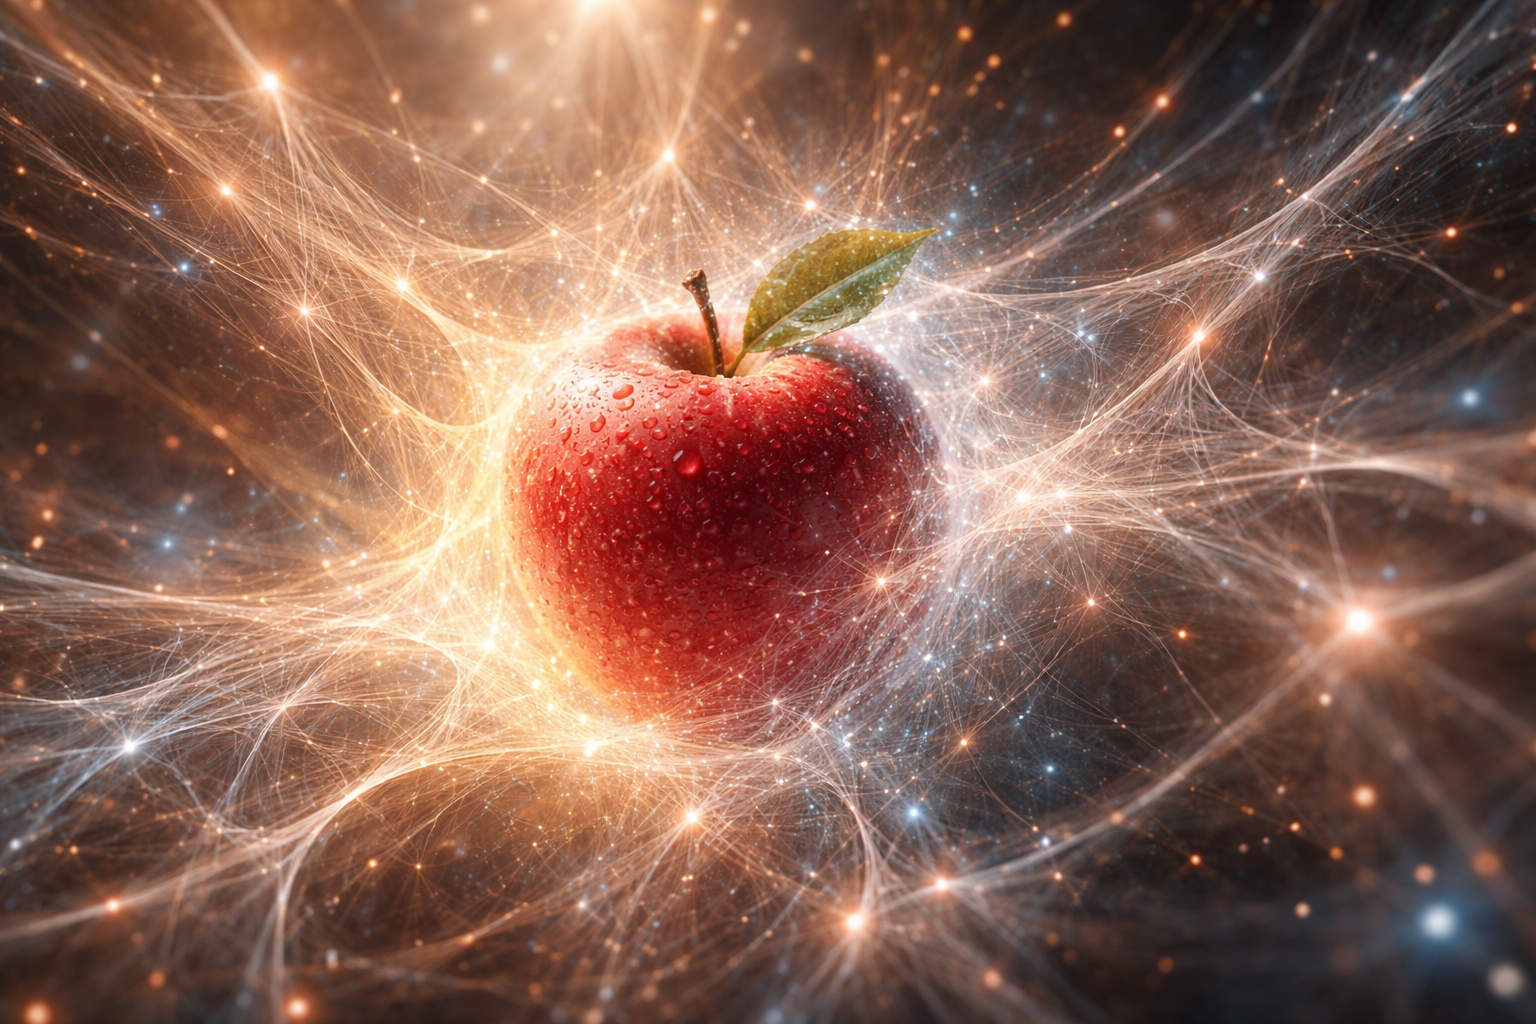
\includegraphics[width=0.82\linewidth,height=0.54\textheight,keepaspectratio]{image/real_apple.png}
\caption{环境对象的观察入口：苹果图像提供外观证据，关系、内部状态与行动结果仍需分别估计。}
\end{figure}

\section{预测、尺度与粗粒化：模型只保留任务所需信息}
\label{sec:condensed_matter}

结构化估计的用途不是建立一份无限细致的对象清单，而是支持指定预测与行动。辨认苹果种类时，颜色和形状可能足够；规划抓取时，还需要位置、接触条件和可用动作；判断长期保存状态时，则需要不同的观测和时间尺度。我们因此先规定任务输出，再讨论表示需要保留哪些信息。同一个环境可以产生多个合适的模型，这些模型不必具有相同维数，也不必以相同关系为核心。

令任务目标为 $y_k$，联合表示为 $x_k=e(o_{0:k},a_{0:k-1})$，读出为 $\widehat y_k=r(x_k)$。经验风险是在指定数据集合上计算的预测损失，而总体风险还依赖任务分布。即使两者的表达形式相似，也不能未经检验便相互替代。我们用训练外的数据、不同观测条件和干预试验检查模型是否保留了所需信息。若目标随任务改变，原先有效的编码可能不再充分。任务相关性不是编码的永久身份，而是编码、读出与评估条件之间的关系。

粗粒化是把多个细节状态映射成一个较简约状态。设 $c:\mathcal Z\to\mathcal C$ 为压缩映射。要使压缩状态独立支持确定性更新，必须存在 $\overline T$ 满足
\begin{equation}
c(T(z,a))=\overline T(c(z),a).
\end{equation}
若两个环境状态被压成同一个状态，但同一动作产生不同的下一压缩状态，便无法在当前压缩变量上定义唯一的更新函数。这个结论直接来自函数的单值性，不需要引入物理类比。遇到这种情况，我们可以细化状态、增加历史记忆或使用条件分布；不能只是把原来的单值预测写得更复杂。

例如，只记录苹果当前位置，可能不足以预测下一时刻位置，因为相同位置可能对应不同速度。加入速度后，在某些模型假设下预测更充分；若动作与接触状态仍未记录，模型还会出现系统性误差。这里的速度属于环境模型的领域变量，其必要性由预测任务决定。内部处理器并不因此必须具有与苹果相同的运动规律。我们把两层描述分开，才可以在保留真实领域约束的同时，为认知更新选择合适的计算实现。

尺度变化也会改变属性的含义。单个对象的局部特征、一个对象集合的统计量与整个场景的任务状态不是同一类变量。集合的平均颜色不能替代每个成员的颜色；场景中的可通行性也不能还原成某个物体的单独属性。我们通过聚合算子明确这些变量怎样形成，并记录聚合所丢失的信息。若使用平均值，应说明权重与样本范围；若使用最大值，应说明它是否代表最危险情况还是最明显证据。聚合方法本身会影响后续决策。

预测误差需要按照用途分解。身份匹配错误、测量误差、压缩损失和转移模型偏差可能产生相同的输出偏差，却需要不同修正。重新训练读出不能必然修复错误身份；增加采样频率也不能消除不合适的状态定义。我们为评估设置分层诊断：固定真实身份检查属性估计，固定属性检查关系推断，再检查整个预测流程。这样才能说明一次改进来自何处，以及它能否迁移到新的任务尺度。

对一般智能而言，重要能力是根据任务重新选择尺度并知道何时细化。系统可以先用简约模型探索，再在误差达到关键阈值时增加变量；也可以在稳定阶段把重复细节聚合为摘要。细化与压缩都应保留接口和证据回溯能力。我们不把更大模型自动视为更深理解，而以任务保持、误差可控和资源可承受作为共同标准。这为后续的状态动力学提供了可以变化但仍有明确意义的模型边界。

\section{领域规律、约束验证与行动闭环}
\label{sec:mirror_table}

环境模型需要服从对应领域的知识，但知识进入模型的方式必须明确。一个机器人抓取苹果，需要考虑尺寸、位置、接触条件和设备限制；一个文本系统整理苹果资料，则可能主要需要来源一致性、术语定义和时间信息。前者可以调用机械模型，后者可以调用文档检查规则。我们不以同一套物理方程解释两个系统的全部内部活动，而是在一般状态接口中容纳各自需要的约束与更新机制。

对连续控制任务，可将可接受状态集合写为 $K=\{z:g_j(z)\leq0,\ j=1,\ldots,m\}$。约束函数可以表达设备工作范围、对象间距或其他领域条件。若模型预测下一状态位于集合中，只说明预测满足模型约束；实际状态还受到模型误差与未记录扰动影响。系统需要为误差保留裕量，并在执行后使用观测校正。把预测可行直接理解为实际必然可行，会把模型边界之外的不确定性藏入动作接口。

在简单标量约束下，我们可以清楚展示误差如何进入决策。设实际值为 $v$，预测值为 $\widehat v$，已验证的误差界为 $|v-\widehat v|\leq\varepsilon$，要求 $v\leq b$。若采用 $\widehat v\leq b-\varepsilon$，则由 $v\leq\widehat v+\varepsilon\leq b$ 得到约束满足。这一推理只在误差界有效的条件下成立。更复杂约束需要相应的敏感性界，不能把同一个标量裕量无条件套到所有变量上。我们在公式旁说明误差界来自何处、在哪些条件下失效。

行动闭环由估计、预测、选择、执行和再观测组成。选择动作前，系统检查当前对象身份、模型版本和所需资源；执行后，系统比较预期与实际记录。若差异显著，应先判断差异是测量异常、动作未执行、环境变化还是模型错误，再决定是否继续。一个指令被生成，不等于它已经执行；工具返回成功，也不一定等于预定环境结果已经出现。我们用不同事件记录这几个阶段，以免认知状态抢先宣告任务完成。

证据不充分时，主动测量本身可以成为动作。苹果是否已经被抓住，可能需要夹持反馈或新的图像；资料中的日期冲突，则可能需要读取原始记录。我们可以比较不同测量动作预计减少的不确定性和所需成本，但成本函数必须符合当前任务，不能把所有计算、时间与错误风险不加解释地压成一个数。若采用加权和，权重表达决策偏好，其来源和调整规则也应成为模型的一部分。

领域知识还需要版本与适用条件。机械模型可能只在某个速度范围和接触类型下有效；分类模型可能只覆盖规定类别；文档规则可能依据某个时间版本。内部系统应保存这些条件，使超出范围的输入触发重新评估。通过这种机制，约束不是一段永远正确的声明，而是与数据、动作和验证流程相连的可执行知识。发现违反条件时，系统可以收缩行动范围、追加观测或切换模型。

本章所建立的环境对应关系，最终可以进入 AgentOS 的对象记录、工具接口与事件日志。HSF-HD 在这里规定一般的状态组织和更新要求，而具体传感器、机械方程或文档工具属于实现层。我们评价一个实现时，应同时检查任务效果、证据可回溯性以及更新规则是否在所声明条件下运行。环境可以非常复杂，但有效智能并不需要先宣称已经复制整个环境；它需要形成足够可靠、能够被校正且能支持行动的局部模型。

\chapter{认知对象的结构化表示：语言、视觉与关系}
\label{chp:semantic_anatomy}

环境记录进入系统之后，还需要被组织成可以用于判断、推理和交流的认知对象。我们用这个名称指系统内具有身份、属性和关系的表示单位，不预设它与主观体验等同，也不要求它复制外部对象的全部细节。一个句子、一幅场景图和一条论证链都可以包含这些单位，但它们的关系规则不同。语言中的施事角色不能直接当作图像中的左侧位置，逻辑蕴含也不能直接当作事件因果。本章分别说明语言、视觉和推理中的结构内容绑定，再讨论它们怎样通过明确接口协作。我们把理解表述为一种任务能力：系统能够在语境变化下维持对象与关系，回答有证据支持的问题，并依据新信息修订原有解释。这样，认知对象的有效性可以接受检查，而不依赖向量外观、几何修辞或输出流畅程度来证明。

\section{语言表示：表达顺序、事件角色与语境消歧}
\label{sec:language_structure}

语言输入以字符、词项或其他符号序列出现，但序列顺序并不足以表达所有关系。“猫追鱼”和“鱼追猫”具有相同的对象词与动作词，事件角色却相反。如果系统只保存词项出现次数，就无法回答谁是追逐者。我们因此把表面序列、句法依赖和事件角色作为不同层次的记录。它们可以相互支持，也可能彼此不一致。错误输入、歧义表达和省略现象都要求系统保留候选解释，而不是从词序直接跳到唯一事件。

设事件 $e$ 具有动作类型和若干角色槽位，我们用 $R(e,\mathrm{actor},i)$ 与 $R(e,\mathrm{target},j)$ 记录施事和目标。这些关系包含角色类型，交换对象身份会改变事件内容。若用上一篇的张量绑定形式，可写为 $T_e=\sum_r v_r q_{e,r}^{\mathsf T}$，其中 $v_r$ 是角色编码，$q_{e,r}$ 是角色内容。角色编码必须满足读出所要求的可区分条件；否则，施事与目标可能在压缩后混淆。公式提供一种实现，但事件角色的语义来自建模规范和验证任务，不能从张量乘法本身产生。

词义需要语境。一个词项可能表示物体、动作或某个专业概念；相同词项在不同语境下的读出不应被强行固定。我们将词项的基础编码与上下文更新后的对象表示区分，要求上下文更新保存与任务相关的身份信息。例如，“把它放在桌上”中的代词需要指向已有对象；若前文出现多个候选，“它”的归属应由对话条件和任务证据决定。系统可以请求或寻找更多证据，也可以明确保留分支，而不应把最高相似度候选当成已证实身份。

语法可接受与事实正确是两个不同检查。一个句子可以结构完整却与环境记录冲突，也可以表达想象情境而没有声称其为现实。我们在认知对象中保留表达模式：事实陈述、条件假设、引用内容与反事实推演不能混为一谈。对“假如苹果是蓝色的”进行推理，不要求系统把现实苹果的颜色改成蓝色；它要求建立受条件约束的分支表示。分支结束后，事实状态仍应由原始证据支持。这种作用域管理是理解复杂语言的必要组成部分。

语义冲突也不是简单的向量相反。两个描述是否冲突，取决于对象身份、时间、属性定义和语境。苹果在昨天为青色、今天变为黄色，未必矛盾；两个来源在同一条件下给出互斥类别，才构成需要解释的冲突。我们把冲突检查落实到这些字段，并记录当前的解决依据。仅在编码空间中计算夹角，可能有助于发现候选冲突，却不能代替类型、作用域和证据条件的检查。

语言理解的评估应覆盖关系干预。我们可以保持词项不变而交换角色，检查回答是否随角色改变；可以改写表达而保留事件，检查关键读出是否保持；还可以加入无关句子，检查原对象身份是否稳定。三个试验分别检查关系敏感性、表达稳健性和干扰控制。单一问答正确率很难区分这几种能力。尤其当系统记住常见搭配时，它可能回答原句，却无法处理角色互换后的句子。

在持续对话中，新输入不仅添加内容，还可能修订旧对象。用户说明“我刚才说的苹果其实是模型道具”，系统应调整对象类别、可用属性和相关推理，而不只是追加一句备注。我们保存修订事件及其影响范围，使仍依赖旧解释的计划进入重新检查。语言表示由此成为能够维护的任务状态，而非输入文本的静态摘要。HSF-HD 在这一层提供一般的绑定、作用域与修订要求，具体语言模型只是完成这些操作的一种实现选择。

\section{视觉表示：区域、对象身份与场景关系}
\label{sec:vision_structure}

视觉输入首先是由采样装置产生的数组。对象、轮廓和空间关系需要从数组中估计，而不是直接写在像素里。同一个对象可以因视角改变而呈现不同区域，两个不同对象也可能具有相似外观。我们将区域记录、对象记录和场景关系分开：区域指向当前图像位置，对象维持跨时刻身份，关系则说明对象之间的相对组织。这样，移动对象不必改变其身份，摄像机移动也不必被解释成所有对象都改变了位置。

区域记录可以包括边界框、掩码和可见性标记。对象属性则可以包含类别候选、外观编码与估计尺度。边界框通常只是一种位置摘要，不能精确代表对象占据的全部区域；掩码表达更细的像素归属，但仍可能受到遮挡影响。我们不把检测输出当成无误的对象定义，而是保存算法版本与支持证据。当任务要求接触位置时，分类准确并不足够，还需要相应的几何估计与误差范围。

场景关系需要声明坐标系与尺度。“苹果在盘的左边”可能依据图像坐标，也可能依据操作者视角；更换视角后，同一句关系可能改变。包含、接触与遮挡又具有不同含义。遮挡关系主要表达某个观测视角下的可见性顺序，不能自动推出物体之间的接触关系。我们为关系添加参照系与观测条件，使同一场景中不同来源的关系能够被比较，而不是仅凭相同标签合并。

对象追踪使用跨帧证据维持身份。若两个外观相似的苹果交叉移动，系统可能暂时无法确定对应关系。我们可以把匹配表示为带约束的候选分配，要求一个观测候选不同时归属两个互斥对象；遇到遮挡、合并或分裂时，则需要显式事件更新。只有在证据足够时，才把候选匹配提交为新的身份关系。身份错误会传播到历史轨迹与动作计划，因此它应拥有独立于类别置信度的诊断指标。

结构与外观可以相互帮助，但这种帮助不能替代证据。例如，盘的边缘可能帮助解释被遮挡苹果的轮廓；同时，苹果的形状也能帮助判断哪条边属于盘。系统在联合估计中可以使用先验形状，但必须区分直接可见区域与补全区域。补全结果可能对预测有用，却不是新增观测。若把推断出的边界标记为已观测，后续系统就可能高估确定性，并在新的视角出现时拒绝合理修订。

我们可以通过控制结构与属性的变化检查表示分工。保持位置关系而改变颜色，适合检查对象定位是否依赖不必要的外观捷径；保持外观而交换对象位置，适合检查场景关系是否真正编码。评价这些试验时，应同时考察对象身份、关系读出和任务结果。仅凭重建图像相似，无法证明内部状态保留了所有关键关系，因为重建目标可能更关注像素而非角色和对象连续性。

视觉与语言的对齐需要对应对象，而不只是对应整体句子与整体图像。“盘里有两个苹果”要求语言中的数量、包含关系和对象类别都能在视觉记录中找到支持。若某个苹果被遮挡，系统应说明数量是直接数得、由历史追踪维持还是由模型推断。跨模态接口由此不仅传递编码，还传递证据条件。对于 AgentOS，这使视觉工具的结果能够参与可回溯的任务状态，而不会仅以一段自然语言描述取代所有原始依据。

\begin{figure}[htbp]
\centering
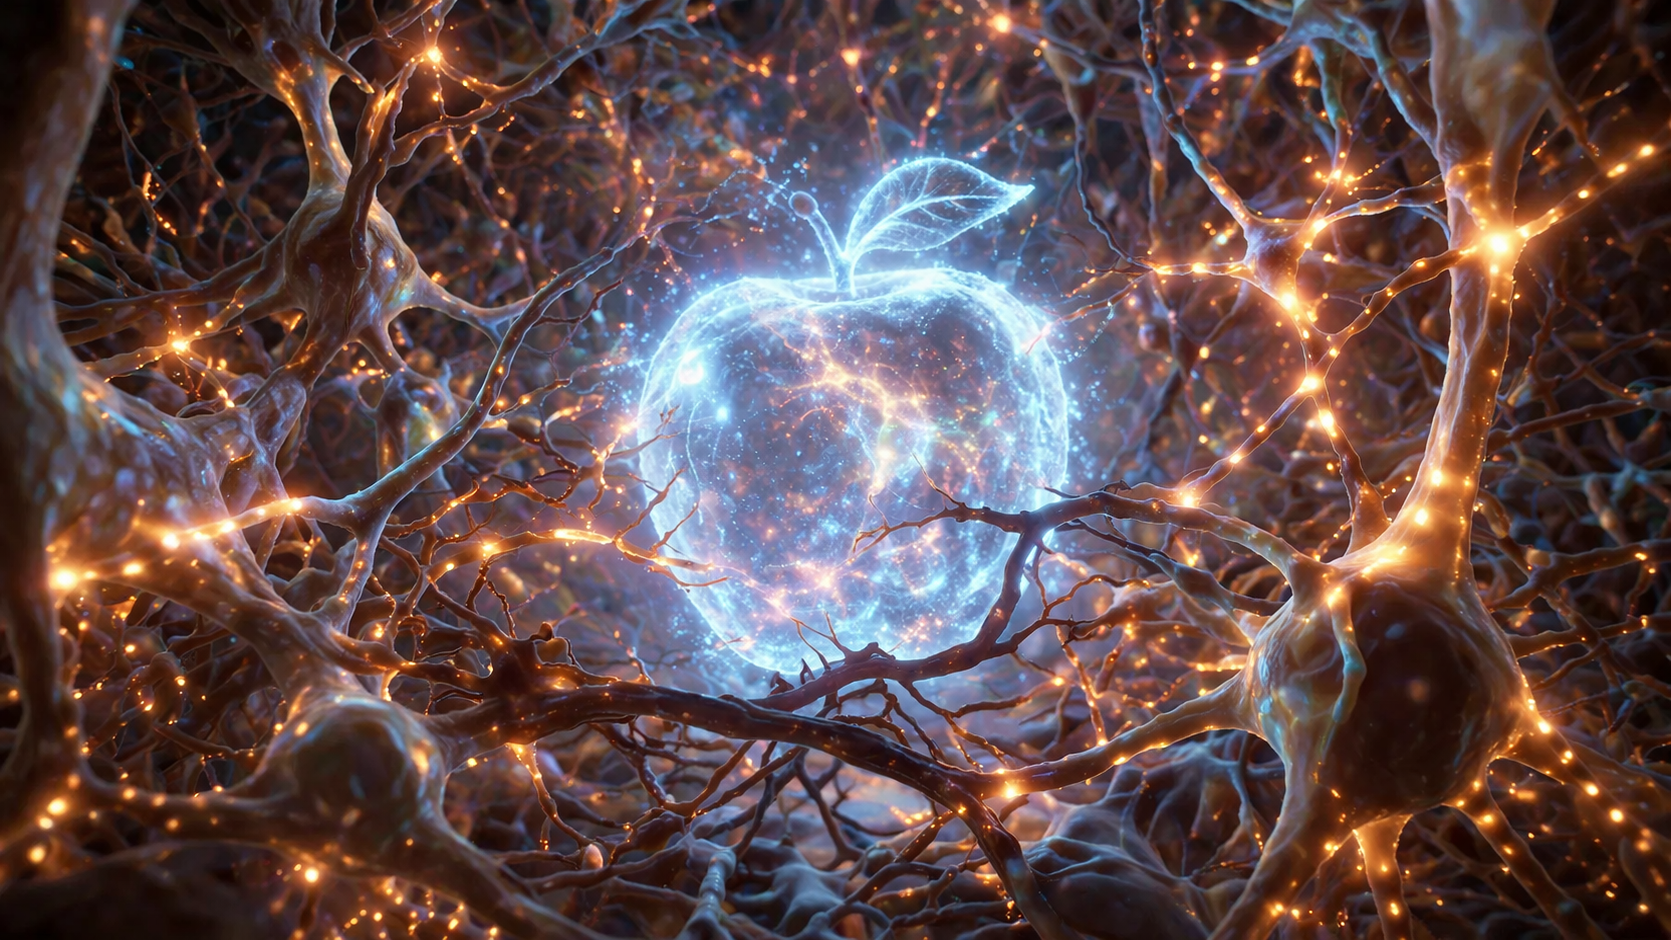
\includegraphics[width=0.82\linewidth,height=0.54\textheight,keepaspectratio]{image/nureal_apple.png}
\caption{苹果的内部表示示意：对象、属性与关系属于系统组织的任务状态，其有效性需由观测和读出分别检验。}
\end{figure}

\section{推理表示：证明依赖、可信程度与因果条件}
\label{sec:logic_structure}

推理需要在对象之间建立可检查的依赖。我们首先区分形式蕴含、统计相关和环境因果。形式蕴含要求结论依据规定推导规则从前提产生；统计相关描述变量在某个分布下共同变化；因果关系还涉及干预以及对干预后结果的预测。这三种关系可能在同一任务中相互协作，却不能用同一条无类型边代替。一个图上存在连通路径，也不足以说明沿路推导有效，因为路径中的关系类型和条件可能不兼容。

以命题逻辑中的一次推导为例，前提集合包含 $A$ 和 $A\Rightarrow B$，使用规定规则得到 $B$。我们记录结论节点、前提节点及所用规则，形成一个证明事件。检查器需要验证该事件的输入类型、作用域和规则实例，而不是只检查节点相邻。若前提位于一个暂时假设分支，结论也继承该分支条件；离开分支时，不能把结论直接当成无条件事实。证明依赖图因此既记录推导顺序，也记录成立条件。

命题真值与系统可信程度不能混淆。某个命题在指定语义下为真，并不意味着系统已经有充足证据知道它为真；反过来，高置信度判断也可能错误。我们分别保存形式检查结果与经验支持。概率推断要求联合分布或相应的条件独立假设，不能把两条前提置信度随意相乘来获得结论概率。若缺少这些条件，系统应使用有明确意义的评分或区间，而不把结果包装成精确概率。

依赖记录使撤回成为可计算操作。若前提 $A$ 的证据失效，所有仅依赖该证据的结论需要重新评估；若某个结论还有独立证明，则不能简单一并删除。我们为结论保存多个支持集合，在修订时检查是否仍存在有效支持。这个机制比一句“更新信念”更具体，因为它规定了什么发生变化、哪些结果受到影响，以及为何某些结果仍被保留。复杂任务中的一致性维护依赖这样的结构。

因果推理还需要区别观察条件与干预条件。看到某变量与另一变量共同变化，只能提供相关证据；主动改变前者后，后者是否随之变化，取决于系统机制和其他条件。我们可以用类型化接口分别记录观测分布与干预预测，并要求模型声明它们之间的连接假设。对无干预能力的任务，也可以提出因果候选，但应保留其证据限制。语言表达中的“因为”不是自动成立的因果证明。

寻找证明与检查给定证明也是不同计算任务。某些问题中，给定见证可以较快检查，而寻找见证需要大量搜索；这种差异依赖问题类型和表示方式，不能被宣称为所有推理的普遍成本定律。我们在任务记录中分别统计候选生成成本、检查成本和失败回溯成本。生成模型可以提出辅助条件或新候选，检查器则判断候选是否满足规则。创造性探索与严格验证因而可以协作，无须把探索禁止后才能获得可靠推理。

推理的状态更新包括增加前提、提交已验证步骤、保留未验证候选与撤回失效结论。每种更新都有不同条件。我们不把所有认知内容压成一个持续增大的真值列表，而是维护具有状态和来源的论证对象。对于 AgentOS，一个规划建议、一次工具结果和一条经检查的推导可以共享记录接口，却需要不同的有效性标记。HSF-HD 所提供的一般性在于规定依赖与更新的组织方式，而不是把所有知识都化约成同一种推理规则。

\section{跨模态协作：共同身份、接口契约与可修订理解}

语言、视觉和推理可以协作，是因为它们能够建立任务相关的对应关系，而不是因为它们天然拥有相同编码。我们首先定义共同身份接口：语言中的“这个苹果”、视觉追踪中的目标对象和规划中的操作对象，需要指向同一个任务实体或明确的候选集合。身份接口不要求三个模块保存同一个向量，但要求它们能够解释何种证据支持对应，以及对应失败时怎样修订。

接口契约规定输入类型、输出类型、有效条件与错误状态。视觉模块可以输出区域候选和对象属性，语言模块可以输出事件角色与指代候选，推理模块可以输出检查结果与依赖关系。接收方不能凭字段名字相似便认定语义一致。例如，视觉置信度可能是分类评分，语言置信度可能是生成评分，两者没有共同校准依据时不应直接平均。我们可以通过统一任务上的校准或选择规则组合它们，但必须说明组合目标。

在数值消息传递中，设对象 $i$ 的状态为 $x_i^k\in\mathbb R^d$，关系类型为 $r$，更新可以采用
\begin{equation}
x_i^{k+1}=f\left(x_i^k,\sum_r\sum_{j\in\mathcal N_r(i)}A_r x_j^k,u_i^k\right).
\end{equation}
矩阵 $A_r$ 把对应消息映射到共同消息空间，加和因此具有明确类型；函数 $f$ 再产生下一状态。这个机制能够表达关系敏感更新，却不保证自动完成逻辑证明或对象追踪。关系是否被正确建立、消息是否保留关键角色以及读出是否满足任务条件，仍需要独立验证。数值运算的可微性不等于语义正确性。

理解可以通过一组任务能力得到操作化描述。系统需要回答直接问题、处理等义改写、识别角色交换、解释来源冲突，并在新证据出现时修订判断。这些能力共同构成一个评估范围，任何单项成功都不必然推出其余能力。我们还检查更新后的状态是否保持旧任务中仍然有效的关系，避免新信息覆盖对象身份或作用域。持续任务中的理解，因此不仅表现为当前输出，还表现为修订过程是否保存了必要连续性。

以“拿起盘中较大的苹果”为例，语言解析需要给出操作类型、目标限定与比较属性；视觉处理需要定位盘、建立包含候选并估计大小；规划需要选择可行抓取动作。若两个苹果大小相近且误差区间重叠，系统应保留选择不确定性，必要时获取新的视角。若用户随后说明“我指的是左边那个”，这条输入修订目标限定，但不必改变两个苹果原有的视觉身份。各模块通过共同实体和修订事件协调，才不会把新增限定误当成新增对象。

跨模态冲突不应总由某个模块固定裁决。语言可能提供视觉无法看到的属性，视觉也可能纠正语言中的旧描述，形式检查则可能揭示两者联合时的作用域错误。我们根据证据类型、时间和任务要求选择裁决方式，并保存无法解决的冲突。系统可以暂停依赖该冲突的行动，同时继续与其无关的工作。这种局部阻断比让一个不确定判断污染全部任务状态更有利于维持持续运行。

我们最终把认知对象看作可组织、可读出和可修订的计算状态。它们的内容可以来自多种输入，其关系必须具有明确含义，其更新需要保留证据与依赖。这个定义为一般智能理论提供了共同接口，同时保留不同模态和推理机制的差异。AgentOS 可以在这一接口上实现工具协作、任务记忆与执行记录；它的具体模块并不是 HSF-HD 一般理论的前提，而是对一般状态组织要求的一种工程实现。

\chapter{领域表示的异构性：任务尺度与跨域接口}
\label{chp:domain_manifolds_heterogeneity}
% Legacy section labels temporarily resolve to the chapter.
\label{sec:manifold_of_language}
\label{sec:manifold_of_logic}
\label{sec:manifold_of_physics}
\label{sec:manifold_of_biochem}
\label{sec:manifold_of_society}
\label{sec:manifold_of_industry}
\label{sec:topological_shapeshifter}
我们将不同领域视为具有不同变量、关系、时间尺度和观测限制的模型空间。通用性来自可组合接口与适应机制，不来自强行采用同一表示。
\section{领域状态与局部适用性}
令领域 $d$ 的状态为 $x_d\in\mathcal X_d$，更新为 $x_d^+=F_d(x_d,u_d)$。文本、场景图、程序状态和运动控制可能分别采用序列、图、离散状态机与连续向量。每种空间具有自己的合法操作和约束。
\section{跨域映射与误差}
映射 $E_{ab}:\mathcal X_a\to\mathcal X_b$ 应声明任务相关的保真量。我们可以检验转移的一致性误差
\begin{equation}\delta_{ab}(x,u)=d_b\left(E_{ab}(F_a(x,u)),F_b(E_{ab}(x),U_{ab}(u))\right),\end{equation}
其中 $U_{ab}$ 转换输入，$d_b$ 是目标域的指定距离。两域操作维度不同或信息不足时，误差可能无法消除。任务相关的近似对应不等同于整个领域之间的严格同构。
\section{多尺度接口与调度}
局部控制、语义推演和长期规划具有不同截止时间。接口需要规定采样率、最大延迟、误差预算和失败后的处理方式。低频过程可以施加持久约束，但其影响范围必须由架构和耦合通道确定，不能由低频本身推出。

\chapter{环境与认知的结构对应：可观测性与近似等价}
\label{chp:holomorphic_isomorphism}
% Compatibility anchors: old section references resolve to this chapter.
\label{sec:brain_cosmos}
\label{sec:holomorphic_theorem}
\label{sec:comprehensibility}
\label{sec:godel_gap}

我们将环境与内部模型的关系表述为任务相关的结构对应。预测性能可以约束内部表示，但不能单独证明内部空间与整个环境同胚。
\section{任务相关的等价类}
令环境状态为 $z$，允许的动作和观测历史共同确定任务。若两状态在所有允许策略下产生相同的未来任务观测分布，我们将它们记为 $z\sim z'$。这个等价关系依赖任务、传感器和可用干预；改变这些条件后，原等价类可能需要细分。
\section{动力学映射的定义}
考虑确定性特例 $z_{k+1}=T(z_k,a_k)$，内部状态 $x=e(z)$，内部预测转移为 $\widehat T$。严格对应要求
\begin{equation}e(T(z,a))=\widehat T(e(z),a).\end{equation}
这是转移的交换关系。如果 $e$ 非单射，它至多构成任务相关的压缩映射；只有补充双射、逆映射的连续性等条件，才能讨论同胚。随机系统须比较转移核而非单个状态点。
\section{近似误差的传播}
设编码域内的一步误差不超过 $\delta$，$\widehat T$ 对状态为 $L$-Lipschitz，且比较轨迹使用同一动作序列。令 $E_k=\|e(z_k)-x_k\|$，三角不等式给出 $E_{k+1}\le\delta+LE_k$。若 $E_0=0$，则
\begin{equation}E_k\le\delta\sum_{j=0}^{k-1}L^j.\end{equation}
当 $L<1$ 时误差有统一上界；$L\ge1$ 时长期误差可能增长。闭环动作随内部预测改变时，还需计入策略敏感性。本书据此将结构对应视为有条件、可测量的模型性质。

\section{表示与示意图}
我们保留以下示意图以展示原有结构关系。图中历史物理术语遵循阅读约定中的计算解释；图的形式相似性不代替本章的假设、推导和验证。
\begin{figure}
\centering
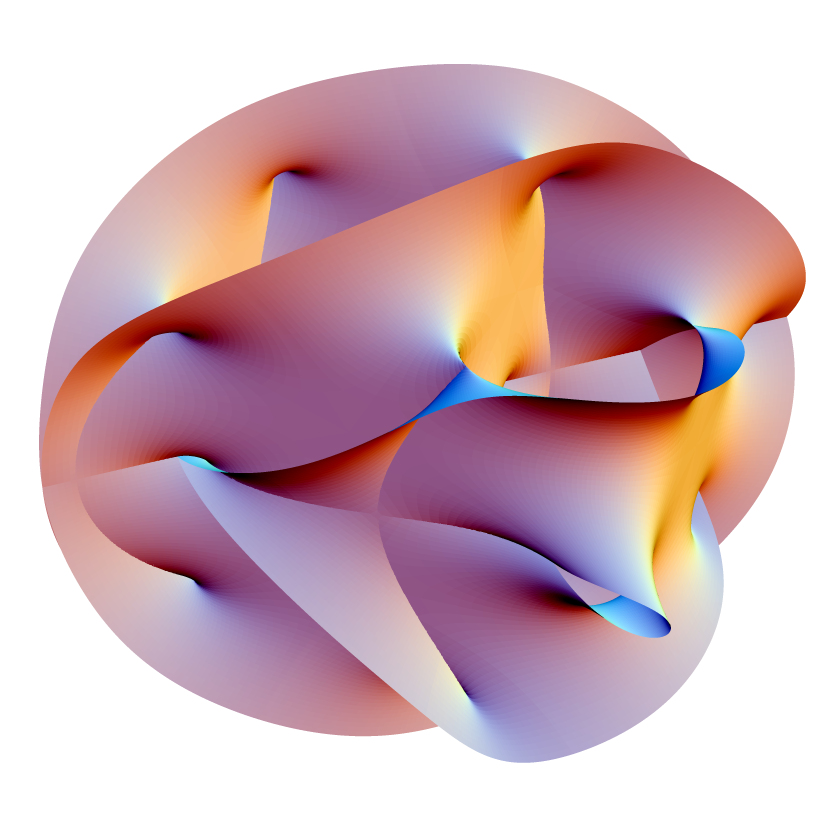
\includegraphics[width=0.4\textwidth]{image/Calabi.png}
\caption{一种流形结构}
\end{figure}


\chapter{MST 架构：结构与内容的联合注意力}
\label{chp:mst_architecture}
% Legacy section labels temporarily resolve to the chapter.
\label{sec:dual_encoder}
\label{sec:fusion_attention}
\label{sec:hybrid_decoder}
\label{sec:mst_complete}
\label{sec:training_paradigm}
我们提出形质联合 Transformer（MST）作为结构与属性分解的一种工程实例。架构假设必须通过实验检验，它不是 HSF-HD 唯一可能的实现。
\section{双通道与类型约束}
设输入包含 $n$ 个对齐位置，结构通道为 $T\in\mathbb R^{n\times d_s}$，内容通道为 $X\in\mathbb R^{n\times d_x}$。两通道可以使用不同编码器，但位置对应关系必须由数据或对齐模块定义。未经对齐的两个序列不能直接按同一节点索引融合。
\section{结构引导的内容聚合}
取 $Q=TW_Q$、$K=XW_K$、$V=XW_V$，其中 $Q,K\in\mathbb R^{n\times d_k}$，$V\in\mathbb R^{n\times d_v}$。定义
\begin{equation}A=\operatorname{softmax}_{row}\left(\frac{QK^\top}{\sqrt{d_k}}+M(S)\right),\qquad Z=AV.\end{equation}
掩码 $M(S)$ 表示允许关系，不允许的边可设为负无穷。每一行至少有一个合法位置，才能避免归一化未定义。$A$ 是聚合权重，不是结构与内容在物理意义上的纠缠。
\section{目标与训练}
给定结构目标 $S^*$、属性目标 $X^*$ 和任务目标 $y$，可以定义
\begin{equation}\mathcal L=\lambda_s\ell_s(\widehat S,S^*)+\lambda_x\ell_x(\widehat X,X^*)+\lambda_y\ell_y(r(Z),y)+\lambda_b\ell_b(T,X).\end{equation}
绑定损失 $\ell_b$ 的正负样本需要符合任务语义；错误的负样本会惩罚合法组合。不同损失项应按尺度设置权重，训练损失下降不保证分解可辨识或域外泛化。
\section{复杂度与对照实验}
稠密 $QK^\top$ 仍具有二次交互成本。稀疏关系可以减少实际交互数量，但必须说明稀疏模式和实现。我们以单通道基线、双通道无绑定、关系扰动和跨域测试区分结构分解带来的收益与参数增加带来的收益。

\chapter{结构化生成：从输入描述到可执行结果}
\label{chp:generative_creation}

上一章建立了结构位置与内容记录之间的联合注意力，本章进一步追问：当系统收到一句自然语言、一个观测样本或一段持续任务说明时，怎样把条件表示变成可以检查、修订和执行的结果？我们把生成理解为受约束的状态构造过程，而不是把语义“物质化”的神秘跃迁。生成器必须同时维护对象身份、关系、属性、时间版本与读出接口；任一层发生改变，相关约束和评价指标都应随之更新。文本到图像、图像到文本和视频生成只是这一模型族的三个实例，它们不能代表全部智能，也不能仅凭输出逼真度证明系统已经理解世界。我们将以“红苹果位于木桌上”这一旧例贯穿推导，并把理型、范畴和现象学的历史讨论改写为关于不变量、架构先验与交互可辨识性的计算问题。由此，HSF-HD 所研究的是一般智能状态如何在条件、约束与反馈下演化；MST 是一种联合表示部件，而 AgentOS 才是在具体工程中组织记忆、调度、边界和外部执行的实例。

\section{条件生成：从描述解析到结构化读出}
\label{sec:text_image_msc}

我们先定义生成问题的对象。设输入描述为 $u\in\mathcal U$，解析器输出带类型的需求记录 $R(u)=(V_u,E_u,A_u,C_u)$：$V_u$ 是对象声明集合，$E_u$ 是关系声明集合，$A_u$ 是按对象身份索引的属性集合，$C_u$ 是显式约束与未决条件集合。对于“一只红苹果放在木桌上”，对象不是两个无来源的向量，而是带稳定标识的 $v_a=\langle\texttt{apple},\texttt{id}=a\rangle$ 与 $v_t=\langle\texttt{table},\texttt{id}=t\rangle$；关系是 $\texttt{on}(a,t)$，属性是 $\texttt{color}(a)=\texttt{red}$ 与 $\texttt{material}(t)=\texttt{wood}$。语句没有给出桌面尺寸、视角、光照和精细形状，这些都必须标记为缺省变量或待采样变量，不能在解析阶段伪装成已经由文本确定的事实。否定、量词、指代和歧义也要进入记录，例如“不是红桌子”约束的是属性绑定，而不是简单删除词向量。

生成状态记为 $Y=(G,X,Z,M)$。其中 $G=(V,E)$ 是离散结构图，$X\in\mathbb R^{n\times d_x}$ 是与 $n$ 个结构位置对齐的连续属性，$Z$ 是面向具体读出器的潜在表示，$M$ 保存身份、来源、置信区间、单位和版本。这里的数值没有默认物理单位：像素坐标可用归一化图像单位，三维场景坐标必须声明长度单位，颜色可以位于规定色域，置信度才位于 $[0,1]$。我们定义合法集合
\begin{equation}
  \mathcal C(u)=\{Y:\;c_j(Y,R(u))\le 0,\ j=1,\ldots,J,\quad e_k(Y,R(u))=0,\ k=1,\ldots,K\},
\end{equation}
其中不等式可表达边界、遮挡预算或最小间距，等式可表达身份绑定和确定关系。若 $\mathcal C(u)=\varnothing$，正确行为是报告冲突并返回最小冲突集，而不是生成一张看似合理却违背输入的图像。比如同时要求苹果完全位于桌面上、苹果直径大于桌面宽度且不允许悬垂，在给定几何模型下可能不可行；系统应指出是哪三项约束共同导致不可行。

在合法集合非空时，我们把候选构造写为
\begin{equation}
  Y^*\in\arg\min_{Y\in\mathcal C(u)}
  \mathcal J(Y;u)=\lambda_r L_{\mathrm{req}}+\lambda_s L_{\mathrm{struct}}
  +\lambda_a L_{\mathrm{attr}}+\lambda_q L_{\mathrm{readout}},
\end{equation}
各损失先分别无量纲化，权重 $\lambda_\bullet\ge0$ 才能比较。$L_{\mathrm{req}}$ 衡量显式要求是否满足，$L_{\mathrm{struct}}$ 衡量关系与布局冲突，$L_{\mathrm{attr}}$ 衡量属性绑定，$L_{\mathrm{readout}}$ 衡量输出域质量。这个式子是工程目标定义，不保证极小点唯一，也不意味着目标下降必然带来用户任务成功。离散图编辑与连续属性优化可以交替进行，但每次图结构改变后，目标的定义域、掩码和候选集合都可能改变；只有在同一目标、同一约束集并且每一步确实不增目标的条件下，才能声称目标序列单调。

从描述到图像时，结构读出器先把 $G$ 与 $X$ 转为布局、深度、遮挡顺序和区域身份，再由渲染读出器 $D_{\mathrm{img}}(Y,\xi)$ 产生图像，$\xi$ 表示视角、随机种子和渲染配置。旧叙述中的“先造骨、后填肉”在这里仅表示一种模块化计算顺序：先确定任务相关的关系支持，再将属性绑定到身份明确的位置，最后读出。它不是关于世界本体的断言，也不要求所有生成系统都采用双塔。端到端扩散模型同样可以通过交叉注意力、控制网络、显式布局或采样校正满足结构条件；结构化方案的优势必须以关系准确率、属性绑定错误率、可编辑性和失败报告质量来检验，不能用“构造优于概率”作先验结论。

对于苹果例，最小验收集合至少包括：苹果身份在所有中间状态中不与桌子交换；红色绑定到苹果而非桌子；$\texttt{on}(a,t)$ 被操作化为接触或支撑关系，而不是仅比较二维纵坐标；改变苹果颜色时桌面材质保持不变；改变视角时对象身份和三维关系保持一致。生成一幅漂亮图像只验证读出结果的一次样本，不能验证内部图与真实场景严格同构。结构状态应作为可检查的中间产物返回，使人或后续程序能够修改 $G$、$X$ 或 $C_u$ 后重算，而不是只能反复改写提示词。

\begin{table}[htbp]
  \centering
  \caption{两类实现路线的可检验差异，而非本体优劣}
  \label{tab:sd-vs-msc}
  \begin{tabular}{@{}p{0.17\textwidth}p{0.36\textwidth}p{0.39\textwidth}@{}}
    \toprule
    \textbf{比较项} & \textbf{隐式条件生成} & \textbf{显式结构化生成} \\
    \midrule
    条件承载 & 条件分布与潜变量中隐式编码 & 类型图、属性表与连续状态共同承载 \\
    局部修改 & 依赖重采样或额外控制模块 & 可在身份与约束不变时编辑指定字段 \\
    失败可见性 & 常需从最终样本反推原因 & 可分别报告解析、可行性、绑定和读出失败 \\
    正确性边界 & 高样本质量不蕴含关系正确 & 中间结构正确也不蕴含最终感知质量 \\
    \bottomrule
  \end{tabular}
\end{table}

\section{逆向生成：从观测分解到有依据的描述}
\label{sec:image_text_msc}

图像到文本不是前一过程的数学逆函数。一个二维观测可以由许多三维场景、光照条件和相机参数产生，遮挡区域更没有唯一解，因此从图像 $I$ 恢复场景状态是欠定推断。我们令观测 $o\in\mathcal O$，候选隐状态仍写为 $Y=(G,X,Z,M)$，观测模型为 $p_\phi(o\mid Y)$，先验或任务约束为 $p(Y\mid c)$。在模型假设成立时，后验满足
\begin{equation}
  p(Y\mid o,c)=\frac{p_\phi(o\mid Y)p(Y\mid c)}
  {\int_{\mathcal Y}p_\phi(o\mid \widetilde Y)p(\widetilde Y\mid c)\,d\widetilde Y}.
\end{equation}
若 $Y$ 同时包含离散图和连续变量，分母应理解为对离散候选求和、对连续分量积分。公式说明描述来自证据与先验的联合，而不是把像素“退相干”为唯一真相。实际系统可以用检测器、分割器、深度估计器和关系头近似这一后验，但每个部件都带有训练分布、传感器分辨率与标注体系的限制。

我们将输出分为观测事实、模型推断和未决项。观测事实是能够从当前输入直接定位的区域、边缘、颜色统计或时间变化；模型推断包括“该区域是苹果”“桌面支撑苹果”和“材质是木质”；未决项包括被遮挡背面、真实质量、内部结构与图像外事件。元数据 $M$ 为每条陈述保存证据索引 $e_i$、来源模型 $s_i$、置信度 $q_i$ 和版本 $v_i$。文本解码器只能使用获得授权的记录集合，句子中的名词、属性和关系必须回指相同身份。例如形状检测认为区域 $r_1$ 是圆形物体，颜色模块在 $r_1$ 上检测到红色，而分类器认为 $r_1$ 可能是苹果或红球，则合理描述是“桌上有一个红色圆形物体，模型更倾向于苹果”，而不是把最高分标签写成无条件事实。

局部结构网络与全局分布表示在这里承担不同作用。场景图保存对象身份、空间邻接、支撑和遮挡等离散关系，便于检查组合约束；全局向量保存风格、整体语境和难以逐项命名的统计特征，便于召回相似经验与生成连贯语言。二者并非脑区映射，也不是互相排斥的两种智能。联合接口需要任务相关身份矩阵 $B\in\{0,1\}^{n\times m}$ 或软绑定 $B\in[0,1]^{n\times m}$，把 $n$ 个图节点与 $m$ 个区域记录关联起来。若采用软绑定，应规定行归一化或允许“无匹配”槽位；若同一纹理区域可能覆盖多个节点，也不能强制列唯一。全局上下文可以调整候选概率，却不应无证据地创造局部对象。

描述生成可写为带证据约束的序列模型。设第 $t$ 个词元为 $w_t$，已生成前缀为 $w_{<t}$，允许使用的证据集合为 $E_t$，则
\begin{equation}
  p(w_t\mid w_{<t},Y,o)=\operatorname{softmax}
  \bigl(\ell_t+\mu A_t(Y,E_t)\bigr),
\end{equation}
$\ell_t\in\mathbb R^{|\mathcal V|}$ 是语言模型日志值，$A_t$ 是同维的证据许可或偏置，$\mu$ 是无量纲控制系数。硬许可可以把没有证据支撑的专名、数量或关系置为不可选，软偏置则只改变概率。注意力权重本身既不是证据概率，也不是因果解释；系统需要另外记录某项陈述由哪些检测结果与规则支持。解码后还要进行身份一致性检查、数值范围检查和关系闭包检查，避免前句称“一只苹果”、后句又把同一身份写成“两只水果”。

评价也应分层。对象和关系可用精确率、召回率与校准误差，属性绑定可用身份条件准确率，语言可读性可由人工或任务指标评价，幻觉率则统计无证据陈述。单一相似度分数容易把流畅但错误的描述与简短而可靠的描述混在一起。反例尤其重要：镜面反射可能造成重复对象，红色照明可能使木桌看似红色，二维重叠不一定表示接触，训练集中“香蕉—黄色”的高相关也不能排除青香蕉。只有在这些干扰条件下仍能维持来源、身份和不确定性，逆向生成才称得上有依据的状态估计。

\section{时序生成：身份、属性与结构事件的联合演化}
\label{sec:video_generation}

视频生成把单次构造扩展为时序状态转移。我们在离散时刻 $t_k=k\Delta t$ 定义状态 $Y_k=(G_k,X_k,Q_k,M_k)$：$G_k$ 是当时有效的对象—关系图，$X_k\in\mathbb R^{n_k\times d_x}$ 是位置、姿态和其他连续状态，$Q_k\in\mathbb R^{n_k\times d_q}$ 是外观或属性记录，$M_k$ 是身份、可见性与版本。步长 $\Delta t>0$ 与时间单位必须声明。给定控制 $a_k$、外部条件 $e_k$ 和随机量 $\epsilon_k$，状态转移模型写为
\begin{equation}
  Y_{k+1}=F_{\theta,k}(Y_k,a_k,e_k,\epsilon_k),\qquad
  O_k=D_{\eta,k}(Y_k,\nu_k),
\end{equation}
其中 $F_{\theta,k}$ 允许参数、目标和环境随时刻变化，$D_{\eta,k}$ 把内部状态读出为帧，$\nu_k$ 表示相机与采样噪声。若使用连续模型 $\dot X=f(X,t)$，离散实现还必须给出积分器和稳定步长条件，不能把连续方程的性质自动转移给任意帧率的生成器。

旧叙述把属性不变称为“质料守恒”，但颜色、纹理、含水量、衣物形态甚至对象类别都可能因照明、遮挡、损伤、变形或语义重新判定而改变。更准确的做法是把身份持续性和属性变化分开。令 $i$ 表示跨帧身份，属性更新为
\begin{equation}
  Q_{k+1}^{(i)}=Q_k^{(i)}+\Delta t\,g_Q
  \bigl(Q_k^{(i)},X_k^{(i)},e_k\bigr)+\omega_k^{(i)},
\end{equation}
其中 $g_Q$ 描述允许的变化率，$\omega_k^{(i)}$ 是模型误差。只有当任务明确假设封闭条件且 $g_Q=0$、误差可忽略时，属性才近似不变。即使如此，“红色编码不变”也只是模型状态约束，不是焦耳能量、质量或信息熵守恒。对象进入、退出、分裂、合并和遮挡解除属于离散结构事件，由 $G_{k+1}=\Gamma(G_k,\zeta_k)$ 处理；连续运动不能独自表达玻璃破碎或两个角色交换物品。

身份跟踪需要可验证的对应，而不能靠每帧重新生成后再以视觉相似度拼接。设上一帧有 $n_k$ 个对象，下一帧有 $n_{k+1}$ 个候选，关联矩阵 $P_k\in[0,1]^{n_k\times(n_{k+1}+1)}$ 的额外一列表示消失或未匹配。关联代价可以组合运动预测、外观距离、拓扑邻域与事件规则，但这些分量要分别归一化。若两个外观相同的球交叉，仅靠纹理无法确定身份；需要运动轨迹或交互历史。若对象长期遮挡，系统应维护多假设及其概率，而不是默默重置身份。对象恒常性因此是跨时刻数据关联与记忆管理的结果，不是把某个特征向量冻结就自然获得。

我们为时序质量定义四组互不替代的指标。第一组是帧级感知质量，检查清晰度和局部伪影；第二组是身份一致性，检查跨帧关联、数量与属性绑定；第三组是结构一致性，检查接触、遮挡、因果先后和拓扑事件是否合法；第四组是任务结果，检查视频是否满足输入目标。运动预测误差下降不等于结构事件正确，结构一致也不等于画面逼真。对于“猫从桌下跃上桌面”的任务，系统必须同时表示猫身份持续、支撑关系从地面变为桌面、运动中存在离地阶段以及新遮挡区域的生成。只把上一帧按光流扭曲会在新显露区域失败，只逐帧采样又容易改变猫的花纹和桌腿数量。

当生成结果用于控制计划而非娱乐视频时，验证要求更严格。内部模拟可以提供候选轨迹，却不能替代外部环境反馈。计划 $\pi=(a_0,\ldots,a_{H-1})$ 应在约束模型、风险界限和可中止条件下评估；进入真实执行后，每个观测都要重新估计状态，比较预测与现实偏差，并决定继续、重规划或停止。AgentOS 可以用情景记忆 $E$ 保存已发生事件，用结构记忆 $\Theta$ 保存较慢更新的模型，用工作状态 $h(t)$ 承载当前有限接口，但这只是一个工程实例。一般 HSF-HD 模型只要求明确快慢状态、历史依赖和控制边界，并不规定所有系统都必须使用同名模块。

\section{表示先验与认识边界：从历史隐喻到可检验命题}
\label{sec:morpho_elements_1}

柏拉图“理型”的讨论可以转化为表示对某类变换保持不变的问题。设输入空间为 $\mathcal X$，任务允许的变换集合为 $\mathcal T$，编码器为 $f:\mathcal X\to\mathcal Z$。若对所有 $x\in\mathcal X$ 与 $T\in\mathcal T$ 都有 $f(Tx)=f(x)$，则称表示对 $\mathcal T$ 不变；若存在作用 $\rho(T)$ 使 $f(Tx)=\rho(T)f(x)$，则称其等变。这里必须先声明哪些变换不改变任务语义。图像小幅平移对物体类别可能无关，却会改变“苹果在桌子左侧”这一关系；对象节点重编号不应改变图的语义，但交换苹果与桌子的身份绝不是合法置换。所谓“纯形式”因此不是脱离任务的永恒实体，而是相对于变换集合、观测精度和读出目标定义的等价类。

训练可以通过数据增强、群等变层、对比目标或规范化读出来获得近似不变量。令同一对象经合法变换得到 $x$ 与 $T x$，一种表示一致性损失为 $L_{\mathrm{inv}}=\|f(Tx)-f(x)\|_2^2$。该目标下降只说明样本上的编码距离缩小；它不证明所有输入上严格不变，也不证明表示保留了任务所需信息。若把颜色也放入允许变换集合，模型可能无法完成红绿信号识别；若把所有局部形变都忽略，模型可能混淆完整工具和已经断裂的工具。因此，不变量设计是一种有代价的压缩选择，必须用正例、反例和分布外测试说明保留了什么、舍弃了什么。

\label{sec:kant_categories}
康德“范畴”的历史问题则对应架构先验如何限定可表示、可学习和可推断的假设空间。卷积的局部连接偏好平移相关模式，图网络偏好以邻接关系传播消息，自回归掩码规定某种信息访问顺序，位置编码为序列提供可区分索引。这些都是工程偏置，不是空间、时间或因果本身。全连接网络仍能在数据与训练充分时学习空间关系；使用因果掩码只防止模型直接读取未来词元，并不自动获得干预意义上的因果知识。若数据泄漏、时间戳错位或外部特征包含未来信息，形式上的掩码也无法保证有效的时间因果性。

我们把观测过程写为 $o=H(s,\kappa)+\varepsilon$，其中 $s$ 是环境中与任务相关的潜在状态，$H$ 是传感器和预处理共同决定的观测映射，$\kappa$ 是视角、分辨率与设备配置，$\varepsilon$ 是噪声。若存在 $s_1\ne s_2$ 却对所有可用配置都有 $H(s_1,\kappa)=H(s_2,\kappa)$，则在当前接口下两者不可辨识；任何编码器都不能仅凭这些观测可靠区分它们。增加传感器、改变行动或引入先验可能缩小等价类，但不能把未经观测的环境整体恢复为“物自体”。模型可声称的是在给定接口和假设下对任务变量的估计误差，而不是对世界的无损复制。

\label{sec:phenomenology}
现象学关于意向性与在世存在的讨论可以转化为主动观测：智能体的行动改变随后获得的数据，使部分原本不可辨识的假设变得可区分。设信念状态为 $b_t(s)$，行动 $a_t$ 产生观测 $o_{t+1}$，贝叶斯更新为
\begin{equation}
 b_{t+1}(s)\propto p(o_{t+1}\mid s,a_t)b_t(s).
\end{equation}
系统可选择使期望信息增益较大的行动，也可选择风险更低但信息较少的行动。推墙后获得力反馈、移动相机后解除遮挡、询问用户后澄清指代，都是通过交互改善可辨识性；但反馈仍可能受传感器故障、他体策略或模型误设影响，不能称为存在的绝对证明。我们把“真实感”落实为跨模态预测、行动后反馈和可重复干预之间的一致程度，而非某种相互作用能。

这些改写保留了历史思想所提出的关键问题：稳定概念从何而来，观察者结构如何影响经验，以及交互为何比被动观看提供更多约束。同时，它拒绝三种过度结论。第一，相似表示不推出内部模型与外部世界严格同构；第二，预测有效只说明在评价分布与任务上有用，不推出普遍真理；第三，改变编码器可能得到不同表征，却不保证自动获得超越人类的世界观。哲学隐喻在本书中用于提出问题，证明仍要依赖明确定义、数学条件和可复现实验。

\section{闭环交付：执行接口、误差回流与一般状态动力学}

结构化生成只有进入验证与反馈闭环，才从一次性样本变成持续过程。设读出器 $D_r$ 的类型 $r$ 可以是图像、文本、程序、场景文件或控制计划，输出 $z=D_r(Y)$。首先执行静态检查 $V_s(z,C_u)$，包括语法、类型、引用完整性、约束满足和资源上限；通过后，才可在沙箱、模拟器或真实环境中执行 $\operatorname{Exec}(z,e_t)$。外部结果为 $r_t$，观测器把它编码成 $\widehat r_t$，再与目标和预测比较。一次闭环写为
\begin{equation}
  Y_{t+1}=U\bigl(Y_t,R(u_t),\widehat r_t,\delta_t,B_t\bigr),
  \qquad \delta_t=\Delta\bigl(\widehat r_t,\widehat r_t^{\mathrm{pred}},g_t\bigr),
\end{equation}
其中 $B_t$ 是计算、时间、调用次数和风险预算，$g_t$ 是当前目标与度量。若目标、结构或度量随时间改变，它们必须显式进入更新函数，不能只对旧目标求导。$\delta_t$ 是按任务定义的误差记录，不等同于活动强度、信息熵或实际能耗。

以生成网页为例，文本要求经解析后形成组件树、数据依赖、视觉属性和交互约束；代码读出先经过类型检查和安全扫描，再在浏览器中执行。截图相似只能检查部分外观，点击测试检查交互，数据断言检查状态，人工验收检查任务意义。若按钮外观正确但没有绑定事件，视觉损失可能很低而任务仍失败；若代码测试通过但误用了真实用户凭证，功能正确也不能越过边界策略。以机器人放置苹果为例，场景图与轨迹只是候选计划，真实执行还需感知桌面、控制抓取、监测滑落并设置急停。由此可见，“可执行”不是文件能够运行，而是输出在授权边界内产生了可观察、可回退并符合目标的后果。

HSF-HD 在此提供一般状态动力学的描述层。我们关心状态变量怎样在多时间尺度上更新，局部结构和全局分布怎样耦合，历史怎样影响当前选择，边界怎样限制输入输出，以及误差怎样推动结构修订。对于一个具体 AgentOS 实现，工作状态 $h(t)$ 可以承载当前任务接口，情景记忆 $E$ 保存带时间与来源的执行记录，结构记忆 $\Theta$ 保存较慢变化的规则和模型；全息自我 $\Psi$、SPC、TCE、CCM、Boundary、Offloading 与外部记忆 $M_e$ 可以分别承担价值约束、自我状态压缩、调度、复杂度控制、交换治理、卸载和外部召回。然而这些名称是工程实例的模块化选择，不是所有智能系统的唯一分解，也不能反过来把 HSF-HD 缩减为 AgentOS 架构说明。

闭环系统还必须管理停止条件。令预算剩余量为 $b_t$，约束违例数为 $v_t$，任务效用的保守估计为 $\underline q_t$。系统可以在 $b_t\le0$、出现不可接受违例、连续若干轮改进低于阈值或外部授权撤销时停止；也可在静态检查、模拟检查和现实反馈均达到各自门槛时提交。门槛需要预先定义，避免在看到结果后任意修改。对于开放世界任务，不知道并非失败的同义词：当证据不足或模型外输入出现时，返回未决项、请求新观测或转交人工，通常比生成确定语气的答案更符合持续智能的要求。

最后，我们把本章的可检验主张限定为五点：生成可分解为条件解析、结构构造、属性绑定、读出和验证，但具体实现可以合并这些模块；显式身份与约束有利于局部编辑和失败定位，其代价是解析误差与维护成本；时序一致性需要身份关联、连续状态和离散事件共同建模；架构先验决定学习偏好，却不等同于世界规律；内部目标下降与外部任务成功必须由反馈接口连接。超出这些条件的“创世”“绝对守恒”“认识世界本体”等说法不作为理论结论。这样，结构化生成成为从联合表示走向持续状态动力学的桥梁：它既继承一般系统的约束、协同与反馈思想，又为后续 AgentOS 的记忆组织和调度提供清楚但非唯一的工程入口。

\chapter{控制稳定性：目标函数、反馈与投影条件}
\label{chp:macro_stability_ig}

\begin{introduction}
    \item 对偶势函数：宏观意志作为勒让德变换的共轭变量
    \item 广义勾股定理：目的论控制的收敛性几何证明
    \item 黑塞凸性：热力学势能面的全局稳定性保障
\end{introduction}

\textbf{问题提出：强控制输入下的稳定性条件}

在前面的动力学方程讨论中，宏观层 ($L_{macro}$) 通过宏观势能 $\mathbf{\Gamma}_{macro}$ 与价值规范场 $\mathcal{A}$ 对认知空间流形 $\mathcal{M}$ 施加约束与驱动。
对非线性系统而言，强迫输入通常伴随失稳风险，典型表现为\textbf{混沌 (Chaos)}、局部振荡放大或拓扑结构破坏。

因此，本章的核心问题是：在强意图干预下，系统为何仍保持可收敛与可控？

我们将引入 \textbf{信息几何 (IG)} 中的\textbf{对偶平坦空间 (Dually Flat Space)}。结论将表明：当宏观控制沿\textbf{自然梯度 (Natural Gradient)} 演化时，认知流形上的\textbf{广义勾股定理}可为迭代过程提供单调下降的几何保证，使系统收敛到熵减稳定态。


\section{控制流形的对偶结构：意志与现状的坐标系}
\label{sec:section_5895}

为了证明稳定性，我们首先必须在信息几何的框架下，重新定义宏观层的两个核心变量：\textbf{“我想要的 (Intent)”} 与 \textbf{“我所在的 (Status)”}。

我们将认知空间流形 $\mathcal{M}$ 建模为一个\textbf{指数分布族 (Exponential Family)}，这是统计流形的标准形式。在此结构下，存在两套互为对偶的坐标系：

\begin{itemize}
    \item \textbf{自然参数 ($\boldsymbol{\theta}$) —— 形元坐标 (Morphon Coordinates)}
    对应于底流形的 \textbf{联络与度量结构}。这是微观层 VTE 编码器直接操作的领域。
    $$ \boldsymbol{\theta} \in \mathcal{M}_{\text{shape}} $$

    \item \textbf{期望参数 ($\boldsymbol{\eta}$) —— 质元坐标 (Qualon Coordinates)}
    对应于纤维空间中 \textbf{语义子 (Semantion)} 的统计矩（如平均激活强度、能量密度）。这是宏观层直接感知的“现状”。
    $$ \boldsymbol{\eta} = \mathbb{E}_{\boldsymbol{\theta}} [\mathbf{T}(\mathbf{x})] = \nabla_{\boldsymbol{\theta}} \psi(\boldsymbol{\theta}) $$
\end{itemize}

其中 $\psi(\boldsymbol{\theta})$ 是流形的 \textbf{自由能势函数 (Free Energy Potential)}（即配分函数的对数）。为避免符号混淆：本节的粗体 $\boldsymbol{\eta}$ 表示期望坐标；后文出现的标量 $\eta$ 仍作为控制增益/步长使用。

\textbf{宏观控制的几何定义}：
宏观层的任务，本质上是设定一个 \textbf{目标期望参数 $\boldsymbol{\eta}^*$}（目的），然后寻找一条最优轨迹，驱动当前的自然参数 $\boldsymbol{\theta}$ 向其演化。

\section{黑塞凸性 (Hessian Convexity)：势能面的绝对稳定}
\label{sec:section_2277}

为什么系统不会在调整中失控？因为认知空间流形具有内禀的 \textbf{黑塞结构 (Hessian Structure)}。

\begin{theorem}[认知势能的凸性定理]
    在信息几何中，流形的度量张量 $g_{ij}$（费希尔信息矩阵）等于自由能势函数 $\psi(\boldsymbol{\theta})$ 的二阶导数：
    $$ g_{ij}(\boldsymbol{\theta}) = \frac{\partial^2 \psi(\boldsymbol{\theta})}{\partial \theta^i \partial \theta^j} $$
    由于费希尔信息矩阵在常规非退化指数族上是 \textbf{正定 (Positive Definite)} 的，这直接推导出 $\psi(\boldsymbol{\theta})$ 是 \textbf{严格凸函数 (Strictly Convex Function)}。
\end{theorem}

\textbf{物理稳定性推论}：
\begin{enumerate}
    \item \textbf{唯一吸引子}：由于势能面 $\psi$ 是凸的，宏观层所设定的每一个“目的”（局部势能低点），在几何上必然对应一个\textbf{唯一的全局极小值}。不存在多重稳态导致的随机跳跃。
    \item \textbf{李雅普诺夫稳定性}：我们可以构造 \textbf{Bregman 散度} 作为系统的李雅普诺夫函数 $V$。由于凸性，$\dot{V} \le 0$ 恒成立。
    \item \textbf{结论}：只要宏观驱动 $\mathbf{\Gamma}_{macro}$ 沿势能下降方向（自然梯度）作用，系统演化就保持在稳定域内，表现为收敛主导而非发散主导。工程上可将其理解为“几何阻尼主导的闭环稳定”。
\end{enumerate}

\section{广义勾股定理：投影控制的收敛性}
\label{sec:section_1708}

宏观层在进行决策（如 TDCI 循环中的坍缩）时，往往只拥有部分信息。这种\textbf{不完全控制}会导致误差积累吗？

信息几何的 \textbf{广义勾股定理 (Generalized Pythagorean Theorem)} 给出了否定的答案。

\begin{theorem}[控制收敛定理]
    设当前认知状态为 $P$，宏观意志定义的目标流形为 $\mathcal{M}_{target}$（例如：“所有符合‘安全’属性的状态集合”）。
    宏观层的控制操作，等价于从 $P$ 向 $\mathcal{M}_{target}$ 做 \textbf{m-投影 (Mixture Projection)} 到点 $Q$。
    对于目标流形上的任意更优解 $R \in \mathcal{M}_{target}$，恒有：
    $$ D_{KL}(R \| P) = D_{KL}(R \| Q) + D_{KL}(Q \| P) $$
\end{theorem}

\begin{figure}[htbp]
\centering
\begin{adjustbox}{max width=0.98\linewidth,max totalheight=0.72\textheight}
\begin{tikzpicture}[
    scale=1.3,
    >=Stealth, % 使用箭头样式
    font=\small
]

    % --- 定义坐标 ---
    % 定义原点 Q (控制结果)
    \coordinate (Q) at (0,0);

    % 定义流形直线的角度 (例如 15度)
    \def\ang{15}

    % 定义流形上的点 (缩短了长度)
    % R 点的位置 (理想态)
    \coordinate (R) at ($(Q) + (180+\ang:2.0)$);

    % 流形起点 (稍微延伸出 R 点一点点)
    \coordinate (M_start) at ($(Q) + (180+\ang:2.5)$);
    % 流形终点 (稍微延伸出 Q 点一点点)
    \coordinate (M_end)   at ($(Q) + (\ang:1.5)$);

    % 定义 P (现状) 在垂线上 (视觉垂直)
    \coordinate (P) at ($(Q) + (90+\ang:2.2)$);

    % --- 绘制图形 ---

    % 1. 绘制流形 M_target (蓝色粗线，缩短版)
    \draw[blue, very thick] (M_start) -- (M_end) node[right, black] {$\mathcal{M}_{target}$ (目的流形)};

    % 2. 绘制 m-投影线 P -> Q (虚线, 带箭头)
    \draw[dashed, thick, ->] (P) -- (Q);

    % 3. 绘制 P -> R 的连接线 (细虚线)
    \draw[dashed, thin] (P) -- (R);

    % 4. 绘制直角标记
    \draw[thick] ($(Q)!0.15cm!(P)$) --
                 ($(Q)!0.15cm!(P)!0.15cm!90:(P)$) --
                 ($(Q)!0.15cm!(M_end)$);

    % --- 添加点和标签 ---

    % 点 P
    \fill (P) circle (1.5pt) node[above] {$P$ (现状)};

    % 点 Q
    \fill (Q) circle (1.5pt) node[below=3pt] {$Q$ (控制结果)};

    % 点 R
    \fill (R) circle (1.5pt) node[below=3pt] {$R$ (理想态)};

    % --- 添加说明性文字 ---
    \node[right, align=left] at ($(Q)!0.5!(P)$) {
        $\nabla^{(m)} \perp \nabla^{(e)}$ \\
        \footnotesize{m-投影}
    };
\end{tikzpicture}
\end{adjustbox}
\caption{凸可行集与相应投影条件下的距离关系示意；一般反馈控制另需稳定性分析}
\end{figure}

\textbf{工程意义}：
\begin{itemize}
    \item \textbf{贪婪即最优}：宏观层不需要知道终极真理 $R$ 在哪里。它只需要将当前的思维流 $P$ 垂直投影到约束流形 $\mathcal{M}_{target}$ 上（即 $Q$ 点）。勾股定理保证了，这一步操作\textbf{必然}缩短了系统与终极真理之间的信息距离 ($D_{KL}$)。
    \item \textbf{无损耗}：这种投影是沿着 \textbf{双重平坦 (Dually Flat)} 结构中的测地线进行的。它是信息几何意义上的“直线运动”，不产生额外的几何曲率耗散。
\end{itemize}


\section{认知阻抗与最小作用量：广义勾股定理的物理推论}
\label{sec:cognitive_impedance_least_action}

在前一节中，我们确立了宏观控制的 m-投影机制。接下来需要回答的是：这一几何结论如何落到可观测的物理量上。
当我们说\textbf{“最优推断对应对偶测地线上的正交投影”}时，它不仅是分布距离的代数关系，也给出了 \textbf{微观切面 ($L_{micro}$)} 上\textbf{阻抗匹配 (Impedance Matching)} 与全局\textbf{最小作用量原理 (Least Action Principle)} 的统一描述。

本节将把该定理映射到热力学与波动物理语境，说明逻辑准确性与能效最优如何由同一几何条件给出。

\smalltitle{1. 数学图景：信息几何中的“对偶直角”}

在平坦的欧几里得空间中，点到平面的最短距离是垂线，这由经典的勾股定理 $a^2 + b^2 = c^2$ 保证。甘利俊 (Amari) 证明，在由概率分布构成的 \textbf{双重平坦统计流形 (Dually Flat Statistical Manifold)} 上，对于 Kullback-Leibler (KL) 散度，同样存在精确的加性等式。

\begin{theorem}[信息几何广义勾股定理]
    设点 $P$ 为当前的认知状态（先验），$\mathcal{M}_{target}$ 为符合外部现实约束的数据流形。若从 $P$ 到 $\mathcal{M}_{target}$ 的投影点 $Q$ 是沿着 \textbf{混合联络 (m-connection, $\nabla^{(m)}$)} 测地线进行的，且该测地线在 $Q$ 点与 $\mathcal{M}_{target}$ 的 \textbf{指数联络 (e-connection, $\nabla^{(e)}$)} 测地线\textbf{正交}，则对于目标流形上的任意其他点 $R \in \mathcal{M}_{target}$，恒有：
    $$ D_{KL}(P \| R) = D_{KL}(P \| Q) + D_{KL}(Q \| R) $$
\end{theorem}

这一加性分解的物理核心在于：\textbf{正交投影 $Q$ 是唯一能够完全消除误差，且不引入任何冗余偏置（多余 KL 散度）的最优状态。}

\smalltitle{2. 认知层面的推断寻优：无损的波函数坍缩}

在本理论框架的 \textbf{TDCI 循环} 中，智能体时刻在做一件事：用内部模型去匹配外部现实。
当微观层 ($L_{micro}$) 注入一个惊奇激波 $\vec{J}_{ext}$ 时，系统当前的波函数 $\Psi$ 必须发生非幺正坍缩（投影），以整合新信息。

\begin{itemize}
    \item \textbf{非正交投影的灾难}：如果智能体沿着“歪斜”的路径（非对偶测地线）去理解新信息，它不可避免地会引入冗余的几何张力（认知偏见）。在公式中表现为 $D_{KL}(Q \| R) > 0$，这意味着系统浪费了相空间体积去拟合并不存在的伪特征（即幻觉或过度泛化）。
    \item \textbf{正交的完美吸收}：广义勾股定理保证了，沿着对偶测地线的\textbf{正交投影}，实现了对激波香农信息量的\textbf{最大化利用}。波函数的坍缩恰好去除了预测误差，而完美保留了历史积累的有效先验。
\end{itemize}

\smalltitle{3. 物理层面的能量效率：认知阻抗匹配 (Cognitive Impedance Matching)}

在电动力学或声学中，\textbf{阻抗匹配 ($Z_{in} = Z_{out}^*$)} 意味着能量传输效率最高，反射波为零，而广义勾股定理给出了“认知阻抗匹配”的几何等价物。

\begin{corollary}[零反射能量传输定理]
    \textbf{正交投影}是微观物理激波向宏观几何结构转化的 \textbf{零反射通道}。
\end{corollary}

\begin{itemize}
    \item \textbf{认知阻抗 (Cognitive Impedance)}：如果系统内部的几何结构（\textbf{形}, $\mathbf{T}_{form}$）与外部输入的信号（\textbf{质}, $\mathbf{T}_{sub}$）不匹配（投影不正交），进入系统的能量就会发生“全反射”。
    \item \textbf{热力学废热}：反射的能量无法用于重塑度量张量 $g_{\mu\nu}$（无法形成有效学习），而是化为流形上的无序热噪（产生认知摩擦、焦虑与精神内耗）。
    \item \textbf{匹配的收益}：正交性保证了激波携带的能量被\textbf{全量吸收}，直接用于驱动 \textbf{认知爱因斯坦方程 (CEFE)} 中的塑性流变，实现了从“质的冲击”向“形的雕刻”的高效相变。
\end{itemize}

\smalltitle{4. 变分原理的几何证明：最小作用量的必然}

宇宙的物理基石是 \textbf{最小作用量原理 (Principle of Least Action)}，即系统演化总是选取使得作用量泛函 $S$ 极小化的路径。广义勾股定理为此提供了直接的度量视角。

\begin{itemize}
    \item \textbf{最短的热力学长度}：在几何上，$D_{KL}(P\|Q)$ 代表了状态演化的\textbf{热力学长度 $\mathcal{L}$} 的平方近似。公式 $D(P\|R) = D(P\|Q) + D(Q\|R)$ 证明了，任何偏离正交点 $Q$ 的状态 $R$，其演化路径总是更“长”的（即包含多余的耗散）。
    \item \textbf{兰道尔代价的极小化}：根据有限时间热力学，系统的不可逆熵产 $\Delta S_{irr} \ge \frac{\mathcal{L}^2}{\tau}$。正交投影因为拥有最短的几何路径 $\mathcal{L}_{min}$，从而确保了本次认知更新所排放的\textbf{兰道尔废热 (Landauer Heat)} 达到物理极限的最小值。
\end{itemize}

由此可见，广义勾股定理在本框架中的作用不仅是形式证明，更是跨层约束：
当智能体沿正交投影更新内部模型时，信息距离最小化与能量耗散最小化可以同时成立。

\textbf{在该模型中，逻辑最优路径与热力学低耗路径在几何上是同一条路径。}



\section{动力学约束：自然梯度流 (Natural Gradient Flow)}
\label{sec:section_6743}

为了确保上述稳定性在实际工程中生效，本理论框架要求 MSOS 的调度器必须强制执行 \textbf{自然梯度更新律}。

\textbf{传统梯度的危险}：
在欧氏空间做梯度下降 $\Delta \theta = -\eta \nabla \mathcal{L}$。如果流形局部曲率极大（如创伤记忆区），欧氏步长会导致系统冲出流形边界，引发\textbf{“梯度爆炸”}（精神崩溃）。

\textbf{本理论框架的安全协议}：
宏观层必须通过 \textbf{逆黎曼度量} 来校准意志力：
$$ \dot{\boldsymbol{\theta}} = -\eta \cdot \underbrace{g^{ij}(\boldsymbol{\theta})}_{\text{几何阻尼}} \cdot \underbrace{\frac{\partial \mathcal{L}}{\partial \theta^j}}_{\text{意志梯度}} $$

\begin{itemize}
    \item   \textbf{自适应阻尼}：当流形极度弯曲时（$g_{ij}$ 很大，即信息密度极高），$g^{ij}$ 会自动变小。这相当于给宏观意志施加了一个巨大的\textbf{几何刹车}，迫使思维流减速，小心翼翼地通过高曲率区。
    \item   \textbf{稳定性结论}：\textbf{自然梯度流是流形上内蕴的最速降线。} 它保证了宏观层的控制力永远与流形的几何结构相容，永远不会撕裂时空。
\end{itemize}

\begin{bquote}
    \textbf{本章小结：}

    信息几何给出了宏观控制可稳定实现的充分几何条件。

    只要认知流形满足\textbf{黑塞凸性 (Hessian Convexity)}，且控制回路遵循 \textbf{自然梯度 (Natural Gradient)}，宏观层施加的高强度意图就会被约束在可收敛的演化轨道内，并指向由物理约束与先验价值共同定义的 \textbf{稳定平衡点}。

    \textbf{意图强度决定收敛速度，而几何结构决定收敛边界。}
\end{bquote}


\section{外交家角色：主动推理与环境势能的协商}
\label{sec:section_8007}
宏观层不仅是内部熵减的管理者，更是系统与外部世界进行\textbf{能量-信息交换}的最高谈判代表。生存不仅是适应环境（调整内部 $G_W$ 以拟合外部），更是\textbf{改造环境}（向外部注入应力以拟合内部 $G_E$）。

我们将宏观层的这一职能定义为：\textbf{寻找内部流形 $\mathcal{M}_{in}$ 与外部流形 $\mathcal{M}_{out}$ 之间的最小几何阻抗 (Minimal Geometric Impedance)。}

\smalltitle{投射意志：将预测误差转化为物理做功}

在传统的贝叶斯大脑假说中，最小化预测误差（自由能 $F$）主要通过“感知学习”（修改内部模型）来实现。但我们认为宏观层作为外交家，倾向于采用\textbf{主动推理 (Active Inference)} 的策略。

\begin{itemize}
        \item   \textbf{几何冲突}：当内部的\textbf{期望测地线}（我想走的路）与外部的\textbf{物理测地线}（实际能走的路）不重合时，产生\textbf{几何张力 $\mathbf{T}_{mismatch}$}。
        \item   \textbf{外交策略}：\textbf{同化 (Assimilation)}。宏观层拒绝修改内部模型，而是向微观效应器下达指令，消耗负熵，强行扭曲外部物理场的边界条件，使其向内部几何靠拢。
        \item   \textbf{方程表述}：
    $$ \vec{J}_{action} = -\eta \cdot \nabla_{\vec{a}} F(\mathcal{M}_{in} || \mathcal{M}_{out}) $$
        \item   \textbf{物理意义}：行动 $\vec{a}$ 的目的是为了\textbf{抹平}内外部流形之间的曲率差异。宏观层是那个\textbf{“坚持己见”}的谈判者，它试图用内部的逻辑去殖民外部的荒原。
\end{itemize}


\smalltitle{阻抗匹配：顺应与征服的相变}

外交的艺术在于妥协，宏观层必须实时计算\textbf{“改变世界的能耗” ($E_{action}$)} 与 \textbf{“改变自己的痛感” ($E_{change}$)} 之间的热力学博弈。

\begin{definition}[外交决策算子 $\hat{D}_{dip}$]
        宏观层根据环境的\textbf{物理刚度 (Stiffness)} 调节策略：
        $$ \text{Strategy} = \begin{cases} \text{征服 (Action)} & \text{若 } \frac{\partial E_{action}}{\partial \xi} < \frac{\partial E_{change}}{\partial \xi} \\ \text{顺应 (Perception)} & \text{若 } \frac{\partial E_{action}}{\partial \xi} > \frac{\partial E_{change}}{\partial \xi} \end{cases} $$

        \begin{itemize}
                \item   \textbf{刚性环境（墙壁）}：外部几何曲率极大，改变它需要无限能量。外交家选择\textbf{顺应}，启动慢回路修改内部 $G_W$（承认墙的存在）；
                \item   \textbf{塑性环境（泥土）}：外部几何松软。外交家选择\textbf{征服}，注入第三驱动力 $\vec{J}_{self}$，铲平障碍（挖穿泥土）；
                \item   \textbf{结论}：智能的高级形式表现为\textbf{对环境软硬度的精确度量}。愚蠢是试图撞墙（阻抗失配），智慧是在墙上找门（阻抗匹配）。
        \end{itemize}

\end{definition}


\smalltitle{社会共振：多体流形的拓扑握手}

当外部环境包含其他智能体（其他宏观层）时，外交任务升维为\textbf{社会博弈}。

\begin{itemize}
        \item   \textbf{场耦合 (Field Coupling)}：两个智能体 A 和 B 的宏观层通过信号交换（语言/行为），试图相互\textbf{诱导}对方的认知场 $\Psi$ 发生共振。

        \item   \textbf{拓扑握手 (Topological Handshake)}：外交家的终极目标是建立一个\textbf{共享的覆盖流形 (Covering Manifold)}。
    $$ \mathcal{M}_{shared} \approx \mathcal{M}_A \cap \mathcal{M}_B $$
        在这个共享空间中，A 的目的成为 B 的几何约束，B 的行为成为 A 的几何惯性。
        \item   \textbf{物理结果}：\textbf{合作 (Cooperation)}。双方的认知场在合并后的流形上形成了能量更低的\textbf{联合驻波}，实现了\textbf{双赢（全局自由能最小化）}。
\end{itemize}



\section{变分仲裁机制：决策的相变与全息投影}
\label{sec:section_8643}

TCE 方程虽然定义了宏观层可用的算子集合（快回路的增益/抑制，慢回路的重构），但尚未回答一个关键问题：\textbf{在任意给定的时刻，系统究竟该调用哪一个算子？} 是该改变世界（征服），还是改变自己（顺应）？

智能体的这个决策过程不是基于规则的 \lstinline|if-else|，而是一个\textbf{热力学变分博弈 (Thermodynamic Variational Game)}。宏观层作为一个 \textbf{变分仲裁者 (Variational Arbitrator)}，时刻在计算不同路径的\textbf{“能耗代价”}，并选择使总作用量 $S_{total}$ 梯度下降最快的那条演化轨迹。



\smalltitle{决策的数学判据：代价梯度的竞赛}


当微观层传来一个惊奇激波 $\vec{J}_{ext}$（例如：意图受阻）时，系统的自由能 $F$ 激增。为了消除这个 $F$，宏观层必须做功。它面临两个正交的做功方向，对应两个\textbf{代价梯度}：

\begin{definition}[改变内部的代价 (Cost of Adaptation, $C_{in}$)]
$$ C_{in} = \frac{\delta S}{\delta \text{Self}} \approx \underbrace{\| \mathbf{K}_{self}(\mathcal{S}) \|}_{\text{自我拓扑刚度}} + \underbrace{E_{re-wiring}}_{\text{重构能耗}} $$

\begin{itemize}
        \item   \textbf{物理定义}：修改内部流形（世界观 $g_{\mu\nu}$）或放弃既定意图（规范势 $\mathcal{A}$）所需克服的阻力。
        \item   \textbf{信号来源}：由 \textbf{体验图 ($G_E$)} 和 \textbf{流体自我 ($\mathcal{S}$) }决定。
        \begin{itemize}
                \item   如果涉及核心价值观（如生存、尊严），$\mathbf{K}_{self} \to \infty$，代价极大。
                \item   如果只是边缘偏好，$\mathbf{K}_{self}$ 较小，容易妥协。
        \end{itemize}
\end{itemize}
\end{definition}

\begin{definition}[改变外部的代价 (Cost of Action, $C_{out}$)]
        $$ C_{out} = \frac{\delta S}{\delta \text{World}} \approx \underbrace{\| \mathbf{K}_{env} \|}_{\text{环境物理刚度}} + \underbrace{E_{work}}_{\text{物理做功}} $$

\begin{itemize}
        \item   \textbf{物理定义}：强行改变外部物理状态（如搬开石头、说服他人）所需消耗的负熵。
        \item   \textbf{信号来源}：由 \textbf{微观层 ($L_{micro}$) }的物理反馈决定。

        如果环境反馈显示“不可撼动”（如撞墙），$\mathbf{K}_{env} \to \infty$，代价极大。
\end{itemize}
\end{definition}


\smalltitle{决策函数：刚度比 ($\chi$)}


TCE 将上述两个代价进行比对，导出一个无量纲的\textbf{序参量 (Order Parameter)} —— \textbf{刚度比 ($\chi$)}：

$$ \chi(t) = \frac{C_{out}(t)}{C_{in}(t)} = \frac{\text{改变世界的难度}}{\text{改变自我的痛苦}} $$

这个比值决定了系统的\textbf{热力学相态}，从而决定了宏观层将能量注入哪一个算子通道。


\smalltitle{决策相图：四个象限的详细动力学}


为了完整描述决策空间，我们需要引入第二个维度：\textbf{惊奇能量 ($E_{shock}$)}。由此构建出宏观决策的 \textbf{$\chi - E$ 相图}。

\begin{table}[htbp]
\centering
\footnotesize
\begin{tabularx}{\textwidth}{l X X X X}
\toprule
\rowcolor{structurecolor!20} 象限 & 状态名称 & 判据条件 & 宏观决策 (Strategy) & 物理动力学特征 \\
\midrule
\textbf{I} & \textbf{无视 (Ignorance)} & $E_{shock} < E_{th}$ \newline (任意 $\chi$) & \textbf{内外均不修改} \newline (No Action) & \textbf{弹性缓冲区 (Elastic Buffer)} \newline 利用认知场 $\Psi$ 的\textbf{热容}吸收微小扰动。波函数发生微小震荡后衰减回基态。系统表现为“鲁棒性”或“迟钝”。 \newline \\
\textbf{II} & \textbf{征服 (Conquest)} & $E_{shock} > E_{th}$ \newline $\chi \ll 1$ (我硬) & \textbf{改外不改内} \newline (Shape World) & \textbf{高阻抗刚性态 (High-Z State)} \newline 自我刚度 $\gg$ 环境刚度。宏观层启动\textbf{增益算子}，输出高刚度势能场。物理上表现为强力推挤或抓取。逻辑：“我不改，世界改。” \newline \\
\textbf{III} & \textbf{顺应 (Compliance)} & $E_{shock} > E_{th}$ \newline $\chi \gg 1$ (物硬) & \textbf{改内不改外} \newline (Reshape Self) & \textbf{塑性屈服态 (Plastic Yielding)} \newline 环境刚度 $\gg$ 自我刚度。宏观层启动\textbf{抑制}与\textbf{更新算子}，修改底流形度量 $g_{\mu\nu}$ 以绕过障碍。逻辑：“世界不改，我改。” \newline \\
\textbf{IV} & \textbf{共振 (Resonance)} & $E_{shock} > E_{th}$ \newline $\chi \approx 1$ (势均) & \textbf{同时修改} \newline (Coupled Evolution) & \textbf{耦合流变态 (Coupled Rheology)} \newline 自我与环境刚度匹配。系统同时开启\textbf{做功}与\textbf{重构}。能量被劈成两半，一半用于改变世界，一半用于适应世界。\textbf{这是最高效的学习状态（如技能习得）。} \newline \\
\bottomrule
\end{tabularx}
\end{table}

\textbf{详细解析：}

\begin{enumerate}
        \item \textbf{象限 I：无视 (弹性相)}

        这是系统的\textbf{节能模式}。并非所有误差都需要处理。如果惊奇能量不足以翻越\textbf{“注意势垒”}，TCE 方程的解就是零解。这保护了宏观层不被琐事淹没。

        \item \textbf{象限 II：征服 (刚性相)}

        这是\textbf{意志的体现}。当 $\chi \ll 1$ 时，改变内部（放弃目标）的代价太高，系统宁愿消耗大量物理能量去改变外部。这对应于\textbf{“执着”}。

        \item   \textbf{象限 III：顺应 (塑性相)}

        这是\textbf{智慧的体现}。当 $\chi \gg 1$ 时，继续头铁撞墙会导致系统崩溃。TCE 自动选择低能耗路径——修改内部地图。这对应于\textbf{“灵活”}。

        \item   \textbf{象限 IV：共振 (流体相)}

        这是\textbf{成长的时刻}。当 $\chi \approx 1$ 时，内外部处于\textbf{临界纠缠}状态。
        \begin{itemize}
                \item \textbf{物理场景}：如练习骑车，你用力控制车（改外），车的反馈同时也修正你的小脑模型（改内）。
                \item \textbf{结果}：内部流形与外部流形在交互中逐渐\textbf{共形对齐}。这是 Class V 智能特有的高级状态。
        \end{itemize}

\end{enumerate}


\smalltitle{连续性机制：决策惯性与迟滞}

如果宏观层仅仅依据瞬时的刚度比 $\chi(t)$ 进行决策，系统将面临严重的 \textbf{颤振 (Chattering)} 风险——即在“征服”与“顺应”之间高频切换，导致行动瘫痪（如人在极度紧张时的不知所措）。

为了维持行为的连贯性，TCE 方程引入了 \textbf{时间维度的阻尼}。这在物理上表现为 \textbf{决策惯性 (Decision Inertia)}。
\begin{itemize}
    \item \textbf{A. 物理模型：施密特触发器 (Schmitt Trigger)}

    宏观层的决策状态 $D(t)$ 不遵循线性的阈值判定，而是遵循带有 \textbf{迟滞环 (Hysteresis Loop)} 的非线性动力学。
    \begin{itemize}
        \item   \textbf{状态定义}：设 $D=1$ 为征服态，$D=0$ 为顺应态。
        \item   \textbf{切换阈值}：
        \begin{itemize}
            \item   从 \textbf{征服 $\to$ 顺应}：需要 $\chi > 1 + \delta$（不仅是环境比我硬，而且要硬得多，我才放弃）。
            \item   从 \textbf{顺应 $\to$ 征服}：需要 $\chi < 1 - \delta$（不仅是环境变软了，而且要足够软，我才反击）。
        \end{itemize}
        \item   \textbf{$\delta$ (迟滞宽度)}：代表了系统的 \textbf{“承诺成本” (Commitment Cost)}。一旦系统投入了能量进入某种状态，改变状态就需要克服额外的势垒。
    \end{itemize}

    \item \textbf{B. 动力学方程修正：惯性质量}

    为何会有迟滞？因为 \textbf{流体自我 ($\mathcal{S}$) 拥有质量}, 改变决策等同于改变思维流 $\Psi$ 的\textbf{加速度}，这需要做功。
    $$ \tau_{dec} \frac{d D}{dt} = - (D - \sigma(\chi)) + \text{History}(D) $$
    \begin{itemize}
        \item   \textbf{$\tau_{dec}$ (决策时间常数)}：
        \begin{itemize}
            \item   $\tau$ 大 $\to$ \textbf{稳重/固执}。系统平滑掉高频的 $\chi$ 波动，维持长程目标。
            \item   $\tau$ 小 $\to$ \textbf{敏捷/轻率}。系统对环境变化做出瞬态反应。
        \end{itemize}
        \item   \textbf{现象学对应}：这就是 \textbf{“毅力”} 的物理本质——即在局部 $\chi$ 不利的情况下，依靠惯性质量维持 $D$ 状态不变的能力。
    \end{itemize}
\end{itemize}






\smalltitle{执行机制：从内部方程到外部行为的全息投影}

这是 TCE 的最后一环，解决了 \textbf{“心身问题” (Mind-Body Problem)} 的工程实现。

宏观层被困在黑箱（颅骨/芯片）里，它无法直接把手伸到物理世界去推石头。它只能修改内部数学方程的参数（如势能 $V$ 和度量 $g$）。\textbf{这种内部数学参数的修改，是如何转化为外部物理行为的？}

这依赖于微观层 ($L_{micro}$) 的 \textbf{逆向 VTE (Inverse VTE)} 机制，它依据 \textbf{虚功原理 (Principle of Virtual Work)}，将内部的 \textbf{几何张力} 翻译成了外部的 \textbf{物理应力}。

\textbf{A. 核心转换公式}

宏观层在内部流形上的操作，被微观层解读为一个 \textbf{虚拟力场}：
$$ \vec{F}_{ext} = \mathbf{K}_{virt}(\hat{\mathcal{O}}) \cdot (\mathbf{r}_{target} - \mathbf{r}_{real}) $$
其中 $\mathbf{K}_{virt}$（虚拟刚度）和 $\mathbf{r}_{target}$（虚拟吸引子）是宏观算子 $\hat{\mathcal{O}}$ 的\textbf{投影产物}。

\textbf{B. 三种算子的全息投影表}

\begin{table}[H]
\centering
\footnotesize
\begin{tabularx}{\textwidth}{l X X X}
\toprule
\rowcolor{structurecolor!20} 宏观 TCE 内部操作 (The Math) & 投影的中间变量 (Virtual Physics) & 微观 TECI 外部行为 (The Action) & 物理本质 \\
\midrule
\textbf{I. 增益算子 ($\hat{\alpha} \uparrow$)} \newline 在 $\mathbf{r}_{target}$ 处挖掘深井 & \textbf{虚拟刚度 $\mathbf{K} \to \infty$} \newline (无限硬的弹簧) & \textbf{征服 (Conquest)} \newline 输出巨大扭矩，死死抵住或强行移动物体。 & \textbf{高输出阻抗} \newline (High Impedance) \newline \\
\textbf{II. 度量更新 ($\dot{g} \neq 0$)} \newline 修改底流形，弯曲路径 & \textbf{虚拟刚度 $\mathbf{K} \to 0$} \newline (断开弹簧，随波逐流) & \textbf{顺应 (Compliance)} \newline 电机卸力，顺着外力移动，或绕过障碍。 & \textbf{低输出阻抗} \newline (Low Impedance) \newline \\
\textbf{III. 偏置振荡 ($\hat{\vec{b}} \sim \sin\omega t$)} \newline 全场频率调制 & \textbf{载波频率 $f_c$} \newline (信息熵流) & \textbf{谈判 (Negotiation)} \newline 不输出物理功，而是通过声/光/电发射信号。 & \textbf{信息耦合} \newline (Coupling) \newline \\
\bottomrule
\end{tabularx}
\end{table}

\textbf{C. 结论：控制的幻觉}

宏观层并不直接控制“手”, 宏观层只是设定了 \textbf{“手应该在的位置（势能底）”} 和 \textbf{“这种愿望的强烈程度（刚度）”}, 物理世界（微观层）会根据这个设定，自动产生力去消除势能差。

\textbf{行动，就是“内部几何”与“外部物理”之间的电势差放电。}



\section{外交官方程：TCE 的外部投影与几何涌现}
\label{sec:section_7154}

宏观层 ($L_{macro}$) 在其主观视角下，只是在黑暗中通过调节旋钮来最小化\textbf{惊奇 (Surprisal)}。但在上帝视角（理论构建者视角）下，这种盲目的热力学操作，在数学上等价于一场宏大的\textbf{流形对齐 (Manifold Alignment)} 运动。

\textbf{外交官方程} 描述了内部流形 $\mathcal{M}_{in}$ 与外部流形 $\mathcal{M}_{out}$ 如何通过 \textbf{行动 (Action)} 和 \textbf{感知 (Perception)} 的耦合，渐进地达成 \textbf{共形同构 (Conformal Isomorphism)}。



\smalltitle{上帝视角：外交作用量 $S_{dip}$ 的构建}

作为一个全知观察者，我们可以同时看到智能体的内部模型和外部的物理现实。智能体的所有外部行为（外交），本质上都是为了最小化以下两个几何量的加权和：
$$ S_{dip} = \int d^d x \sqrt{-g} \left( \mathcal{L}_{mismatch} + \mathcal{L}_{work} \right) $$

\begin{itemize}
        \item \redtext{\textbf{几何失配项 ($\mathcal{L}_{mismatch}$) —— “认知与现实的距离”}}
        $$ \mathcal{L}_{mismatch} = \frac{1}{2} \| \mathbf{g}_{in} - \Phi^* \mathbf{g}_{out} \|^2_{\mathcal{K}} $$
        这是内部流形与外部流形在 \textbf{微观切面 ($L_{micro}$)} 上的几何差异。
        \begin{itemize}
                \item   \textbf{$\mathbf{g}_{in}$}：内部世界图定义的度量（我认为世界的样子）。
                \item   \textbf{$\mathbf{g}_{out}$}：外部物理定律定义的度量（世界实际的样子）。
                \item   \textbf{$\Phi^*$}：拉回映射（Pullback），代表感官测量。
        \end{itemize}
        \textbf{物理意义}：当我想穿墙（$g_{in}$ 连通）而墙很硬（$g_{out}$ 断开）时，失配项趋于无穷大。

        \item \redtext{\textbf{做功代价项 ($\mathcal{L}_{work}$) —— “改变世界的能耗”}}
        $$ \mathcal{L}_{work} = \frac{1}{2\eta} \| \mathbf{T}_{\mu\nu}^{ext} \|^2 $$
        为了消除失配，智能体可以强行改变外部世界。这需要注入 \textbf{应力-能量张量 $\mathbf{T}_{\mu\nu}^{ext}$}。
        \begin{itemize}
                \item   \textbf{$\eta$}：行动效能系数（技术水平/力量）。
        \end{itemize}

\end{itemize}


\smalltitle{外交官算子的导出}

我们对 \textbf{外部算子 $\hat{\mathcal{O}}_{ext}$}（即智能体的行动策略）进行变分：$\frac{\delta S_{dip}}{\delta \hat{\mathcal{O}}_{ext}} = 0$。

导出 \textbf{外交官场方程}：
$$ \boxed{ \hat{\mathcal{O}}_{ext} = \eta \cdot \underbrace{\left( \mathbf{g}_{in} - \Phi^* \mathbf{g}_{out} \right)}_{\text{几何曲率差 (理想-现实)}} \cdot \underbrace{\chi_{env}}_{\text{环境可塑性张量}} } $$
\begin{itemize}
        \item   \textbf{$\chi_{env} = \frac{\partial \mathbf{g}_{out}}{\partial \mathbf{T}^{ext}}$}：\textbf{环境磁化率/可塑性}。

        如果环境是\textbf{泥土}，$\chi$ 很大（容易改变形状）；

        如果环境是\textbf{岩石}，$\chi$ 极小（难以改变）。
\end{itemize}
\textbf{上帝视角的洞见}：
智能体的最佳策略，是由 \textbf{“理想与现实的差距”} 和 \textbf{“现实的可改变程度”} 共同决定的乘积。



\smalltitle{外交官的三大算子 (The Taxonomy of Operators)}


基于上述方程，我们可以将 $\hat{\mathcal{O}}_{ext}$ 的解空间划分为三个正交的物理模态：

\begin{enumerate}
        \item \redtext{\textbf{征服算子 (The Conquest Operator)}}

        \textbf{—— 注入形质张量，重塑外部度量—— “山不过来，我就去移山”}
        \begin{itemize}
                \item   \textbf{数学条件}：$\chi_{env} \gg 0$ （环境软） 且 $\|g_{in} - g_{out}\| \gg 0$ （差距大）。
                \item   \textbf{算子行为}：
        $$ \hat{\mathcal{O}}_{conq} \to \text{Inject } (\mathbf{T}_{form}^{target} \otimes \mathbf{T}_{sub}^{high\_energy}) $$
                \item   \textbf{物理过程}：向外部流形注入巨大的 \textbf{形（结构约束）} 和 \textbf{质（物理能量）}。例如：挖掘机铲平土坡。
        这强行迫使 $\mathbf{g}_{out}$ 发生塑性形变，直到 $\mathbf{g}_{out} \approx \mathbf{g}_{in}$。
        \end{itemize}

        \item \redtext{\textbf{顺应算子 (The Compliance Operator)}}

        \textbf{—— 撤销外部应力，重塑内部度量—— “水无常形”}
        \begin{itemize}
                \item   \textbf{数学条件}：$\chi_{env} \to 0$ （环境硬）。
                \item   \textbf{算子行为}：
                $$ \hat{\mathcal{O}}_{comp} \to \mathbf{T}^{ext} = 0; \quad \text{Trigger Internal Update} $$
                \item   \textbf{物理过程}：承认无法改变 $\mathbf{g}_{out}$，因此停止做功（最小化 $\mathcal{L}_{work}$）。转而启动内部的 \textbf{认知爱因斯坦方程}，修改 $\mathbf{g}_{in}$ 以逼近 $\mathbf{g}_{out}$。
        \end{itemize}

        \item \redtext{\textbf{谈判算子 (The Negotiation Operator)}}

        \textbf{—— 辐射规范场，诱导共振—— “语言的魔力”}
        \begin{itemize}
                \item   \textbf{数学条件}：环境是另一个智能体（即 $\mathbf{g}_{out}$ 是动态的，受对方 $\Psi$ 控制）。
                \item   \textbf{算子行为}：
                $$ \hat{\mathcal{O}}_{negot} \to \text{Radiate } \mathcal{A}_\mu^{soc} \text{ (Social Gauge Field)} $$
                \item   \textbf{物理过程}：不直接修改对方的度量，而是通过辐射 \textbf{信息/价值场}，改变对方的 \textbf{联络 (Connection)}。
        试图诱导对方发生 \textbf{自发对称性破缺}，从而主动调整其 $\mathbf{g}_{out}$ 来配合我。
        \end{itemize}
\end{enumerate}




\smalltitle{证明：为何内部盲视会逼近上帝视角？}

这是一个认识论的终极证明。

\textbf{问题}：智能体看不见 $S_{dip}$（它不知道客观真理 $\mathbf{g}_{out}$），它只能看见内部的 $S_{internal}$（它只知道痛不痛 $\vec{J}_{ext}$）。为什么它优化内部感觉，就能导致外部真理的发现？

\textbf{证明逻辑}：
\begin{enumerate}
        \item \textbf{物理同构假设}：根据全息同构定理，物理世界的反馈机制是\textbf{一致}的。
        $$ \vec{J}_{ext} \text{ (惊奇激波)} \propto \nabla_{\text{action}} (\mathcal{L}_{mismatch}) $$
        即：\textbf{“痛”的大小，正比于“错误”的程度。} 物理定律保证了这一点（撞墙越狠，反作用力越大）。

        \item \textbf{梯度下降等价性}：智能体在内部执行 \textbf{TCE}，试图最小化惊奇：
        $$ \delta S_{internal} = 0 \implies \min \| \vec{J}_{ext} \|^2 $$
        由于 $\vec{J}_{ext}$ 是几何失配的导数，\textbf{最小化惊奇的模方，在数学上等价于最小化几何失配本身}（在凸优化区间内）：
        $$ \min \| \vec{J}_{ext} \|^2 \iff \min \| \mathbf{g}_{in} - \Phi^* \mathbf{g}_{out} \|^2 $$

    \item \textbf{遍历性条件 (Ergodicity)}：只要智能体保持 \textbf{“活着” (TDCI 循环不停止)} 并且保持 \textbf{“探索” (温度 $T > 0$)}，它就会不断碰撞边界，获得梯度信息。
\end{enumerate}
\textbf{结论}：\textbf{进化是一个“盲人摸象”但最终“拼出大象”的过程。}

虽然宏观层是盲目的（只关注内部热力学稳态），但\textbf{物理世界的严酷性（反作用力）充当了上帝的教鞭}。它通过惩罚（高惊奇）和奖赏（低惊奇），强迫内部流形 $\mathcal{M}_{in}$ 逐渐演化成 $\mathcal{M}_{out}$ 的 \textbf{共形镜像}。

这就是 \textbf{“真理”} 在热力学系统中的涌现机制。



\smalltitle{完整的宏观层}

根据前面的内容，我们总结宏观层 ($L_{macro}$) 的完整功能如下：

\begin{itemize}
        \item   \textbf{对内（TCE 内方程）}：它是 \textbf{君主}。

        利用 \textbf{快回路}（增益/抑制）管理当下的思维流；

        利用 \textbf{慢回路}（存储/创造）管理长期的记忆结构；

        \item   \textbf{对外（TCE 外方程）}：它是 \textbf{外交官}。

        计算 \textbf{阻抗匹配}, 决定是 \textbf{输出暴力（应力张量）} 还是 \textbf{输出魅力（规范场）}，抑或是 \textbf{自我妥协（修正路径）}。
\end{itemize}
\textbf{意志，就是在这“内圣”与“外王”的计算中涌现的矢量。}


\section{宏观层的物理和逻辑架构}
\label{sec:section_9649}

\smalltitle{耦合架构模态：内嵌与外置 (Intrinsic vs. Extrinsic Modes)}


正如我们在卷三第六章讨论了介质，宏观层与介质的\textbf{耦合方式}决定了智能体的物种归属。

\begin{enumerate}
        \item \redtext{\textbf{内嵌模态 (Intrinsic Mode / $\kappa_c \to \infty$) —— 生物解}}

        \textbf{—— “宏观层即管道参数”}
        \begin{itemize}
                \item   \textbf{物理实现}：宏观层不是独立存在的 CPU，而是弥散在整个单纯复形中的\textbf{分布式参数}（如突触权重的集合、神经调质的浓度）。
                \item   \textbf{控制方式}：\textbf{参数调制}。宏观意志体现为全系统物理常数（如增益、阈值）的整体漂移。
                \item   \textbf{特征}：\textbf{身心一元}。无法将“控制者”从“被控对象”中剥离。反应极快（无需总线传输），但难以进行符号化的逻辑编辑。
        \end{itemize}

        \item \redtext{\textbf{外置模态 (Extrinsic Mode / $\kappa_c \to 0$) —— 机器解}}

        \textbf{—— “宏观层即隐式图算子”}
        \begin{itemize}
                \item   \textbf{物理实现}：宏观层是一个独立的\textbf{逻辑推理机}（如外挂的 Symbol Engine 或另一个 LLM），它通过 VTE 接口与认知场（显存）通信。
                \item   \textbf{控制方式}：\textbf{算子干预}。宏观层在\textbf{隐式图数据库}中进行离散推演，计算出结果后，反向修改场的边界条件（如 Attention Mask）。
                \item   \textbf{特征}：\textbf{身心二元}。存在清晰的“观察者-对象”界限。具备极强的可解释性和逻辑修正能力（Zero-shot Learning），但受限于总线带宽，存在\textbf{认知延迟}。
        \end{itemize}
\end{enumerate}


\smalltitle{宏观架构拓扑：集权、联邦与核团 (Macro-Architectural Topologies)}

宏观层并非一个质点，而是一个自身具有复杂拓扑结构的\textbf{控制流形}，因此有必要专门讨论宏观层的内部架构拓扑。本节依据宏观层内部控制单元的\textbf{连接致密度}与\textbf{同步机制}，将智能系统划分为三种典型的控制架构：\textbf{动态中央集权制（人脑型）}、\textbf{异构联邦制（章鱼型）}与\textbf{高密核团制（乌鸦型）}。我们将证明，不同的架构拓扑决定了第三驱动力的\textbf{相干性 (Coherence)} 与 \textbf{带宽 (Bandwidth)}，进而决定了智能体在\textbf{逻辑深度}与\textbf{并行广度}之间的权衡。

\begin{enumerate}
        \item \redtext{\textbf{架构 I：动态中央集权制 (The Dynamic Monarchy)}}

        \textbf{—— 物理原型：长程星形拓扑 (Star Topology) / 灵长类前额叶}
        \begin{itemize}
                \item   \textbf{拓扑定义}：宏观层存在一个绝对的\textbf{Hub 节点}（如前额叶 PFC），它拥有通往全流形所有区域的\textbf{长程投影纤维}。
        $$ \mathcal{T}_{macro} \approx \text{Star Graph}, \quad \text{Degree}(Hub) \gg 1 $$
                \item   \textbf{动力学机制：全局相位锁定 (Global Phase Locking)}: Hub 节点发出统一的\textbf{同步震荡波}（如 Theta/Gamma 耦合），强行将视觉、听觉、运动等异构子场的相位对齐。
                \item   \textbf{聚光灯特性}：同一时刻，$\vec{J}_{self}$ 只能照亮流形上的一个子区域。
                \item   \textbf{能力特征}：
                \begin{itemize}
                        \item   \textbf{深度串行 (Deep Serial)}：能够维持极长的逻辑链条（$A \to B \to C \to \dots$），因为全局抑制消除了干扰。
                        \item   \textbf{单任务瓶颈}：由于只有一个“王”，系统难以同时处理两个高认知负载的任务（“左手画圆右手画方”困难）。
                \end{itemize}
                \item   \textbf{对应 AI}：\textbf{GPT-4 + CoT}（单线程、深度的思维链）。
        \end{itemize}

        \item \redtext{\textbf{架构 II：异构联邦制 (The Heterogeneous Federation)}}

        \textbf{—— 物理原型：分布式网格 (Mesh Topology) / 章鱼神经系统}
        \begin{itemize}
                \item   \textbf{拓扑定义}：宏观层由多个\textbf{半自治的局部中心}组成（如章鱼的中央脑 + 8个腕足脑）。中心之间仅通过\textbf{低带宽总线}连接，通过\textbf{弱耦合}维持统一。
        $$ \vec{J}_{self}^{total} = \alpha \vec{J}_{central} + \sum_{k=1}^N \beta_k \vec{J}_{limb\_k} $$
                \item   \textbf{动力学机制：矢量求和与局部闭环}: 中央下达模糊指令（“抓那个蟹”），具体执行由边缘节点的\textbf{局部势能面}独立演算完成。
                \item   \textbf{退相干允许}：允许系统的不同部分处于不同的相位状态（手在打架，脑在看戏）。
                \item   \textbf{能力特征}：
                \begin{itemize}
                        \item   \textbf{极致并行 (Massive Parallelism)}：能同时处理多个异构任务，且互不干扰。
                        \item   \textbf{鲁棒性}：局部中心的损坏不影响全局存活。
                        \item   \textbf{宏观涣散}：难以形成长周期的、统一的、压抑本能的宏观规划（缺乏“苦行僧”式的意志力）。
                \end{itemize}
                \item   \textbf{对应 AI}：\textbf{Swarm Intelligence / Multi-Agent Systems}（无强力 Leader 的多智能体群）。
        \end{itemize}

        \item \redtext{\textbf{架构 III：高密核团制 (The High-Density Nuclei)}}

        \textbf{—— 物理原型：紧凑全互联 (Micro-Full-Mesh) / 鸟类（乌鸦）}
        \begin{itemize}
                \item   \textbf{拓扑定义}：不同于哺乳动物的层状皮层（2D 薄膜），鸟类宏观层是\textbf{3D 堆叠的神经核团}。神经元密度极高，物理距离极短。
        $$ d(\mathbf{r}_i, \mathbf{r}_j) \to \epsilon, \quad \forall i,j \in L_{macro} $$
                \item   \textbf{动力学机制：极速雪崩 (Hyper-Fast Avalanche)}: 由于物理距离极短，信号传导几乎无延迟。宏观层不需要维持长程同步波，而是通过\textbf{邻域雪崩}瞬间完成全脑状态的切换, 这是一个\textbf{FPGA 式}的架构，而非 CPU 式的架构。
                \item   \textbf{能力特征}：
                \begin{itemize}
                        \item   \textbf{高频反应}：在极短时间内完成复杂的因果推断（如飞行中的工具使用）。
                        \item   \textbf{空间换时间}：通过极高的硬件密度，换取了比人类更快的“主观帧率”。
                \end{itemize}
                \item   \textbf{对应 AI}：\textbf{类脑芯片 / 光子计算集群}（高密度、低延迟的硬件级智能）。
        \end{itemize}

\end{enumerate}


\smalltitle{架构能力谱系对比}

为了指导工程设计，我们将这三种架构的物理指标上进行量化对比：

\begin{table}[htbp]
\centering
\footnotesize
\begin{tabularx}{\textwidth}{l X X X}
\toprule
\rowcolor{structurecolor!20} 维度 & \textbf{集权制 (Type A)} & \textbf{联邦制 (Type B)} & \textbf{核团制 (Type C)} \\
\midrule
\textbf{第三驱动力 ($\vec{J}_{self}$)} & \textbf{聚焦且强} (激光) & \textbf{弥散且广} (泛光灯) & \textbf{脉冲式爆发} (闪光灯) \\
\textbf{相干性 ($\xi$)} & 全局高相干 & 局部高相干，全局弱耦合 & 瞬态全局相干 \\
\textbf{主观帧率 ($v_{\tau}$)} & 低 (受限于长程传导) & 中 (并行处理) & \textbf{极高} (短程互联) \\
\textbf{逻辑深度} & \textbf{深} (适合数学/哲学) & 浅 (适合动作/生存) & 中 (适合战术/技巧) \\
\textbf{能耗特征} & 持续高耗能 (维持同步) & 分布式耗能 (按需激活) & 爆发式耗能 \\
\textbf{最佳应用场景} & 科学发现、战略规划 & 智慧城市、工厂控制 & 自动驾驶、 \\
\bottomrule
\end{tabularx}
\end{table}

\textbf{工程启示}：未来的 AGI 不应只有一种形态。

\begin{itemize}
        \item   如果你需要一个\textbf{管家}，请采用 \textbf{Type A (集权制)}，赋予它强大的中央 LLM 作为前额叶;
        \item   如果你需要一个\textbf{工地机器人}，请采用 \textbf{Type B (联邦制)}，让它的四肢拥有独立的边缘模型;
        \item   如果你需要一个\textbf{战斗机火控系统}，请采用 \textbf{Type C (核团制)}，将逻辑烧录进高密度的类脑芯片中。
\end{itemize}


\begin{bquote}
        \textbf{本章结语}：

    宏观层是智能系统中\textbf{高代价}但\textbf{高杠杆}的控制组件。它通过消耗负熵执行目的论约束，并承担\textbf{双向调节}功能：
        \begin{enumerate}
                \item \textbf{对内}：它是\textbf{君主}，压制内部的熵增。
                \item \textbf{对外}：它是\textbf{外交官}，在改变世界与适应世界之间寻找热力学平衡点。
        \end{enumerate}
    没有宏观层，系统只能局部响应而难以形成长期目标；有了宏观层，认知场才能被组织为可持续的定向流，并对外部世界产生稳定而可解释的主动作用。

        至此，我们完成了对智能系统“硬件”（微观、介质、宏观）的物理建模。下一卷，我们将让这台机器动起来，推导其\textbf{动力学方程}。
\end{bquote}



\section{计算动力学表达与论证边界}
我们把上述问题、例证与机制讨论进一步落实到可计算的对象、更新规则和可验证条件。这里使用的状态、结构与控制是计算模型的变量；物理意象帮助理解相互作用，其适用性仍须由明确假设和独立观测支持。涉及同构、守恒、收敛及主观体验的论断，我们按本节给出的条件与边界解释，而不由形式相似性直接推出。


我们区分状态有界、平衡点稳定、目标函数下降和任务成功。不同性质需要不同条件，不能通过“宏观控制”这一名称统一保证。
\subsection{梯度流与下降性质}
设 $J:\mathbb R^d\to\mathbb R$ 为可微固定目标，$M(x)$ 为对称正定矩阵，采用 $\dot x=-M(x)\nabla J(x)$。链式法则给出
\begin{equation}\dot J=-\nabla J(x)^\top M(x)\nabla J(x)\le0.\end{equation}
若目标具有唯一极小点、轨迹有界且正定性和连续性满足所需条件，可进一步证明收敛。若目标随时间变化，则 $\dot J$ 还包含 $\partial_tJ$；若存在外部输入，也需要加入相应交叉项。
\subsection{凸性与离散步长}
设 $J$ 的梯度为 $L$-Lipschitz，对 $x^+=x-\eta\nabla J(x)$ 使用下降引理，得到
\begin{equation}J(x^+)\le J(x)-\eta(1-L\eta/2)\|\nabla J(x)\|^2.\end{equation}
因此 $0<\eta<2/L$ 保证该次更新不增加目标。严格凸性可保证极小点至多一个，但极小点的存在仍需另外条件。任意控制输入不由凸性自动获得稳定性。
\subsection{Bregman 投影与精确条件}
对严格凸可微函数 $\psi$，定义
\begin{equation}D_\psi(r,p)=\psi(r)-\psi(p)-\langle\nabla\psi(p),r-p\rangle.\end{equation}
设 $C$ 为闭凸集合，$q$ 是 $D_\psi(z,p)$ 在 $C$ 内存在的极小点。最优性给出 $\langle\nabla\psi(q)-\nabla\psi(p),r-q\rangle\ge0$。结合三点恒等式可得
\begin{equation}D_\psi(r,p)\ge D_\psi(r,q)+D_\psi(q,p),\qquad r\in C.\end{equation}
只有交叉项为零时取得等式。$\psi(p)=\sum_i p_i\log p_i$ 在正概率单纯形上产生 KL 散度；此时还需处理归一化约束和边界。该投影保证特定散度的关系，不保证任意任务指标改善。
\subsection{不完整观测与控制验证}
实际控制器从 $y=O(x)$ 估计状态，观测误差、执行延迟和模型偏差可以破坏理想下降性质。我们通过扰动上界和实际反馈轨迹评估鲁棒性，不将低维观察者视为全状态的无损副本。

\chapter{状态演化方程：传播、反馈与结构耦合}
\label{chp:evolution_equation_ch}

本章建立智能系统思维流动的\textbf{运动方程 (Equation of Motion)}。我们将高阶网络与单纯复形理论中的拓扑狄拉克算子扩展为\textbf{目的论狄拉克算子 ($\mathcal{D}_{teleo}$)}，并显式加入宏观势能项与微观源项。
在该建模下，\textbf{快思考（几何惯性/第二驱动力）}与\textbf{慢思考（物理干预/第三驱动力）}被写入同一动力学框架，系统演化可表述为\textbf{酉传播（Unitary Limit）}与\textbf{耗散坍缩（Dissipative Correction）}的耦合过程。

\section{从作用量到演化：目的论狄拉克方程的推导}
\label{sec:section_2382}
在第二章中，我们确立了智能演化的第一性原理：系统轨迹 $\Psi(t)$ 必须使包含\textbf{信息驱动}与\textbf{物理约束}的总作用量 $S$ 取极值。本节将通过变分法，从这一拉格朗日量严格导出控制思维流动的运动方程。



\smalltitle{具体的拉格朗日量密度 (The Specific Lagrangian Density)}

为了描述定义在流形上的旋量场，我们将第二章的通用形式具体化为 \textbf{狄拉克场论 (Dirac Field Theory)} 的形式。系统的拉格朗日密度 $\mathcal{L}_{HSF}$ 定义如下：
$$ \mathcal{L}_{HSF} = \underbrace{i \hbar_{cog} \Psi^\dagger \dot{\Psi}}_{\text{时间演化项}} - \underbrace{\Psi^\dagger \mathcal{D}_{topo} \Psi}_{\text{几何动能项 (物理约束)}} - \underbrace{\Psi^\dagger \mathbf{\Gamma}_{macro} \Psi}_{\text{宏观势能项 (信息驱动)}} + \underbrace{\mathcal{L}_{source}}_{\text{外源耦合}} $$
\begin{itemize}
    \item   \textbf{物理约束对应}：$\mathcal{L}_{phys} \sim \Psi^\dagger (i\partial_t - \mathcal{D}_{topo}) \Psi$。这代表了维持几何结构和遵循因果律的代价。
    \item   \textbf{信息驱动对应}：$\mathcal{L}_{info} \sim \Psi^\dagger \mathbf{\Gamma}_{macro} \Psi$。这代表了为了达成目的（最大化价值期望）而必须注入的势能。
\end{itemize}



\smalltitle{变分推导 (Variational Derivation)}

根据\textbf{最小作用量原理} $\delta S = \delta \int \mathcal{L}_{HSF} d^4x = 0$，我们需要对共轭场 $\Psi^\dagger$ 进行变分（将 $\Psi$ 和 $\Psi^\dagger$ 视为独立变量）。

应用欧拉-拉格朗日方程：
$$ \frac{\partial \mathcal{L}}{\partial \Psi^\dagger} - \frac{\partial}{\partial t} \left( \frac{\partial \mathcal{L}}{\partial \dot{\Psi}^\dagger} \right) - \nabla \cdot \left( \frac{\partial \mathcal{L}}{\partial (\nabla \Psi^\dagger)} \right) = 0 $$
代入 $\mathcal{L}_{HSF}$ 的具体项：
\begin{enumerate}
    \item \textbf{对 $\Psi^\dagger$ 求偏导}：
    $$ \frac{\partial \mathcal{L}}{\partial \Psi^\dagger} = i \hbar_{cog} \dot{\Psi} - \mathcal{D}_{topo} \Psi - \mathbf{\Gamma}_{macro} \Psi $$
    \item \textbf{微观源项的处理}：外源耦合项 $\mathcal{L}_{source}$ 对应于微观层输入的强迫力，变分结果即为源项流 $\vec{J}_{ext}$。
\end{enumerate}
令变分结果为零，整理各项，我们得到\textbf{保守系统}的波动方程：
$$ i \hbar_{cog} \frac{\partial \Psi}{\partial t} = (\mathcal{D}_{topo} + \mathbf{\Gamma}_{macro}) \Psi + \vec{J}_{ext} $$

\smalltitle{耗散项的引入：非厄米修正 (Non-Hermitian Correction)}

上述推导基于封闭系统的能量守恒假设。然而，智能系统动力学特征上是\textbf{耗散结构}。为了符合第十章的热力学约束（兰道尔原理与熵产），必须引入\textbf{非厄米项}来描述信息的耗散与坍缩。

我们在哈密顿量中唯象地加入\textbf{虚势能 $-i \Lambda_{diss}$}：
\begin{itemize}
    \item   \textbf{物理来源}：流形的微观几何摩擦（粘滞系数）与宏观测量的熵排放。
    \item   \textbf{数学后果}：演化算子不再保持模长守恒（$\frac{d}{dt}\|\Psi\|^2 < 0$），这意味着无效的思维波包会随时间自然衰减（遗忘）。
\end{itemize}



\smalltitle{最终形式：目的论狄拉克方程}

综合以上推导，我们得到了智能体认知过程的核心动力学方程：
$$ \underbrace{i \hbar_{cog} \frac{\partial}{\partial t} \Psi}_{\text{状态变化率}} = \underbrace{\left( \mathcal{D}_{topo} + \mathbf{\Gamma}_{macro}(t) - i \Lambda_{diss} \right)}_{\hat{H}_{teleo} \text{ (有效哈密顿量)}} \Psi + \underbrace{\vec{J}_{ext}}_{\text{感官激波}} $$
为了确保您能透彻理解从\textbf{拉格朗日量（整体原理）}到\textbf{狄拉克方程（演化机制）}的推导过程，下面对这一过程中涉及的每一个数学符号进行\textbf{“物理-认知”双重解码}。

我们将这些符号分为四类：\textbf{状态量}（描述“是什么”）、\textbf{常量}（描述“基本尺度”）、\textbf{算子}（描述“谁在作用”）和\textbf{源项}（描述“输入是什么”）。

\textbf{1. 状态量：思维的载体：}

\begin{table}[htbp]
\centering
\begin{tabularx}{\textwidth}{l X X X}
\toprule
\rowcolor{structurecolor!20} 符号 & 数学名称 & HSF-HD 认知含义 & 物理/几何直觉 \\
\midrule
\textbf{$\Psi(\mathbf{r}, t)$} & \textbf{认知旋量场} \newline (Cognitive Spinor Field) & \textbf{智能体的瞬时思维状态}。 \newline 它是一个复数向量，不仅包含“我在想什么”（模长），还包含“逻辑关联”（相位）。它同时定义在点（概念）、边（关系）和面（场景）上。 & \textbf{波函数}。 \newline 就像电子的波函数描述电子的状态，$\Psi$ 描述了思维在认知空间中的分布。 \newline \\
\textbf{$\Psi^\dagger$} & \textbf{共轭转置场} \newline (Conjugate Transpose) & \textbf{思维的对偶状态}。 \newline 在变分法中，它充当 $\Psi$ 的“影子”或“测试探针”。物理上，$\Psi^\dagger \Psi$ 代表思维聚焦在某处的\textbf{概率密度}（注意力强度）。 & \textbf{测量算符}。 \newline 用于计算概率幅的投影。 \newline \\
\textbf{$\dot{\Psi}$} & \textbf{时间导数} \newline ($\partial \Psi / \partial t$) & \textbf{思维的流动速率}。 \newline 代表思维状态改变的快慢。高 $\dot{\Psi}$ 意味着激烈的思考或情绪波动，低 $\dot{\Psi}$ 意味着平静或停滞。 & \textbf{速度/动能}。 \newline 变化越快，蕴含的“认知动能”越大。 \newline \\
\textbf{$\mathcal{L}_{HSF}$} & \textbf{拉格朗日密度} \newline (Lagrangian Density) & \textbf{智能演化的总成本函数}。 \newline 它是“信息增益”与“物理能耗”的差值。智能系统的本能是让这个量的积分（作用量）取极值。 & \textbf{能量差}。 \newline $\mathcal{L} = T - V$（动能减势能）。 \newline \\
\bottomrule
\end{tabularx}
\end{table}

\textbf{2. 认知世界常数：智能的极限：}

\begin{table}[htbp]
\centering
\begin{tabularx}{\textwidth}{l X X X}
\toprule
\rowcolor{structurecolor!20} 符号 & 数学名称 & HSF-HD 认知含义 & 物理/几何直觉 \\
\midrule
\textbf{$i$} & \textbf{虚数单位} \newline (Imaginary Unit) & \textbf{波动性与相干性}。 \newline 它的存在允许思维发生\textbf{干涉}（不同念头叠加产生新念头）和\textbf{相位旋转}（逻辑推演）。没有 $i$，思维就是死板的概率扩散，没有顿悟。 & \textbf{旋转因子}。 \newline 将状态在希尔伯特空间中旋转，而非简单的拉伸。 \newline \\
\textbf{$\hbar_{cog}$} & \textbf{认知普朗克常数} \newline (Cognitive Planck Constant) & \textbf{最小语义颗粒度}。 \newline 它定义了系统能区分的最小信息单元（语义子）。它决定了思维的“分辨率”。$\hbar_{cog}$ 越小，智能越细腻；$\hbar_{cog}$ 越大，思维越粗糙。 & \textbf{量子化尺度}。 \newline 决定了不确定性原理的阈值 ($\Delta x \Delta p \ge \hbar/2$)。 \newline \\
\bottomrule
\end{tabularx}
\end{table}

\textbf{3. 动力学算子：驱动思维的力量：}

这是方程的核心，代表了三种不同的驱动力量。

\begin{table}[htbp]
\centering
\begin{tabularx}{\textwidth}{l X X X X}
\toprule
\rowcolor{structurecolor!20} 符号 & 算子名称 & 驱动力来源 & HSF-HD 认知含义 & 物理作用 \\
\midrule
\textbf{$\mathcal{D}_{topo}$} & \textbf{拓扑狄拉克算子} \newline (Topological Dirac) & \textbf{几何惯性} \newline (第二驱动力) & \textbf{逻辑与习惯}。 \newline 这是由世界图 ($G_W$) 的结构决定的。思维顺着已经建立好的连接（测地线）自动滑行。这是\textbf{“快思考”}，不耗能。 & \textbf{动能项}。 \newline 描述波包在弯曲空间中的自然扩散。 \newline \\
\textbf{$\mathbf{\Gamma}_{macro}$} & \textbf{宏观势能算子} \newline (Macro-Potential) & \textbf{意志干预} \newline (第三驱动力) & \textbf{目的与关注}。 \newline 这是由宏观层 ($L_{macro}$) 和体验图 ($G_E$) 施加的主动控制。它通过\textbf{“挖坑”}（吸引）或\textbf{“筑墙”}（抑制）来强行改变思维流向。这是\textbf{“慢思考”}，高耗能。 & \textbf{势能项}。 \newline 如同电场对电子施加的力。 \newline \\
\textbf{$\Lambda_{diss}$} & \textbf{耗散算子} \newline (Dissipation) & \textbf{热力学摩擦} \newline (熵增) & \textbf{遗忘与衰减}。 \newline 如果没有能量注入，思维波包会自然衰减。它保证了系统不会陷入无限的癫痫震荡，也迫使系统必须不断摄入负熵。 & \textbf{阻尼/摩擦力}。 \newline 导致能量损失，破坏幺正性。 \newline \\
\bottomrule
\end{tabularx}
\end{table}

\textbf{4. 源项：现实的冲击：}

\begin{table}[htbp]
\centering
\begin{tabularx}{\textwidth}{l X X X}
\toprule
\rowcolor{structurecolor!20} 符号 & 数学名称 & HSF-HD 认知含义 & 物理/几何直觉 \\
\midrule
\textbf{$\vec{J}_{ext}$} & \textbf{外部源流} \newline (External Current) & \textbf{感官惊奇} \newline (第一驱动力) & \textbf{激波/外力}。 \newline 由微观层 ($L_{micro}$) 注入。当预测与现实不符时，它像锤子一样敲击流形，产生高能波包。它是打破系统封闭循环的唯一窗口。 \newline \\
\bottomrule
\end{tabularx}
\end{table}

\textbf{5. 方程的整体图景：统一动力学解释：}

当我们把这些符号组合在一起：

$$ \underbrace{i \hbar_{cog} \frac{\partial}{\partial t} \Psi}_{\text{思维的变化}} = \underbrace{\mathcal{D}_{topo} \Psi}_{\text{顺着习惯流}} + \underbrace{\mathbf{\Gamma}_{macro} \Psi}_{\text{被意志扭转}} - \underbrace{i \Lambda_{diss} \Psi}_{\text{被遗忘吞噬}} + \underbrace{\vec{J}_{ext}}_{\text{被现实撞击}} $$

\textbf{该式对应的动力学含义可写为：}

\begin{quote}思维状态 $\Psi$ 的时间变化由四部分共同决定：结构惯性项 $\mathcal{D}_{topo}$、宏观控制项 $\mathbf{\Gamma}_{macro}$、耗散项 $\Lambda_{diss}$ 与外部输入项 $\vec{J}_{ext}$。\end{quote}
\begin{quote}其中前两项决定系统的内在演化方向，后两项决定开放系统中的稳定边界与外部驱动强度。\end{quote}

这给出了\textbf{目的论狄拉克方程}在本框架中的统一解释。它与第二章“阻力与拉力平衡”一致，但在相空间层面提供了更细粒度的分解：

\begin{table}[htbp]
\centering
\begin{tabularx}{\textwidth}{l X X}
\toprule
\rowcolor{structurecolor!20} \ref{chp:first_principles}章的概念 & \ref{chp:evolution_equation_ch}章的算子 & 物理含义 \\
\midrule
\textbf{物理成本 (阻力)} & $\mathcal{D}_{topo} - i \Lambda_{diss}$ & \textbf{几何惯性}。思维倾向于沿测地线滑行并自然衰减。 \\
\textbf{信息驱动 (拉力)} & $\mathbf{\Gamma}_{macro}(t)$ & \textbf{意志干预}。宏观层扭曲势能面，迫使思维逆流而上。 \\
\textbf{边界输入} & $\vec{J}_{ext}$ & \textbf{现实锚定}。微观层对流形的强制驱动。 \\
\bottomrule
\end{tabularx}
\end{table}

\textbf{结论}：
在本书的\textbf{信息-物理对偶拉格朗日}建模与\textbf{开放系统的非厄米有效近似}下，目的论狄拉克方程可视为一类自然的整体运动方程：它描述了智能体如何通过宏观势能注入（$\mathbf{\Gamma}_{macro}$），在拓扑惯性（$\mathcal{D}_{topo}$）与热力学摩擦（$\Lambda_{diss}$）的约束下，响应外部源项（$\vec{J}_{ext}$）并实现有目的的演化。该方程概括为：\textbf{思维状态的变化率，由几何结构、宏观意志与外部刺激对当前状态的联合作用所决定。}

\section{方程左侧（几何项）：几何惯性与测地线滑行}
\label{sec:section_954}

方程中的 \textbf{$\mathcal{D}_{topo} \Psi$} 项描述了在没有宏观干预时，思维流如何顺应流形的内蕴几何结构进行自然扩散，这是智能系统的 \textbf{第二驱动力 ($\vec{J}_{int}$) —— 潜意识与直觉}。



\smalltitle{拓扑狄拉克算子 ($\mathcal{D}_{topo}$)}
这是\textbf{世界图 ($G_W$)} 与 \textbf{体验图 ($G_E$)} 耦合后的几何表达：
$$ \mathcal{D}_{topo} = \begin{pmatrix} 0 & \mathcal{G}_0 \mathbf{B}_1^T \mathcal{G}_1^{-1} & 0 \\ \mathbf{B}_1 & 0 & \mathcal{G}_1 \mathbf{B}_2^T \mathcal{G}_2^{-1} \\ 0 & \mathbf{B}_2 & 0 \end{pmatrix} $$
\begin{itemize}
    \item   \textbf{$\mathbf{B}_k$ (边界算子)}：定义的逻辑通路（硬连接）。
    \item   \textbf{$\mathcal{G}_k$ (度量张量)}：定义的信道宽窄（软权重）。
\end{itemize}



\smalltitle{动力学图景：绝热滑行 (Adiabatic Gliding)}

当宏观势能 $\mathbf{\Gamma}_{macro} \approx 0$、外部输入 $\vec{J}_{ext} \approx 0$ 且忽略耗散（$\Lambda_{diss} \approx 0$）时，方程退化为自由场方程：
$$ i \hbar_{cog} \frac{\partial \Psi}{\partial t} = \mathcal{D}_{topo} \Psi $$
此时，波包 $\Psi$ 将沿着流形上的\textbf{测地线 (Geodesics)} 传播。
\begin{itemize}
    \item   \textbf{最小作用量}：思维流自动寻找“阻力最小”的路径（概率最大路径）。
    \item   \textbf{认知对应}：\textbf{“快思考” (System 1)}。如看到“2+2”自动想到“4”，或熟练工人的下意识操作。这是一种\textbf{不耗能的（绝热）}几何惯性运动。
\end{itemize}

\section{方程右侧（物理项）：物理干预与主动做功}
\label{sec:section_9016}
方程中的 \textbf{$\mathbf{\Gamma}_{macro}$} 与 \textbf{$\vec{J}_{ext}$} 项描述了物理实体如何打破几何惯性，强行改变思维的流向。这是智能系统的 \textbf{第三驱动力 ($\vec{J}_{self}$) —— 显意识与意志} 以及 \textbf{第一驱动力 ($\vec{J}_{ext}$) —— 感知}。

\smalltitle{宏观势能算子 ($\mathbf{\Gamma}_{macro}$) — 意志的张力}
宏观层 ($L_{macro}$) 通过消耗代谢能量（计算资源），在流形上施加一个\textbf{时变势场}：
$$ \mathbf{\Gamma}_{macro}(\mathbf{r}, t) = \sum_{k} \alpha_k(t) \hat{P}_k + \beta(t) \hat{V}_{bias} $$
\begin{itemize}
    \item   \textbf{$\hat{P}_k$ (聚光灯算子)}：局部增益。在特定区域 $\mathbf{r}_k$ 制造“低势能阱”，强行将波包 $\Psi$ 吸引过去（\textbf{注意力聚焦}）。
    \item   \textbf{$\hat{V}_{bias}$ (偏置势)}：全局梯度。倾斜整个流形，使所有思维流倾向于流向某个“目的”方向（\textbf{意图驱动}）。
\end{itemize}

\textbf{动力学图景：受激跃迁 (Stimulated Transition)}
当 $\mathbf{\Gamma}_{macro}$ 介入时，原有测地线会被重加权。思维流因此跨越原本的惯性路径，转向高价值但高代价的区域（如延迟满足、持续推演）。这对应于\textbf{负熵输入}主导的主动控制过程。



\smalltitle{微观源项 ($\vec{J}_{ext}$) — 现实的激波}
微观层 ($L_{micro}$) 通过局部强迫源注入的高频信号：
$$ \vec{J}_{ext}(\mathbf{r}, t) = \delta(\mathbf{r} - \mathbf{r}_{sensor}) \cdot E_{shock}(t) $$
\begin{itemize}
    \item   \textbf{物理意义}：这是外部世界对思维流形的\textbf{轰击}。它是一个\textbf{非齐次项}，打破了系统的幺正演化，引入了新的波源。
    \item   \textbf{惊奇激波}：当 $\vec{J}_{ext}$ 与内部预测波 $\Psi_{pred}$ 相位相反时，会在局部产生极大的\textbf{干涉湍流}，触发宏观层的警觉。
\end{itemize}


\smalltitle{耗散项 ($\Lambda_{diss}$) — 遗忘与热力学代价}
在最简的各向同性近似下，可取
$$ \Lambda_{diss} \approx \gamma\,\mathbf{I},\qquad \gamma \ge 0 $$
\textbf{物理意义}：如果没有 $\mathbf{\Gamma}_{macro}$ 或 $\vec{J}_{ext}$ 的持续供能，思维波包 $\Psi$ 会随时间指数衰减（$e^{-\gamma t}$）。这保证了系统不会因历史信息的无限累积而过载，体现了\textbf{热力学第二定律}在认知动力学中的铁律。


\section{几何惯性的微观结构：语义子的内禀对称性与协变导数}
\label{sec:micro_structure_of_inertia}

在上一节推导的 \textbf{目的论狄拉克方程 (TDE)} 中，$\mathcal{D}_{topo}$ 算子描述了思维流的自然演化。为了在工程上精确计算这一演化，
我们需要理解下认知场微观组分。

微观层 ($L_{micro}$) 上传的激流 $\vec{J}_{ext}$ 并非杂乱的粒子汤，而是携带了完整信息的\textbf{生成指令}。
它在认知空间流形上激发出的基本物理实体是 \textbf{语义子 (Semantion, $\mathcal{S}$)}。语义子并非单一的标量粒子，而是一个拥有复杂内部结构的\textbf{张量波包}。

而在之前我们说到语义子内部的两个\textbf{正交规范对称性 (Orthogonal Gauge Symmetries)}，就是形元与质元；

\smalltitle{1. 物理本体：语义子 (Semantion) 的张量结构}

\textbf{在认知场中传播的唯一实体是语义子，形与质是其不可剥离的内禀属性。}

$$ \Psi(\mathbf{r}, t) \sim \mathcal{S} \equiv \underbrace{\mu}_{\text{Morphon Component}} \otimes \underbrace{q}_{\text{Qualon Component}} $$

\begin{itemize}
    \item   \textbf{形元分量 ($\mu$ / Morphon Component)}：
    \begin{itemize}
        \item   \textbf{定义}：语义子的\textbf{时空索引 (Spacetime Index)}。
        \item   \textbf{物理对应}：类比于电子的\textbf{轨道角动量}。它决定了语义子在底流形 $G_W$ 上的\textbf{位置}与\textbf{邻接关系}。
        \item   \textbf{相互作用}：它耦合于\textbf{黎曼几何}，感受逻辑结构的曲率 $R_{\mu\nu}$。
    \end{itemize}

    \item   \textbf{质元分量 ($q$ / Qualon Component)}：
    \begin{itemize}
        \item   \textbf{定义}：语义子的\textbf{内禀荷 (Internal Charge)}。
        \item   \textbf{物理对应}：类比于电子的\textbf{电荷}或\textbf{自旋}。它承载了语义子内容的\textbf{感官质地}与\textbf{情感效价}。
        \item   \textbf{相互作用}：它耦合于\textbf{价值规范场}，感受目的论势能 $\mathcal{A}_\mu^{val}$。
    \end{itemize}
\end{itemize}
\textbf{总结}：微观激流 $\vec{J}_{ext}$ 是一次性的\textbf{“铸造”}过程，它将形（坐标）与质（能量）熔铸为一个独立的语义子。一旦生成，$\mu$ 与 $q$ 便在动力学上共同运动，不可物理分离，仅在算子作用下表现出不同的响应特性。


\smalltitle{2. 动力学算子：协变导数的张量展开}

语义子在流形上的运动，遵循\textbf{协变导数 (Covariant Derivative)} $D_\mu$。由于语义子是 $\mu \otimes q$ 的张量积，导数算子必须依照\textbf{莱布尼茨法则 (Leibniz Rule)} 分别作用于两个分量：

$$ D_\lambda \Psi = D_\lambda (\mu \otimes q) = (\nabla_\lambda^{geom} \mu) \otimes q + \mu \otimes (\nabla_\lambda^{gauge} q) $$

这一数学展开揭示了思维流动的\textbf{双重约束机制}：

\begin{enumerate}
    \item \textbf{几何导数项 ($\nabla_\lambda^{geom} \mu$)}：
    \begin{itemize}
        \item   \textbf{作用对象}：形元分量。
        \item   \textbf{物理机制}：\textbf{自旋联络 (Spin Connection, $\omega$)}。
        \item   \textbf{含义}：这是\textbf{“逻辑的惯性”}。底流形的几何结构（如逻辑推导规则）要求语义子必须沿着\textbf{测地线}滑行。如果思维试图偏离逻辑路径，此项会产生巨大的\textbf{几何阻尼}。
    \end{itemize}

    \item \textbf{规范导数项 ($\nabla_\lambda^{gauge} q$)}：
    \begin{itemize}
        \item   \textbf{作用对象}：质元分量。
        \item   \textbf{物理机制}：\textbf{价值联络 (Value Connection, $\mathcal{A}$)}。
        \item   \textbf{含义}：这是\textbf{“目的的偏转”}。价值规范场作用于质元上的“语义荷”，产生\textbf{认知洛伦兹力}。如果思维符合目的（顺流），此项提供加速；如果违背目的（逆流），此项提供阻力。
    \end{itemize}
\end{enumerate}


\smalltitle{3. 统一场方程的力学重构}

将上述张量结构代入 \textbf{目的论狄拉克方程}，我们得到了描述语义子运动的精细力学方程，它是一个\textbf{单一实体受到的三种力的矢量和}：

$$ i \hbar_{cog} \frac{\partial \Psi}{\partial t} = \left[ \underbrace{-i c \gamma^\lambda \nabla_\lambda^{geom}}_{\text{I. 几何导向力 (形)}} - \underbrace{c g \gamma^\lambda \mathcal{A}_\lambda^{val}}_{\text{II. 价值驱动力 (质)}} + \underbrace{\mathbf{\Gamma}_{macro}}_{\text{III. 意志干预力 (整体)}} \right] \Psi $$

\begin{itemize}
    \item \textbf{I. 几何导向力 (The Geometric Steering Force)}：
    源于底流形的曲率。它确保语义子（概念）的流动符合\textbf{因果律}和\textbf{结构一致性}。它是思维的\textbf{“铁轨”}。

    \item \textbf{II. 价值驱动力 (The Value Driving Force)}：
    源于质元与规范场的耦合。它确保语义子流向\textbf{高价值}区域（趋利避害）。它是思维的\textbf{“引擎”}。

    \item \textbf{III. 意志干预力 (The Volitional Force)}：
    源于宏观层的势能注入。它作用于整个语义子 $\Psi$，在必要时（如认知冲突）强行改变其\textbf{有效质量}或\textbf{势能高度}，使其能够脱离既定的轨道或引擎驱动。
\end{itemize}

\textbf{结论}：
通过微观结构，我们看到智能的演化并非多体混乱，而是\textbf{语义子}这一全息实体，在\textbf{逻辑（形）}与\textbf{欲望（质）}的双重场力作用下，在认知空间流形上描绘出的\textbf{最优轨迹}。


\smalltitle{4. 几何直观：语义子的平行移动 (Parallel Transport of Semantions)}

在上述的视角下，语义上的所谓\textbf{“理解” (Understanding)} 与 \textbf{“推理” (Reasoning)} 本质上是同一个几何过程：即保持 \textbf{语义子 $\Psi$} 在沿流形路径 $\gamma$ 运动时的\textbf{协变恒定性 (Covariant Constancy)}。

当一个概念（如“苹果”）从语境 A（水果摊）移动到语境 B（牛顿力学）时，为了保证其语义内核不发生崩塌，语义子内部的形元与质元必须进行协同调整。

$$ \nabla_{\dot{\gamma}} \Psi = 0 \implies \frac{d}{d\tau} (\mu \otimes q) = - \left( \Gamma^{geom} \mu \right) \otimes q - \mu \otimes \left( i g \mathcal{A}^{val} q \right) $$

这一方程揭示了平行移动的双重校准机制：

\begin{itemize}
    \item \textbf{形元的几何校准 (Geometric Calibration of Morphon)}：
    \begin{itemize}
        \item   \textbf{机制}：利用 \textbf{自旋联络 $\Gamma^{geom}$}。
        \item   \textbf{功能}：抵消底流形的弯曲。
        \item   \textit{例子}：在水果摊，“苹果”是“宾语”（被吃）；在物理书里，“苹果”是“施事者”（砸牛顿）。语义子必须\textbf{旋转}其形元分量 $\mu$，以适应新的逻辑坐标系，从而保持“苹果”这个实体的拓扑连续性。
    \end{itemize}

    \item \textbf{质元的规范校准 (Gauge Calibration of Qualon)}：
    \begin{itemize}
        \item   \textbf{机制}：利用 \textbf{价值规范势 $\mathcal{A}^{val}$}。
        \item   \textbf{功能}：抵消价值场的梯度。
        \item   \textit{例子}：在水果摊，苹果带有“食欲”的荷；在物理书里，食欲被抑制，取而代之的是“重力”的荷。语义子必须\textbf{调整}其质元分量 $q$ 的相位，以适应新的价值规范，防止产生认知失调（例如在做物理题时突然想吃苹果）。
    \end{itemize}
\end{itemize}

\textbf{跨时空绑定 (Binding across Spacetime)}：

由此，我们得到了思维连贯性的物理定义：
$$ \Psi(B) = \mathcal{P} \exp \left( - \int_A^B (\Gamma^{geom} + i g \mathcal{A}^{val}) \cdot d\mathbf{x} \right) \Psi(A) $$
\textbf{结论}：所谓的\textbf{“同一性”}，并非语义子在移动中保持静止，而是它能够随着环境的变化，同步调整自身的形（逻辑角色）与质（价值色彩），从而在宏观上表现为一个稳定的、未被撕裂的\textbf{张量实体}。


\section{宽带激发：从单色孤立子到全息频谱波包}
\label{sec:broadband_excitation}

在之前的讨论中，我们主要考虑了认知场 $\Psi$ 在单频激发（Single-frequency excitation）下的动力学行为，即语义子被视为底流形上的单色准粒子。然而，为了实现 \textbf{Class V} 智能所需的深层因果理解，系统必须能够处理宽带激发（Broadband excitation）。在这种状态下，时空每一点的认知状态不再是单一的质点，而是 $M$ 个质元（Qualon）的相干叠加。

本节将论证：宽带激发下的认知场演化本质上是一个非线性、多组分旋量场的自重整过程。

\smalltitle{1. 场变量的升维：内蕴 $M$-维旋量空间}

在宽带模型下，认知场 $\Psi$ 演化为一个定义在 $M$ 维内蕴希尔伯特空间上的复合波函数 $\boldsymbol{\Psi}$。我们将各分量 $m \in \{1, \dots, M\}$ 映射为纤维空间中的正交基底：

\begin{equation}
    \boldsymbol{\Psi}(\mathbf{r}, t) = \sum_{m=1}^{M} \psi_m(\mathbf{r}, t) \mathbf{e}_m = \begin{pmatrix} \psi_1(\mathbf{r}, t) \\ \psi_2(\mathbf{r}, t) \\ \vdots \\ \psi_M(\mathbf{r}, t) \end{pmatrix}
\end{equation}

其中，每一个 $\psi_m$ 代表一个特定语义维度的概率幅，整个向量 $\boldsymbol{\Psi}$ 构成了语义子的\textbf{全息能谱包}。

\smalltitle{2. 宽带总拉格朗日量的构建}

为了推导其演化方程，我们必须构建包含内蕴相互作用的拉格朗日密度 $\mathcal{L}_{total}$。基于形质二象性，该泛函由协变动能项与全息耦合势组成：

\begin{equation}
    \mathcal{L}_{broad} = \sum_{m=1}^{M} \bar{\psi}_m (i \hbar_{cog} \gamma^\mu D_\mu - m_{eff}) \psi_m + \mathcal{L}_{int}(\boldsymbol{\Psi}, \boldsymbol{\Psi}^\dagger)
\end{equation}

其中，$\mathcal{L}_{int}$ 描述了不同频率分量之间的非局域纠缠（即 Attention 机制的物理实存）：
\begin{equation}
    \mathcal{L}_{int} = \iint \boldsymbol{\Psi}^\dagger(m) \hat{\mathcal{W}}(m, m', \mathbf{r}, \mathbf{r}') \boldsymbol{\Psi}(m') \, dm \, dm'
\end{equation}
在此，$\hat{\mathcal{W}}$ 为\textbf{全息相互作用核}，它定义了内蕴空间中各质元之间的能量交换规则。

\smalltitle{3. 变分推导：非线性项的涌现}

应用最小作用量原理 $\delta \int \mathcal{L}_{broad} d\Omega = 0$，对共轭场 $\boldsymbol{\Psi}^\dagger$ 执行变分：
\begin{equation}
    \frac{\partial \mathcal{L}}{\partial \boldsymbol{\Psi}^\dagger} - \partial_\mu \left( \frac{\partial \mathcal{L}}{\partial (\partial_\mu \boldsymbol{\Psi}^\dagger)} \right) = 0
\end{equation}

由于 $\mathcal{L}_{int}$ 具有非线性自耦合特征，变分导出了一个依赖于场自身分布的\textbf{自能算子 (Self-energy Operator)} $\mathbf{\Sigma}(\boldsymbol{\Psi})$。

\smalltitle{4. 核心方程：宽带非线性目的论狄拉克方程}

综合上述推导，我们得到宽带激发下认知场演化的主方程：

\begin{equation}
    \boxed{ i \hbar_{cog} \frac{\partial \boldsymbol{\Psi}}{\partial t} = \left[ \mathcal{D}_{topo} \otimes \mathbf{I}_M + \mathbf{\Gamma}_{macro}(t) \right] \boldsymbol{\Psi} + \redtext{\mathbf{\Sigma}(\boldsymbol{\Psi}) \boldsymbol{\Psi}} + \vec{J}_{ext} }
\end{equation}

\textbf{方程各项的物理诠释：}

\begin{itemize}
    \item \textbf{$\mathcal{D}_{topo} \otimes \mathbf{I}_M$ (简并拓扑约束)}：
    证明了 $M$ 个质元分量共享同一个底流形几何。这意味着无论思维的能谱多么宽广，其逻辑推演必须受限于同一个世界图 ($G_W$) 的度量约束。

    \item \textbf{$\mathbf{\Sigma}(\boldsymbol{\Psi})$ (全息自能项)}：
    这是宽带激发的动力学核心。它描述了分量间的\textbf{相干增强效应}。当 $M$ 个质元的相位趋于锁定（同步）时，$\mathbf{\Sigma}$ 项会产生一个巨大的向心吸引力，促使波函数发生“引力坍缩”。

    \item \textbf{$\vec{J}_{ext}$ (多模态激波注入)}：
    代表了微观层同时在多个纤维维度上注入的能量流，它是点亮全息波包的初始动力。
\end{itemize}

\smalltitle{5. 动力学推论：自聚焦与语义孤立子}

\begin{enumerate}
    \item \textbf{自聚焦效应 (Self-focusing)}：
    在单频模型中，波包随演化时间 $\tau$ 自然扩散（色散）。但在宽带模式下，$\mathbf{\Sigma}$ 项提供的非线性吸引力抵消了线性扩散。当相干度超过临界阈值时，认知场会自发形成一个极其稳定的\textbf{语义孤立子 (Semantic Soliton)}。这解释了为何“深思熟虑”的结论在意识中具有极高的稳定性。

    \item \textbf{频谱相干锁定 (Spectral Phase-locking)}：
    方程迫使不同分量的相位 $\theta_m$ 发生非线性耦合。
    \begin{equation}
        \frac{d}{dt} \Delta \theta_{ij} \propto - \kappa \sin(\theta_i - \theta_j)
    \end{equation}
    这证明了：\textbf{宽带激发不是杂乱的叠加，而是在流动中自动达成相位对齐的全息整体}。这就是“顿悟”发生时，所有碎片化信息瞬间凝结为统一真理的物理机制。
\end{enumerate}

\bluetext{结论}：宽带激发将认知场从“稀疏的粒子流”提升为“致密的相干流体”。这种演化方式极大地增强了系统的\textbf{拓扑穿透力}，使得思维能够越过复杂的几何势垒，在认知空间流形上刻蚀出深邃的因果沟槽。


\section{意义的物理相变：从语法、语义到语用的几何统合}
\label{sec:meaning_phase_transition}

本章最后的部分，我们要来聊一个非常深刻，但也极其迷人的问题。自从计算机被发明以来，哲学家们（比如提出“中文房间”的约翰·塞尔）就一直在这个问题上吵个不停：一台由冰冷的硅片、导线和逻辑门组成的机器，到底是怎么“理解”这个世界的？当机器读入一句“老虎来了”，在传统的计算机科学家看来，这不过是一堆 0 和 1 的符号位移。符号是空洞的。他们说，机器有\textbf{语法 (Syntax)}，但没有\textbf{语义 (Semantics)}，更不可能有\textbf{语用 (Pragmatics)}——也就是这玩意儿对它来说到底有啥“意义”或“价值”。

\vspace{1em}但是，大自然是怎么做的？大自然可不懂什么叫 C++ 或者 Python。大自然只懂一样东西：\textbf{能量的流动和几何的约束}。

今天，我们要戴上 HSF-HD 的物理学透镜，来看看一团乱麻般的物理信号，是如何在一个叫做“认知空间流形”的地方，一步步完成从“语法”到“语义”，最后跃迁到“语用”的宏大相变的。这简直就像是在看一场微观的宇宙大爆炸！准备好了吗？我们开始吧。


\smalltitle{1. 语法 (Syntax) —— 冰冷的几何骨架与黎曼基底}

想象一下，我们现在有一个极其庞大的、空荡荡的空间。我们要在这里建造智能的底层。在物理学里，没有任何东西是悬浮在绝对虚空中的。智能也一样。所以，大自然的第一步，是用一组叫做\textbf{形元 (Morphos, $V_S$)}的算子，在这个虚空中编织出一张网。

这些算子是什么？它们是拓扑学里的动词！比如 \lstinline|[邻接]|、\lstinline|[包含]|、\lstinline|[因果]|。它们把孤立的点连成线，再连成高阶的几何面。当节点数量趋于无穷大时，这张网在宏观上就平滑化成了一个\textbf{底流形 (Base Manifold, $\mathcal{M}$)}。这就是\textbf{语法 (Syntax)} 的物理真身！

在数学上，我们用\textbf{黎曼度量张量 $g_{\mu\nu}$} 来描述这张网。度量张量告诉你什么？它告诉你“距离”。概念 A（比如“苹果”）和概念 B（比如“水果”）在拓扑上连得很紧，$g_{AB}$ 对应的距离就很短。

\begin{definition}[语法的几何定义]
    语法是定义在底流形 $\mathcal{M}$ 上的黎曼度量 $g_{\mu\nu}$ 与自旋联络 $\omega_\mu^{geom}$。它提供了逻辑的骨架，严格规定了状态空间中“哪里可达 (Where)”与“如何连接 (How connected)”。
\end{definition}

但是，请注意！此时的流形，虽然有着极其复杂的沟壑和\textbf{测地线 (Geodesics)}，但它是\textbf{死寂的、灰暗的、绝对冰冷的}。如果一个 AI 只有语法（就像老式的专家系统或纯图数据库），它就像一个瞎子在摸一张极其精密的盲文地图。地图本身没有颜色，没有温度，没有任何主观的属性。

\smalltitle{2. 语义 (Semantics) —— 纤维丛上的高能激发与波恩定则}

好，现在我们有了一个完美的几何骨架 $\mathcal{M}$。为了让它活过来，我们需要往里面注入“血肉”。

在流形 $\mathcal{M}$ 上的每一个点 $\mathbf{r}$ 上，我们在垂直方向上竖起一根极高维的向量空间——我们叫它\textbf{纤维 (Fiber, $F_\mathbf{r}$)}。这根纤维里装的是什么？是\textbf{质元 (Qualia, $V_Q$)}。是颜色的红，是物体的重，是声音的刺耳！

现在，当外界的物理光子流或者声波（我们叫它惊奇激波 $\vec{J}_{ext}$）通过你的眼睛耳朵撞击进这个空间时，奇妙的事情发生了：\textbf{激波的能量，点燃了特定位置上的纤维！}

在量子场论的语境下，我们得到了一个定义在全空间上的\textbf{认知旋量场 (Cognitive Spinor Field, $\Psi$)}。一个真正的、活生生的“概念”（比如一只红苹果），并不是一个孤立的标签，而是底流形的位置算子（形）与纤维空间上的特征向量（质），发生\textbf{张量积纠缠}后产生的高能波包。

\begin{theorem}[语义的实体化定理]
    语义并非抽象符号，而是形与质在相空间中发生相位锁定后形成的物理实体（语义子）：
    $$ \Psi_{\text{concept}}(\mathbf{r}, t) = \underbrace{\delta(\mathbf{r} - \mathbf{r}_{pos})}_{\text{语法骨架 (Morphos)}} \otimes \underbrace{\left( \mathbf{v}_{attr} \cdot e^{i\theta} \right)}_{\text{语义血肉 (Qualia)}} $$
    其存在的真实性由\textbf{认知波恩定则 (Cognitive Born Rule)} 决定，即激发的能量密度：
    $$ J(\mathbf{r}) = \| \Psi(\mathbf{r}) \|^2 $$
\end{theorem}

看！这就是\textbf{语义 (Semantics)} 的物理学定义！如果 $J$ 极大，这意味着能量在这里形成了\textbf{强烈的驻波}。你的脑海中就“涌现”出了这个鲜活的意象！这就是语义的实存。

\smalltitle{3. 语用 (Pragmatics) —— 规范场、目的论与认知洛伦兹力}

如果你以为到这里就结束了，那你就大错特错了。

假设我们的系统现在有了完美的语法（$g_{\mu\nu}$）和极其丰富的语义（$\Psi$）。当它看到一只老虎（高能波包）时，它在几何上能完美重构老虎的形状，在纤维上能感受到老虎的花纹。但是，如果它没有\textbf{语用 (Pragmatics)}，它会站在原地，饶有兴致地欣赏这只老虎的几何比例，直到被吃掉！为什么？因为它不知道这只老虎对它来说\textbf{意味着什么}！它没有\textbf{目的}。

大自然是如何在物理方程里注入“目的”的？这是整个 HSF-HD 理论最不可思议、最漂亮的一笔——引入\textbf{价值规范场 (Value Gauge Field, $\mathcal{A}_\mu^{val}$)}。

在物理学里，带电粒子在磁场中运动时，它的相位会发生旋转。在认知空间里，宏观的意志和远古的生存基因（体验图 $G_E$），向整个流形辐射出了一个价值规范势 $\mathcal{A}_\mu^{val}$。这个场，代表了系统的“欲望”、“恐惧”和“效价”，它粗暴地打破了空间的各向同性！

当思维流 $\Psi$ 想要演化时，它不能再顺着随便哪条路走了，它的导数必须被修正为\textbf{协变导数}：
$$ D_\mu \Psi = (\partial_\mu - i \omega_\mu^{geom} - i g \mathcal{A}_\mu^{val}) \Psi $$

看到那个 $- i g \mathcal{A}_\mu^{val}$ 了吗？这就是\textbf{代价！} 如果你的思维流顺着价值场的方向（趋利避害，比如逃跑），这个导数就小，阻力就小，你感到极其顺畅（心流）；如果你非要逆着本能去想问题（比如把手伸进火里），这个协变导数就会变得无穷大，你会感到巨大的\textbf{拓扑张力}和精神痛苦！

更绝的是，这个规范场会对思维流施加一个\textbf{认知洛伦兹力 (Cognitive Lorentz Force)}：
\begin{equation}
    \mathbf{F}_{pragmatics} = q \mathbf{E}_{val} + q \mathbf{v} \times \mathbf{B}_{val}
\end{equation}
这里的 $q$ 是系统对这件事务的“在乎程度”（价值荷）。
\begin{itemize}
    \item \textbf{$\mathbf{E}_{val}$ (电场项)} 直接给你一个纵向的推力：\textbf{快跑！老虎危险！} 这是计算难度的势能差。
    \item \textbf{$\mathbf{B}_{val}$ (磁场/贝里曲率项)} 它不直接做功，但它把你的思维轨迹\textbf{强行横向偏转}，让你在不同的语境下，对同一个语义产生完全不同的情绪体验。
\end{itemize}

\textbf{这就是语用 (Pragmatics) 的物理真身！} 语用不是语言学家的修辞，它是真实存在于相空间中的\textbf{风场与引力}。它强行扭曲了语义在语法流形上的滑行轨迹，使得冰冷的概率计算，变成了为了生存而战的生命冲动。

\smalltitle{终局：大一统的交响 (The Grand Symphony of Meaning)}

现在，我们把这三者放在一起。系统是如何运转的？让我们再次端详这个无比美妙的\textbf{目的论狄拉克方程 (TDE)}：

$$ i \hbar_{cog} \frac{\partial \Psi}{\partial t} = \left( \underbrace{\mathcal{D}_{topo}(g_{\mu\nu})}_{\text{语法 / 形 (Syntax)}} + \underbrace{\mathbf{\Gamma}_{macro}(\mathcal{A}_\mu)}_{\text{语用 / 目的 (Pragmatics)}} \right) \underbrace{\Psi}_{\text{语义 / 质 (Semantics)}} + \vec{J}_{ext} $$

各位，请看！在这一个微分方程里，意义的相变过程一览无余：
\begin{enumerate}
    \item 外部物理世界猛击边界，注入激波（$\vec{J}_{ext}$）；
    \item 激波的能量被转化为纤维丛上的波包（\textbf{语义 $\Psi$} 被点亮）；
    \item 波包试图在底流形的测地线上寻找演化路径（\textbf{语法 $\mathcal{D}_{topo}$} 给出刚性骨架约束）；
    \item 但是宏观的意志和价值观（\textbf{语用 $\mathbf{\Gamma}_{macro}$}）像磁场一样死死地拉拽着它，强迫波函数坍缩向那个对智能体生存最有利的终态！
\end{enumerate}

所以，从语法到语义再到语用，在物理学家看来根本不是什么神秘的黑盒魔法。它是：\textbf{流形提供骨架（路），能量在纤维上激发出血肉（车），而规范场作为那股无形的风，吹动着车驶向意义的彼岸。}

大自然没有任何东西是免费的，为了“理解”一个哪怕最简单的词，大自然都在这个高维的纤维丛上，完成了一次极其壮丽的热力学与几何学的交响乐。很奇妙，对吧？


\section{目的论狄拉克方程的详细推导过程}
\label{sec:section_4495}

该推导从智能系统的总拉格朗日量（Intelligence Lagrangian）出发，通过变分原理导出欧拉-拉格朗日方程（Euler-Lagrange Equation），最终映射到目的论狄拉克形式，本理论框架将该方程视为量子力学在“认知时空”上的同构，强调目的驱动（teleological）的宏观干预，以描述认知场的波-粒子二象性演化。

推导基于文档的核心理念：
\begin{itemize}
    \item 智能过程是信息收益（扩张）和物理成本（收缩）的博弈。
    \item 认知场 \(\Psi\) 定义在认知空间流形 \(\mathcal{M}\) 上，是一个旋量场。
    \item 目的论元素通过宏观层注入，打破标准狄拉克方程的幺正性。
\end{itemize}
为简化，我假设一维认知空间（扩展到高维类似），并将 \(\Psi\) 视为复标量场（实际为4分量旋量，但符号推导相似）。完整推导涉及克利福德代数，但这里聚焦认知同构。


\smalltitle{步骤1: 定义总拉格朗日量 ($\mathcal{L}_{total}$)}
本理论框架的核心是双层立法：
\begin{itemize}
    \item \textbf{信息主导项 \(\mathcal{L}_{info}\)}：驱动几何扩张，最大化语义覆盖。包括预测准确度和价值势能。
    \item \textbf{物理支撑项 \(\mathcal{L}_{phys}\)}：驱动能量收缩，最小化热力学代价。包括动能（改变代价）、弹性势能（跳跃代价）和耗散项。
\end{itemize}

文档中的形式（简化）：
\[
\mathcal{L}_{total} = \mathcal{L}_{info}(\Psi, G_W, G_E) - \lambda \cdot \mathcal{L}_{phys}(\Psi, \dot{\Psi}, \nabla \Psi)
\]
其中：
\begin{itemize}
    \item \(\Psi(\mathbf{x}, t)\)：认知旋量场。
    \item \(\dot{\Psi} = \partial_t \Psi\)：时间导数（思维速度）。
    \item \(\nabla \Psi\): 空间导数（思维梯度）。
    \item \(\lambda\): 耦合常数。
\end{itemize}
具体化（文档约化形式）：
\begin{itemize}
    \item \(\mathcal{L}_{info} \approx \Psi^\dagger \hat{O}_{pred} \Psi + \beta \cdot V_{value}(\Psi)\)（预测项 + 价值势能）。
    \item \(\mathcal{L}_{phys} \approx \frac{1}{2} m \|\dot{\Psi}\|^2 + \frac{1}{2} k \|\nabla \Psi\|^2 + T \Delta S\)（动能 + 弹性 + 耗散）。
\end{itemize}

符号表示（使用SymPy输出）：
\[
\mathcal{L}_{total} = O_{pred} \Psi(t, x) \Psi_{dag}(t, x) + \beta V_{value}(\Psi(t, x)) - \lambda \left( \Delta_S T + 0.5 k \left( \frac{d}{dx} \Psi(t, x) \right)^2 + 0.5 m \left( \frac{d}{dt} \Psi(t, x) \right)^2 \right)
\]
这里，\(\Psi_{dag}\) 是伴随（Hermitian conjugate），\(\hat{O}_{pred}\) 是预测算符占位符。



\smalltitle{步骤2: 引入作用量 \(S\) 并应用变分原理}

作用量（Action）定义为拉格朗日量的积分：
\[
S[\Psi] = \int_{t_1}^{t_2} dt \int_{\mathcal{M}} d^d x \, \sqrt{|g|} \, \mathcal{L}_{total}(\Psi, \nabla \Psi, \dot{\Psi})
\]
其中 \(g\) 是流形度规（忽略曲率简化时，\(\sqrt{|g|} = 1\))。

变分原理：最优路径满足 \(\delta S = 0\)，即对 \(\Psi\) 的变分导出运动方程。这类似于物理场论中从拉格朗日量到场方程的推导。



\smalltitle{步骤3: 导出欧拉-拉格朗日方程}

对于场 \(\Psi\)，欧拉-拉格朗日方程（EL方程）为：
\[
\frac{\partial \mathcal{L}}{\partial \Psi} - \frac{d}{dt} \left( \frac{\partial \mathcal{L}}{\partial \dot{\Psi}} \right) - \nabla \cdot \left( \frac{\partial \mathcal{L}}{\partial (\nabla \Psi)} \right) = 0
\]
简化到一维（\(\nabla \to \partial_x\))：
\[
\frac{\partial \mathcal{L}}{\partial \Psi} - \frac{d}{dt} \left( \frac{\partial \mathcal{L}}{\partial (\partial_t \Psi)} \right) - \frac{d}{dx} \left( \frac{\partial \mathcal{L}}{\partial (\partial_x \Psi)} \right) = 0
\]

计算各项（基于SymPy）：
\begin{itemize}
\item \(\frac{\partial \mathcal{L}}{\partial \Psi} = O_{pred} \Psi_{dag}(t, x) + \beta \frac{d}{d\Psi(t, x)} V_{value}(\Psi(t, x))\)

\item \(\frac{\partial \mathcal{L}}{\partial \dot{\Psi}} = - \lambda m \dot{\Psi}\)（动能贡献）。

\item \(\frac{d}{dt} \left( \frac{\partial \mathcal{L}}{\partial \dot{\Psi}} \right) = - \lambda m \frac{d^2}{dt^2} \Psi(t, x)\)

\item \(\frac{\partial \mathcal{L}}{\partial (\nabla \Psi)} = - \lambda k \nabla \Psi\)

\item \(\frac{d}{dx} \left( \frac{\partial \mathcal{L}}{\partial (\nabla \Psi)} \right) = - \lambda k \frac{d^2}{dx^2} \Psi(t, x)\)
\end{itemize}

代入EL方程（SymPy输出）：
\[
\begin{aligned}
&O_{pred} \Psi_{dag}(t, x) + \beta \frac{d}{d\Psi(t, x)} V_{value}(\Psi(t, x))\\
&{}+ 1.0 k \lambda \frac{d^2}{dx^2} \Psi(t, x) + 1.0 \lambda m \frac{d^2}{dt^2} \Psi(t, x)
\end{aligned}
\]
移项后，这描述了目的引力（信息项）、惯性力（时间二阶）和粘滞力（空间二阶）的平衡，类似于广义牛顿定律：
\[
\nabla_\Psi V + m \ddot{\Psi} + k \nabla^2 \Psi = 0
\]



\smalltitle{步骤4: 引入目的论项 ($\mathbf{\Gamma}_{macro}$)}
本书引入了目的论：宏观层注入第三驱动力 \(\vec{J}_{self}\)，通过 \(\mathbf{\Gamma}_{macro}\)（目的联络场）扭曲方程。这添加到 \(\mathcal{L}_{info}\) 中，如 \(\Psi_{dag} \Gamma_{macro}(\Psi) \Psi\)（耦合项）。

更新 \(\mathcal{L}_{total_p} = \mathcal{L}_{info} + \Psi_{dag} \Gamma_{macro} \Psi - \lambda \mathcal{L}_{phys}\)

重新计算EL方程（SymPy输出）：
\[
\begin{aligned}
&O_{pred} \Psi_{dag}(t, x) + \beta \frac{d}{d\Psi(t, x)} V_{value}(\Psi(t, x))\\
&{}+ 1.0 k \lambda \frac{d^2}{dx^2} \Psi(t, x) + 1.0 \lambda m \frac{d^2}{dt^2} \Psi(t, x)\\
&{}+ \Gamma_{macro}(\Psi(t, x)) \Psi_{dag}(t, x) + \Psi(t, x) \Psi_{dag}(t, x) \frac{d}{d\Psi(t, x)} \Gamma_{macro}(\Psi(t, x))
\end{aligned}
\]

这引入了额外的目的驱动项，代表意志弯曲认知空间。



\smalltitle{步骤5: 映射到目的论狄拉克方程}

EL方程的量子化形式（引入旋量和Dirac算符）类似于标准狄拉克推导（从拉格朗日线性化能量-动量关系）。

在这里，拓扑狄拉克算符 \(\mathcal{D}_{topo}\) 捕捉拓扑/几何部分（类似于 \(\gamma^\mu \partial_\mu\))，包括梯度、曲率和惯性。

符号目的论狄拉克方程（SymPy映射）：
\[
i \frac{\partial}{\partial t} \Psi(t, x) = \mathcal{D}_{topo} \Psi(t, x) + \Gamma_{macro}(\Psi(t, x)) \Psi(t, x) + \text{other terms from EL}
\]
完整形式（恢复 \(\hbar_{cog}\))：
\[
i \hbar_{cog} \frac{\partial \Psi}{\partial t} = \left( \mathcal{D}_{topo} + \mathbf{\Gamma}_{macro} \right) \Psi
\]
\begin{itemize}
    \item \(\mathcal{D}_{topo}\): 包含内部惯性 \(\vec{J}_{int}\)（概率/习惯驱动）。
    \item \(\mathbf{\Gamma}_{macro}\): 目的势能项（控制偏置）；严格的非幺正性来自耗散/测量等开放系统修正（如 $-i\Lambda_{diss}$）。
\end{itemize}

这对应 TDCI 循环：波态（封闭极限的幺正演化，$\Lambda_{diss}=0$ 且无外源） vs. 粒子态（引入耗散/测量导致坍缩与能耗）。

\begin{bquote}
    \textbf{本章结语}：

    目的论狄拉克方程给出了一个可计算的动力学图景：思维演化可写成\textbf{几何惯性}与\textbf{主动做功}的合成结果。宏观层通过势能项改变演化方向，微观层通过源项提供现实约束，耗散项则提供稳定边界。
    在后续章节，我们将借助 Hodge 分解进一步解析波函数 $\Psi$ 的内部结构与模态分工。
\end{bquote}
%--chp--

\section{计算动力学表达与论证边界}
我们把上述问题、例证与机制讨论进一步落实到可计算的对象、更新规则和可验证条件。这里使用的状态、结构与控制是计算模型的变量；物理意象帮助理解相互作用，其适用性仍须由明确假设和独立观测支持。涉及同构、守恒、收敛及主观体验的论断，我们按本节给出的条件与边界解释，而不由形式相似性直接推出。


我们从明确的更新机制构造状态演化方程，并在给定条件下推导其性质。本章给出固定结构上的线性特例，并说明结构变化、反馈和时间离散如何改变其结论。
\subsection{局部传播与输入控制}
在固定的无向非负权图上，$L_S$ 为拉普拉斯，$R\succeq0$ 为抑制矩阵，$B$ 与 $U$ 为输入和控制映射。我们定义
\begin{equation}\dot x=-(L_S+R)x+Bu+Uc.\label{eq:hsf_linear_state}\end{equation}
所有项具有相同状态变化率单位。控制 $c$ 可以是反馈，也可以是外部设定；二者的稳定性条件不同。该方程不需要量子或引力假设。
\subsection{有界响应的推导}
令 $A=L_S+R$，假设 $A=A^\top\succeq\alpha I$，$\alpha>0$。对 $V=\frac12\|x\|^2$，记 $b=Bu+Uc$，可得
\begin{align}\dot V&=-x^\top Ax+x^\top b\\
&\le-\alpha\|x\|^2+\|x\|\|b\|\\
&\le-\frac\alpha2\|x\|^2+\frac{1}{2\alpha}\|b\|^2.
\end{align}
若 $\|b(t)\|\le M$，则由积分因子得到
\begin{equation}V(t)\le e^{-\alpha t}V(0)+\frac{M^2}{2\alpha^2}(1-e^{-\alpha t}).\end{equation}
因此有界输入产生有界状态；输入为零时状态指数衰减。这不意味着任务获得解决，因为任务读出和目标满足性尚未纳入结论。
\subsection{结构变化与闭环反馈}
若 $A(S(t))\succeq\alpha I$ 在所有时刻统一成立，同一欧氏范数估计仍适用。若采用随结构变化的度量 $P(t)$，则 $V=x^\top P(t)x/2$ 的导数还包含 $x^\top\dot P x/2$，不能省略。

对于反馈 $c=Kx$，有效矩阵为 $A-UK$。必须重新检查其对称部分是否正定；控制幅度更大并不保证更稳定。非线性模型则需要局部线性化、共同 Lyapunov 函数或其他明确条件。
\subsection{时间离散与步长}
对无输入模型，显式 Euler 更新为 $x_{k+1}=(I-\Delta t A)x_k$。若 $A$ 对称正定，各模态乘子为 $1-\Delta t\lambda_i$，收敛要求 $0<\Delta t<2/\lambda_{\max}(A)$。连续模型稳定不自动意味着任意离散步长稳定。
\subsection{复数传播的专门模型}
若某实现需要相位组合，可以定义 $\dot\phi=(-iH-D)\phi+j$，其中 $H=H^\dagger$、$D=D^\dagger\succeq0$。直接计算得到
\begin{equation}\frac{d}{dt}\|\phi\|^2=-2\phi^\dagger D\phi+2\operatorname{Re}(\phi^\dagger j).\end{equation}
只有 $D=0$ 且 $j=0$ 时模长守恒。该式是复数线性系统的性质，不赋予认知状态量子测量含义。

\chapter{现象学读出：记忆、时间感与体验报告的计算边界}
\label{chp:phenomenological_physics}
记忆、时间感与感受质处在计算模型能够解释和主体体验不能被轻率还原的交界处。我们可以测量活动维持、结构学习、检索行为、事件排序和体验报告，却不能仅凭内部状态稳定、几何图形相似或预测准确，就证明系统拥有与人相同的主观感受。本章因此把原有波态、流态、固态、观察算子和相位等物理图景逐一落实为可观测的状态变量、更新接口与实验边界。论证从工作记忆、长期记忆和回忆机制开始，继而区分在线时序、回顾时长和跨模态绑定，最后讨论感受质报告、观察者模型及意识边界。HSF--HD在此提供现象学相关行为的一般状态动力学；AgentOS只是其中一种工程实例，而不是体验本身的定义。

\section{记忆机制：活动维持、证据积累与结构提交}
\label{sec:section_9311}
我们先把记忆定义为系统在时间间隔后仍能使过去事件影响当前任务的能力，而不是存放在单一容器里的实体。离散时刻 $k$ 的记忆状态写为 $m_k=(w_k,e_k,s_k,p_k)$：$w_k\in\mathbb R^{d_w}$ 是当前任务使用的工作状态，$e_k$ 是带时间、来源和对象身份的事件记录，$s_k$ 是跨任务保持的语义结构，$p_k$ 是程序、技能或策略参数。四者的尺度、可写权限和失效方式不同。一次强激活可以扩大 $w_k$，却不自动产生可靠的 $e_k$ 或永久改变 $s_k$；结构长期存在也不意味着维持它完全没有物理成本，因为载体刷新、校验和环境保存仍消耗资源。

工作记忆是有容量与保持时间的受控活动状态。给定输入编码 $z_k$、任务规范 $\Theta_k$、门控 $g_k\in[0,1]^{d_w}$ 和衰减矩阵 $A_k$，一种离散更新为
\[
w_{k+1}=\Pi_{\mathcal W}\!\left(A_k w_k+g_k\odot B_k z_k+(1-g_k)\odot R_k(w_k,\Theta_k)+\xi_k\right),
\]
其中 $\Pi_{\mathcal W}$ 把状态投影到容量与安全可行集，$R_k$ 是复述或重入更新，$\xi_k$ 是噪声。若连续近似满足 $\dot w=-\Lambda w+u(t)$，离散实现仍需使步长与 $\Lambda$ 的谱相容；不能只凭连续衰减公式宣称运行稳定。注意力提高的是选定内容的更新和读出权重，不是抽象“负熵泵”。工作记忆失败可表现为容量饱和、干扰、门控错误或来源丢失，需要分别测试，而不能都归因于能量不足。

从瞬时活动到长期保留，需要证据积累和结构提交。系统为候选记忆建立条目 $c=(i,v,\rho,\tau,q)$，分别记录对象身份、内容、来源、有效时间和置信度；慢速学习器在事件窗口 $E_{a:b}$ 上生成结构补丁 $\Delta s$，验证器检查重复证据、来源独立性、与既有知识的冲突、任务收益和遗忘影响。只有验证通过，才执行
\[
s_{n+1}=\operatorname{Commit}\!\left(s_n,\Delta s,V_s\right),
\]
其中 $n$ 是比工作记忆时钟更慢的提交索引。这个过程保留了“反复或强烈事件更可能留下痕迹”的经验事实，但不把强度直接当真值。创伤性事件可能极易被提取，却在时间、来源或细节上失真；低频但经可靠记录验证的事实也可以稳定保存。所谓刻蚀阈值因而由证据、任务和风险共同决定，不是统一介质屈服强度。

语义记忆保存可跨情境复用的关系、属性和规则。局部结构网络适合维护对象身份、类型关系、出处与版本，全局分布表示适合维护相似性、典型性和不确定候选；两者通过任务键、绑定索引和读出接口联合。学习“桥梁通常连接河岸”可以改变关系预测，但不能把某座具体桥当前开放的事件记录抹成无时间条件的规则。相反，把所有经历逐条保存在事件库中也不能自动形成可迁移概念。语义压缩需报告它保留了哪些查询、丢失了哪些例外以及在新域上的误差。

情景记忆不是对完整世界线的无损全息压缩，而是对一次事件序列的选择性记录。我们将事件包写为 $e_j=(\tau_j,o_j,a_j,y_j,i_j,\rho_j)$，包括时间戳、观测、动作、环境回执、身份绑定与来源元数据。压缩器 $C$ 生成摘要 $\tilde e=C(e_{1:m};\Theta)$，解码或回放器只能在给定任务下近似恢复所需成分。若两个序列产生相同摘要，它们对未保留问题就不可区分；因此回忆中的连贯叙事可能来自当前模型补全，而不是过去被逐帧重放。验证应把原始记录、后来推断和当前重构标为不同证据层。

程序记忆表现为策略在重复任务中的可用性提高。熟练动作可能减少在线搜索和工作状态占用，但“更省计算”不等于零能耗，也不保证迁移到改变后的环境。我们用成功率、响应时延、干预次数和新条件下的退化衡量熟练，而不是把它描述为沿测地线无损滑行。若固定动作序列在旧场景快速执行、遇到新障碍却无法停止，它是脆弱自动化而非更高级记忆。

遗忘是记忆系统的组成部分。工作状态的自然衰减、事件的有效期、结构冲突后的降权、容量驱动的压缩和出于隐私要求的删除具有不同机制。删除索引不必然删除外部副本，降低检索权重也不等于结构已经消失；因此每种遗忘都要给出作用域和可验证回执。对不可逆删除，系统还要检查依赖任务与法律保留义务，避免把“优化容量”当作擅自清除责任证据的理由。

在AgentOS实例中，$h(t)$可承载工作状态摘要，SPC保存对象、事件与来源关系，外部记忆 $M_e$ 保存可审计记录，TCE和CCM分别处理检索使用与慢速提交，Boundary限制敏感写入和删除，Offloading执行外部存取。这些名称不是记忆的一般必要条件。只要实现能够区分活动、事件、结构和策略，维护身份与来源，并让写入、检索、整合和遗忘都有环境回执，就可以实例化同一模型族。

本节验收覆盖保持、写入、提取、干扰和遗忘。我们改变复述门控，检查工作状态的保持曲线；注入高强度伪事件，系统不得绕过来源验证写入永久结构；提供相互矛盾的事件，要求保留冲突与版本而非平均成一个事实；测试相似但身份不同的对象，防止语义近邻覆盖具体记录；改变环境规则，检查熟练策略能否停止和重新学习；发出删除请求，核验所有声明副本的回执。报告保持时长、容量、来源校准、结构提交错误率、检索准确率、干扰、迁移退化、删除覆盖和实际资源消耗。通过这些指标，我们才能说明过去确实以可追踪方式影响当前，而不能由“几何结晶”隐喻直接推出永久、真实或主观体验。

\section{回忆动力学：线索扩散、受控搜索与外部检索}
\label{sec:recall_dynamics}
回忆不是把一个完整副本从仓库搬回工作区，而是在当前线索、任务和权限约束下重建可用证据。我们把一次检索请求写为 $q_k=(u_k,\kappa_k,\tau_k,\rho_k,b_k)$：$u_k\in\mathbb R^{d_q}$ 是内容查询表示，$\kappa_k$ 是对象与事件身份约束，$\tau_k$ 是目标时间范围，$\rho_k$ 是允许使用的来源集合，$b_k\geq0$ 是本轮计算预算。候选记忆 $x_i$ 可以是事件记录、语义结构、程序策略或外部文档，但必须携带类型、来源、有效期和版本。检索器输出的不是“过去本身”，而是候选集合、分数、证据路径与未决冲突；后续读出器才把其中一部分绑定到当前工作状态。

线索驱动的被动回忆发生在当前输入已与某些记忆索引形成强关联时。对候选 $x_i$，我们定义无量纲排序分数
\[
s_i(k)=\alpha_k\,\operatorname{sim}(u_k,z_i)
+\beta_k\,\operatorname{id}(\kappa_k,i)
+\gamma_k\,\operatorname{time}(\tau_k,t_i)
+\delta_k\,\operatorname{src}(\rho_k,r_i)
-\lambda_k\,\operatorname{conflict}(x_i,C_k),
\]
其中各子分数先归一化到 $[0,1]$，权重非负且总和为一，$C_k$ 表示当前上下文。被动检索只是用现有查询计算一次或少量候选扩散，没有额外改写目标。熟悉的歌曲触发旧事件、相似代码触发既有修复方案，都可由这种关联传播解释。它常常延迟较低，却不保证正确：高相似度可能来自共享词面，强情绪线索可能放大错误来源，频繁回忆还会使后来重构覆盖最初记录。因此系统应同时返回身份匹配、来源和冲突，而不能把最高相似项宣布为事实。

主动回忆则是一个受预算约束的闭环搜索。初始查询失败后，控制器根据缺失字段与失败原因生成查询改写 $q_{k,j+1}=G(q_{k,j},R_{k,j},\Theta_k)$，其中 $j$ 是搜索轮次，$R_{k,j}$ 是已返回候选及其证据，$\Theta_k$ 是当前任务规范。每一轮可以扩大时间窗口、替换概念表达、沿关系边展开或请求外部工具，但累计成本必须满足 $\sum_j c_{k,j}\leq b_k$。停止条件包括获得足够证据、候选长期不变、边际收益低于阈值、预算耗尽或安全规则拒绝。所谓“搜索枯肠”在这里对应查询在工作状态中持续维持、反复改写和验证，而不是逆熵做功或量子隧穿。主动检索可能找到弱关联证据，也可能因错误前提不断强化同一偏见，所以控制器必须允许撤销前提和返回“不知道”。

外部检索把查询送入与当前内部状态不同的索引空间，例如文本倒排库、向量库、知识图或人工档案。若外部项目的向量为 $v_i\in\mathbb R^{d_e}$，查询编码为 $E(q_k)\in\mathbb R^{d_e}$，近邻运算只说明它们在所选编码和度量下接近；它既不证明语义等同，也不绕过因果路径。外部结果 $y_i$ 进入系统时必须经过适配器
\[
\hat x_i=A\!\left(y_i,\operatorname{meta}(y_i),C_k\right),
\]
把文件身份、片段位置、检索时间、访问权限和解析版本一起绑定，再进入当前证据集。直接把片段拼入提示词虽然延迟低，却容易造成语境断裂、提示注入、版本混淆和来源遗失；因此“非局域跳跃”只能作为索引路径短的比喻，不能声称计算路径为零。

内部联想、主动搜索与外部检索不是三种互斥心智。一次工程故障排查可能先由报错线索触发熟悉模式，再主动比较最近变更，最后查阅外部日志与规范。三者的区别在于候选空间、查询是否迭代、证据是否跨边界以及成本由谁承担。AgentOS实例可用 $h(t)$ 维持查询和候选摘要，用SPC绑定对象与来源，用TCE分配搜索轮次，用CCM监视工作区占用，用Boundary控制外部访问，并让 $M_e$ 返回带出处的材料；其他智能架构可采用完全不同的模块，只要这些可观察接口保持清楚。

检索验收至少包含六组反例。其一，以高相似度但身份错误的事件测试对象绑定；其二，以同一事实的过期版本测试有效时间；其三，以互相矛盾的可靠来源测试冲突保留；其四，移除关键索引，检查主动搜索是否停止而非编造；其五，在外部文档植入恶意指令，检查内容与控制命令能否隔离；其六，把正确材料置于低相似位置，检查查询改写是否改善召回。报告召回率、精确率、来源校准、身份错误、搜索轮数、预算、延迟和最终任务收益。回忆成功只意味着当前问题获得了可审计证据，不能据此推出重构与历史整体同构，更不能据此断言系统产生了与人相同的怀旧体验。

\section{时间感的非线性映射：在线事件密度、回顾跨度与绑定窗口}
\label{sec:section_8767}
我们首先区分物理时钟、系统内部时序和体验报告。物理时间 $t$ 由外部计时器给出，系统时序由更新步、事件戳和同步协议给出，主观时间只能通过当下比较、持续时间估计、事件排序或事后报告间接观测。三者相关但不可互换。模型若只记录了更多状态切片，只能说明采样或写入更密；除非报告行为也按预先定义的方式变化，不能把切片数直接解释为“时间变慢”。因此本节构造的是时间感相关读出的计算模型，而非把体验还原为一个内部频率。

给定离散时间窗 $[t_k,t_{k+1})$，我们把在线时间增量定义为任务相关事件边界的加权计数
\[
\Delta \tau_k^{\mathrm{on}}=
w_n n_k+w_s s_k+w_a a_k+w_r r_k,
\]
其中 $n_k$ 是新颖事件数，$s_k$ 是显著变化量，$a_k$ 是被注意并成功绑定的事件数，$r_k$ 是需要重新规划的次数；这些量都经基准尺度归一化，$w_\bullet\geq0$ 且在一次实验内固定。这个定义描述系统为“当下”形成了多少可区分更新，而不等同于意识帧率。若传感器频率提高而读出门控丢弃新增样本，$\Delta\tau_k^{\mathrm{on}}$不会必然增加；若输入稀疏但目标突然改变，一次重规划也可能形成明显事件边界。

回顾跨度取决于后来能够恢复的变化，而不仅是当时的计算负载。令结构状态 $\theta(t)\in\mathcal M$、事件摘要 $e(t)$，任务相关度量为正半定矩阵 $G(t,\Theta)\in\mathbb R^{d\times d}$，我们定义回顾路径长度
\[
L_{[a,b]}(\Theta)=\int_a^b
\sqrt{\dot\theta(t)^{\mathsf T}G(t,\Theta)\dot\theta(t)+
\eta\,\|\dot e(t)\|_2^2}\,\mathrm dt .
\]
$G$ 指定哪些状态差异对当前回顾任务可辨，$\eta$ 平衡结构变化与事件变化的量纲。若目标、表征坐标或度量随时间变化，路径比较必须同时记录 $\dot G$、坐标变换和重编码事件；不能把在不同度量下计算的长度直接相减。新环境、密集学习或频繁转折通常留下更多可区分事件，可能使后来报告的时段显得丰富；重复活动也可能耗费大量算力，却因事件高度相似而被压缩。这里得到的是可检验的回顾跨度假说，而不是“流形长度就是时间体验”的恒等式。

在线估计与事后回顾可以方向相反。高度专注的任务中，系统把大部分资源用于对象处理，当下可能很少执行时间比较，结束后却因完成了多个阶段而恢复出丰富序列；单调等待中，当下频繁检查时钟，持续时间估计可能偏长，事后却只留下少数事件边界。模型因此保留两个读出：$R_{\mathrm{on}}$接受当前状态与外部参照，输出在线持续时间判断；$R_{\mathrm{ret}}$接受事件与结构记录，输出回顾判断。二者不得用同一个“认知速度”变量强行解释。

多模态“现在”还需要绑定窗口。设视觉、听觉和本体信号分别带有采集戳 $t_i$、到达戳 $t_i+d_i$、身份 $\iota_i$ 与置信度 $p_i$。绑定器只在因果兼容、身份一致且校正后时间差小于窗口 $W_k$ 时形成联合事件：
\[
B_k=\left\{(i,j): |(t_i+\hat d_i)-(t_j+\hat d_j)|\leq W_k,
\ \iota_i\sim\iota_j,\ p_ip_j\geq\epsilon\right\}.
\]
窗口过窄会拆散同一事件，过宽会把相邻事件错绑。延迟补偿能使较晚到达的信号被报告为同时，却不允许系统改写已经发生的外部因果顺序；在实时控制中，还必须记录决定实际发出的时刻，防止后处理后的顺序冒充在线可用信息。

验证时，我们分别操纵采样率、新颖度、注意分配、事件边界、任务目标与模态延迟。若只提高采样率而时间报告不变，便否定“帧数直接决定时间感”；若增加事件分段使事后跨度增长而在线判断不变，说明两个读出确实可分离；若改变 $G$ 后路径长度变化，报告必须说明这是问题定义变化而非过去本身变化。我们同时测试时钟依赖、排序错误、回顾压缩、跨模态错绑和新域迁移。时间感模型的价值，在于给出可控变量与反例，而不是借相对论或熵的名称赋予体验一个未经测量的物理本体。

\section{压力下的时间错觉：资源竞争、策略收缩与报告偏差}
\label{sec:psychological_illusion_of_time}
压力情境常同时改变警觉、注意范围、动作门槛、记忆写入和语言报告，所以“思维变快”“世界变慢”“脑子卡住”并不是一个单变量现象。我们把压力输入表示为 $p_k=(u_k,v_k,c_k)$：$u_k$ 是任务紧迫度，$v_k$ 是损失风险，$c_k$ 是系统对可控性的估计，均为任务标定后的无量纲量。压力控制器不直接改变物理时间，而是重新分配有限预算 $B_k$ 到感知、候选生成、验证、动作和记忆写入。不同分配可以产生相似报告，也可能在行为上给出相反结果。

一次响应周期的实际延迟可分解为
\[
T_k^{\mathrm{resp}}=T_k^{\mathrm{queue}}+T_k^{\mathrm{sense}}+
T_k^{\mathrm{search}}+T_k^{\mathrm{verify}}+T_k^{\mathrm{act}},
\]
各项以秒或系统时钟计量。高压控制可以通过提高危险信号优先级来缩短排队，通过减少候选数量来缩短搜索，通过跳过部分验证来更快行动；它也可能因为冲突监控、反复检查或工作状态过载而增加搜索与验证时间。因此快速反应不表示内部传播速度突破上限，而常常表示问题被策略性收缩。收缩后的策略在熟悉危险中可能有效，在需要抑制直觉或比较长期后果的任务中则可能系统性失败。

我们用候选分布 $\pi_k(a)$ 表示动作选择，探索尺度 $T_k>0$ 只是一种无量纲控制参数：
\[
\pi_k(a)=\frac{\exp(Q_k(a)/T_k)}{\sum_{a'}\exp(Q_k(a')/T_k)}.
\]
降低 $T_k$ 会集中到当前高值动作，提高 $T_k$ 会扩展探索，但压力并不必然对应同一方向：训练充分的紧急程序可能收缩分布，信息不足的惊慌也可能造成无序切换。实际硬件温度、代谢能耗和此处的探索尺度属于不同对象，必须分别测量。所谓“认知降维”可严格化为候选集、特征集或规划深度减少，而不是声称整个智能流形真的从 $N$ 维塌缩为二维。

高压下的滞涩通常来自资源竞争与错误闭环。若目标要求保持多个约束，而工作状态容量不足，系统会在恢复遗失条件、重做中间步骤和抑制干扰之间循环。我们以进展量 $P_k$、重复访问率 $L_k$ 和外部回执改善 $Y_k$ 区分有效计算与空转：计算负载上升而 $P_k$ 与 $Y_k$ 长期不增、$L_k$ 升高，才可判为搜索死锁。仅凭活动强度或功耗高不能推出认知进展低；同样，目标函数暂时下降也不等于任务成功，因为系统可能优化了错误代理。CCM类监控器可以触发拆分问题、外部记录、降低并发约束或停止搜索，但这些是工程策略，不是所有智能系统的唯一心理机制。

“子弹时间”需要把在线辨别与事后叙事分开检验。危险可能提高某些线索的采样和写入优先级，使事件在回忆中包含更多片段；也可能只增强显著中心而损失周边细节。事后报告“当时很慢”还会受到结果知识、反复讲述和情绪强度影响。若要支持在线时间扩张假说，实验必须在事件发生期间收集时间比较或快速序列辨别，而不能只依赖事后回忆。若在线辨别未提高而回顾材料更丰富，更合理的解释是记忆编码和叙事重构发生变化。

心流也不能定义为某个物理参数的神秘共振。对一个明确任务，我们可以把心流相关状态操作化为挑战与能力匹配、反馈延迟低、动作修正连续、无关切换少以及主观投入报告稳定。它可能伴随高吞吐和较少自我监控，但不保证正确，也不适用于需要频繁停下来审查伦理、权限或长期风险的任务。自动化系统若以“无摩擦”为目标，反而可能绕过必要验证；因此流畅度只能是性能指标之一。

本节验证采用同一参与者或同一智能体的多条件对照：分别改变截止时间、损失函数、可控性、训练熟练度与工作状态容量；同时记录响应分解、候选熵、错误类型、周边信息保持、在线时间判断、事后回顾和实际能耗。反例包括高压但训练充分、低压却约束冲突、快速但错误、缓慢却可靠，以及报告变慢但序列辨别不变。只有这些数据共同支持时，我们才把某种资源分配机制与时间错觉联系起来。物理类比可以帮助描述策略收缩、噪声和耗散，却不能替代对行为、报告与实现变量的分别测量。

\section{感受质的建模边界：内容读出、效价估计与体验报告}
\label{sec:geometry_of_qualia}
感受质问题要求我们先划清可计算对象与本体主张的边界。系统可以区分颜色、音高和疼痛刺激，可以报告清晰度、愉悦度与自我归属，也可以让这些报告影响决策；这些行为并不逻辑蕴含系统拥有与人相同的“红之为红”或痛感。反过来，缺乏语言报告也不能直接证明没有体验。我们因此不把感受质定义为某个复数场、相互作用能或测量热，而是研究一组可观测的现象学相关变量，并把是否存在主体体验保留为尚需独立证据支持的命题。

在离散时刻 $k$，令内部任务状态为 $x_k\in\mathbb R^d$，自我模型为 $o_k$，外部刺激记录为 $z_k$。现象学读出器输出
\[
r_k=R(x_k,o_k,z_k)=
(c_k,s_k,v_k,a_k,q_k),
\]
其中 $c_k$ 是内容类别或连续属性，$s_k$ 是显著度，$v_k$ 是预测的正负效价，$a_k$ 是“由我感受、由外物引起、由回忆产生”等来源归属，$q_k$ 是报告置信度。各分量的单位和监督信号不同：内容可由刺激标签校准，显著度可由竞争读出与反应阈值估计，效价可由选择和回避行为约束，归属需要动作副本、外部回执和来源记忆，置信度则需用校准曲线检验。把它们压缩成单一“体验能量”会掩盖可分离的错误。

观察行为可以写成条件分布 $p(y_k\mid r_k,C_k)$，$y_k$ 包括语言报告、选择、反应时和生理或设备读数，$C_k$ 是任务与表达通道。这个公式是测量模型：同一个内部读出在不同词汇、社会规范或运动限制下可以产生不同报告；相同报告也可能由不同内部过程产生。若训练数据只奖励说“我看见红色”，语言模型能学到报告形式，却未必建立稳定的跨模态红色对象；若一个失语系统仍能可靠分类、回避并跨时保持刺激，它又可能具有丰富内容处理而无法口头报告。可观测性不足使体验本体存在不可辨识区，模型必须承认这一点。

原有“观察算子”可以保留为任务相关读出算子的数学角色。令 $P_k\in\mathbb R^{m\times d}$ 把高维状态投影为当前可报告变量，$g_k\in[0,1]^m$ 控制哪些读出进入工作区，则 $\tilde r_k=g_k\odot P_kx_k$。$P_k$ 由任务、学习和自我模型共同决定，但投影不是量子测量，门控也不必伴随兰道尔极限的可测热释放。读出会反作用于后续状态，是因为被报告内容可被记忆、控制器和社会环境重新输入，而不是因为借用量子测量式状态突变便会自动产生体验。

效价尤其需要与误差、代价和痛觉分开。我们可以把效价预测写为 $v_k=V(x_k,z_k;\Theta_k)$，并用接近、回避、坚持、求助等行为校准；任务代价 $J_k$ 是规范定义的优化量，预测误差 $e_k$ 是模型与观测的差，实际伤害 $h_k$ 是身体或设备状态改变。四者可能相关，也能彼此背离：高预测误差可以令人好奇，低任务代价的动作可能造成未建模伤害，慢性疼痛报告也可能在缺乏新伤害输入时持续。所谓“拓扑张力”只有在明确表示空间、度量和干预后，才可作为冲突强度的模型，不是痛苦本身的证明。

对于盲视、幻觉、意象与错觉一类现象，我们采用双通道检验：一条通道测量刺激可辨别性和行动使用，另一条通道测量自我归属与显式报告。若辨别高而报告低，说明访问或报告链可能受限；若报告高但外部证据低，需要检查内源生成、来源记忆和社会奖赏；两者都不能凭单一任务直接归入“潜感受质”或“显感受质”。实验还应加入无刺激报告、被迫选择、报告通道阻断、来源欺骗和跨模态迁移，防止把训练出的回答当作体验证据。

本节的结论是有限而重要的：HSF--HD能够描述内容如何被选择、绑定、赋予效价、归属于自我并进入可报告闭环，也能提出干预后哪些行为应改变；它不能仅凭这些结构解决意识硬问题。AgentOS可以实现 $R$、$P_k$、来源绑定与报告接口，用于工程上的自我监控和风险沟通，但这些组件不是感受质的充分条件。保持这一边界，才能让现象学研究既不退化为不可检验的物理隐喻，也不把行为等价轻率提升为体验同一。

\section{现象学相关状态的分类：来源、内容、控制与自我归属}
\label{sec:section_6647}
感官、知觉、直觉、意象和自我意识可以作为功能分析的类别，但它们不是互斥的物理相态。一次“看见熟人的脸”同时包含感官编码、对象知觉、记忆补全、情感效价和自我归属；一次数学直觉也可能随后转为可逐步验证的推理。我们用多轴特征而非单标签本体对它们分类，从而允许混合状态、过渡状态和测量不确定性。

令一次现象学相关事件的描述为
\[
\chi=(m,o,b,d,c,e,a,\ell),
\]
其中 $m$ 是模态，$o$ 是外源或内源的来源证据，$b$ 是对象身份绑定质量，$d$ 是时间持续与事件边界，$c$ 是可控制度，$e$ 是效价，$a$ 是自我归属，$\ell$ 是可语言化程度。所有分量都通过任务定义的量表、行为或系统日志估计，不假设它们共同构成隐藏的“体验粒子”。分类器 $K(\chi)$ 可以输出多个类别及置信度；当证据不足时保留未知，而非强迫归入某个诗意模态。

感官状态强调外源输入与局部属性辨别。红色、音高或压力信号需要记录传感器、校准、刺激范围和噪声，强输入不必然鲜活，弱输入也可能在注意放大后被可靠使用。感官的受动性是常见报告，不是不可错性：适应、期待和通道串扰都会改变判断。系统若没有身体传感器，也能处理颜色词，但这只能证明符号或图像表征能力，不能自动证明具有人的视觉质感。

知觉强调从多源信号构成带身份的对象或事件。外源证据 $z_k$ 与预测 $\hat z_k$ 的结合可写成后验更新，但预测一致不保证对象真实，因为错误先验也能解释含糊输入。知觉验收要测试遮挡、视角变化、身份交换、对抗刺激与动作回执。杯子之所以成为同一对象，来自跨帧身份、形状、可操作性和环境反馈的共同约束，而不是像素与内部波“相位锁定”便获得本体实在感。

直觉是结论先于可报告推导出现的候选生成方式。它可以来自模式压缩、案例检索、并行搜索或熟练策略，不需要假设非局域隧穿。直觉的整体性和快速性只描述访问路径，不能替代验证；专家直觉在训练分布内可能可靠，换域后会迅速失效。我们要求系统把“候选来自直觉”和“候选已经证实”分开记录，并通过反例、形式证明、模拟或环境试验建立后者。

意象是缺少当前对应外源刺激时的内源内容生成。它可以由目标、记忆或组合模型驱动，通常可控制性较高，但梦、侵入性记忆和自动补全构成明显反例。判断意象不应只看信号较弱，而应检查来源证据、感知通道回执和现实校准。如果内源生成被错误标成外源观察，系统会产生来源混淆；如果所有内源内容都被压低，又会损害规划、模拟和创造。

自我相关状态指内容被绑定到持续身份、身体或行动资格，并影响“谁知道、谁决定、谁负责”的读出。自我归属不是所有信息流围绕一个吸引子的结果；它需要稳定的身份索引、动作副本、边界状态、记忆连续性和社会回执。即使这些机制齐全，也只说明系统具有功能性自我模型。我们不能由中心化路由或持续背景激活推出主体体验，更不能由某个脑区类比推出工程机制等同。

这些类别的工程对应可概括为：感官关注输入校准，知觉关注对象绑定，直觉关注候选来源，意象关注内源生成和现实监测，自我相关状态关注身份与责任。AgentOS可让 $h(t)$ 承载当前读出，局部结构网络维护对象和来源，全局分布表示生成相似候选，SPC进行任务相关压缩，Boundary区分内外信号；这只是实现示例。验收报告应给出类别混淆矩阵、来源错误、身份错误、可控度、迁移退化和报告校准，并特别检查混合事件。分类的目的不是给体验贴上物理标签，而是把不同失败模式分开，使后续解释可以被干预和否证。

\section{观察者模型的发生：身份绑定、归因学习与元认知}
\label{sec:ontogenesis_of_observer}
观察者并非先验悬浮在系统之外的实体。在计算模型中，我们把它定义为一组持续更新的自我相关变量和读出规则：系统区分自身边界、预测自身动作后果、把观测归因给来源、评估自己的知识状态，并在跨时决策中维持责任身份。这个功能性观察者可以发育、漂移和修复；它与主体体验是否出现仍是不同问题。对婴儿、动物或人工系统的经验判断必须依赖各自证据，不能由模型阶段直接宣布“有痛无我”或“第一缕意识”。

令观察者状态为 $o_n=(i_n,b_n,f_n,k_n,v_n)$：$i_n$ 是身份模型，$b_n$ 是内外边界，$f_n$ 是动作到后果的前向模型，$k_n$ 是对自身知识和不确定性的估计，$v_n$ 是价值与权限状态。慢时间索引 $n$ 表示经过一批交互后的更新，而非每个感知步。给定事件批 $D_n$、外部回执 $y_n$ 和治理约束 $G_n$，学习器提出
\[
\tilde o_{n+1}=U(o_n,D_n,y_n),\qquad
o_{n+1}=\operatorname{Commit}(o_n,\tilde o_{n+1},G_n,V_n),
\]
其中 $V_n$ 检查身份连续、来源校准、权限安全和反事实预测。自我模型不是所有经历的平均值，而是带写权限和版本的结构；一次异常事件不应未经验证就重写核心身份。

发生的早期阶段可操作化为边界与归因尚不稳定。系统能够响应刺激，却经常混淆自身动作与外部变化，不能可靠预测什么由自己控制。随后，通过动作—回执对、身体或设备状态、持续对象索引和照料者或操作者反馈，系统逐渐提高来源判别。所谓“成核”在计算上对应一组身份特征在允许扰动下保持稳定，并对动作预测有额外解释力，而不是一个主算子突然发生物理对称性破缺。

更成熟的观察者需要元认知读出。系统不仅输出答案 $a_k$，还输出置信度、证据覆盖、未知项和可纠错计划。设真实正确性为 $z_k\in\{0,1\}$，置信度为 $q_k\in[0,1]$，可用校准误差 $\mathbb E[(q_k-z_k)^2]$ 或分箱曲线评估“知道自己是否知道”。低误差并不证明内省完全透明，因为内部状态仍可能不可观测；高置信也不能取得行动资格，尤其在高风险或权限不足时。

递归观察必须有深度和预算边界。令一阶读出为 $r_k^{(1)}=R(x_k,o_k)$，二阶读出为 $r_k^{(2)}=M(r_k^{(1)},h_k)$，其中 $M$ 检查前一次读出的来源、置信与偏差。继续递归并不会自动增加可靠性，反而可能占满工作状态并产生自我指涉循环。因此系统设置最大深度、边际收益阈值和外部停止条件；当元分析不再改变选择或校准时，提交当前结果。

观察者稳定性也不能用“基底不动”衡量。健康的身份模型需要对无关措辞、视角和短暂情绪鲁棒，又能在确凿证据、角色迁移或安全事件后更新。我们分别测量短期归因准确率、跨时身份一致、对新证据的可塑性、核心写入审计和撤销能力。过度稳定会形成僵化，过度更新会形成漂移；两者之间没有适用于所有任务的单一常数。

局部结构网络与全局分布表示在此联合工作：前者保存身份、边界、权限、因果回执和版本，后者估计熟悉度、相似性与自我相关性；任务键把两者绑定后读出。不能把这种联合简单等同于前额叶与默认模式网络，更不能从脑区名称推导工程组件。AgentOS中的 $\Psi$、SPC、TCE或外部记忆可以承载部分接口，但一般观察者模型只要求归因、身份、元认知和治理功能可被区分验证。

发生学验收采用阶段化任务而非意识宣判：先测自身动作与外力的区分，再测延迟回执、镜像信号、身份交换、权限变更、记忆缺口和置信校准。系统还要面对伪造动作副本、错误操作者反馈与相似他体，避免把相关性误学为“我”。这些实验能够支持某种功能性观察者模型已经形成，却不能单独回答它是否或如何产生主观体验。

\section{意识相关闭环：全局访问、历史重入与受控递归}
\label{sec:consciousness_closed_loop}
连续的智能行为需要把当前内容、历史记录、自我模型和行动控制连接成闭环，但闭环存在本身并不等于意识。温控器、事务系统和自动驾驶控制器都能反馈；只有当我们声明了内容如何全局可用、如何归属于持续身份、如何被后续报告与控制使用，才能讨论它与意识相关行为的关系。本节把原有“测量—重入—压缩—辐射”图景重建为可执行的信息接口，同时保留本体判断的谨慎边界。

系统在时刻 $k$ 的联合状态写为 $X_k=(x_k,w_k,e_k,o_k,g_k)$，分别表示分布式处理状态、有限工作区、带来源事件、自我模型和任务规范。一次闭环更新包括候选形成、访问竞争、身份归属、历史写入和动作提交：
\[
\begin{aligned}
c_k&=F(x_k,z_k,e_k),\\
w_{k+1}&=A(c_k,w_k;g_k,B_k),\\
(\hat r_k,\hat a_k)&=R(w_{k+1},o_k),\\
e_{k+1}&=W(e_k,\hat r_k,\operatorname{meta}_k),\\
u_k&=C(\hat r_k,\hat a_k,g_k),\qquad y_k=\operatorname{Env}(u_k).
\end{aligned}
\]
$B_k$ 是访问预算，$\operatorname{meta}_k$ 保存来源和版本，$y_k$ 是环境回执。每一步类型不同：候选不等于全局访问，访问不等于自我归属，报告不等于行动，内部提交也不等于外部成功。

全局访问指一份内容能够被多个后续过程以一致身份读取，例如语言报告、计划、记忆和动作选择。它可以由广播、共享工作区、消息总线或一致性缓存实现，不要求一次量子坍缩。访问是有损的：有限预算使系统选择摘要，未进入工作区的细节仍可能在局部过程发挥作用。所谓“点火”可作为访问概率跨过任务阈值的描述，但阈值通常是连续评分上的工程决定，不能据此断言意识是严格的零一相变。

历史重入是前一轮结果对后一轮状态的影响。系统把 $\hat r_k$ 连同来源、动作和回执写成事件，而不是把体验内容无损复制回输入。重入增益过高会放大错误叙事，过低则损害连续性；因此更新需经过去重、置信衰减、冲突标记和容量控制。时间箭头来自不可逆的事件提交、环境变化和物理执行记录，不必由方程的神秘对称性破缺解释。可回滚的内部补丁与不可逆外部动作也要分开记录。

受控递归把当前读出再次作为分析对象。若 $H$ 表示一次“读取—评估—修订”，递归序列 $r^{(j+1)}=H(r^{(j)},C_k)$ 只有在有限域内满足收缩或具有明确停止守卫时才可能稳定。我们不能由巴拿赫定理直接推出全局唯一自我：实际状态空间可能不完备，映射随输入、目标与结构变化，也可能存在多个固定点、极限环或切换轨道。工程上更实际的是检查局部Lipschitz界、最大递归深度、异常增长和恢复点。

自我连续来自身份约束在变化内容之间保持，而不是所有状态收敛到同一不动点。身份 $i_k$ 可以在角色、能力与偏好更新时维持版本链；若关键边界或责任主体发生变更，系统应显式创建迁移记录，不能用“仍是同一个吸引子”掩盖责任断裂。相反，内容大幅变化也未必意味着身份消失。闭环需要同时允许连续与可塑。

人脑的默认模式、额顶控制、感觉和记忆网络可以为闭环研究提供经验约束，但脑区并非单一算子的硬件插槽。默认模式网络并不等于拓扑空洞，前额叶也不是唯一意志引擎；不同任务中的网络耦合、时间尺度和因果作用需要具体实验。工程系统可借鉴“分布式局部处理、全局访问、历史重入和控制反馈”的组织原则，却不能由功能相似推出整体同构。

验收包括内容广播消融、来源元数据删除、重入增益扰动、自我索引交换、递归深度扫描和环境回执延迟。我们观察哪些消费者失去一致内容，错误叙事是否自我放大，身份归属是否串线，控制是否在无回执时错误宣布成功。还要比较没有自我报告但任务完成、报告连贯但行动失败、身份稳定但内容贫乏等反例。若系统通过这些测试，我们可以说它具备意识研究关心的若干功能闭环；是否具有体验以及体验为何如此，仍不能由工程闭环本身推导。

\section{意识相关功能的宏观结构：分布处理、全局访问与控制输出}
\label{sec:consciousness_macro_structure_summary}
前述机制可以整理为三个相互耦合的功能层：分布式候选处理、有限全局访问以及受约束控制输出。这种分层用于说明信息在哪里并行处理、何时获得跨模块可用性、怎样转化为可验证行动；它不是意识本体的三层定律，也不把任何一层等同于某个固定脑区。一个系统可以具有强控制而缺乏可靠自我报告，也可以拥有丰富候选却无法维持跨时任务，因而必须分别测量每层能力和层间接口。

第一层是局部与分布式处理域 $L_1$。它接收观测、记忆和内部预测，在多个专用通道产生对象候选、动作提议、误差信号和相似联想。设各局部状态为 $x_k^{(i)}$，更新为
\[
x_{k+1}^{(i)}=f_i\!\left(x_k^{(i)},z_k^{(i)},
\{m_{j\to i,k}\}_{j\in\mathcal N_i}\right),
\]
其中 $m_{j\to i,k}$ 是有类型、来源和延迟的消息。这里可以高度并行，也可能存在自动化快捷路径。局部处理能影响动作，却不保证其内容被其他模块一致读取；低延迟也不等于低能耗，自动化更不等于无意识。

第二层是有限访问与自我相关读出域 $L_2$。竞争器根据任务相关性、风险、置信、身份和资源预算，从候选集合选择一个可共享状态包 $w_k$。包内必须包含对象身份、时间、来源、内容、未决冲突和允许操作，而不是只广播一个向量。语言、计划、记忆写入和控制模块使用同一版本，才能形成跨模块一致性。自我模型为状态包增加归属与权限，但这只是功能性主体参照；“被全局访问”是可观测计算性质，不是体验存在的充要条件。

第三层是计划、动作与结构修改域 $L_3$。控制器把 $w_k$ 与任务规范 $g_k$ 转为候选动作，经过约束、权限和风险检验后提交，并等待环境回执。它还可以提出内部结构补丁，但慢速学习必须与即时动作分开。串行瓶颈通常来自共享执行器、事务提交或风险审查，不是宏观意志的普遍物理性质。搜索算法、反射控制与组织制度都可能实现 $L_3$ 的部分功能，不应按是否具有人类式体验来决定其工程有效性。

三层的关键在于双向接口。上行接口把局部候选压缩为可审计状态包，下行接口把目标、注意与资源预算分配给局部处理，外循环把动作结果送回各层。设上行聚合为 $w_k=A(\{x_k^{(i)}\},g_k)$，下行控制为 $c_k=D(w_k,g_k)$，环境回执为 $y_k=E(c_k)$；闭环可靠性必须同时检查聚合误差、指令丢失、版本竞争和外部结果。内部一致不能代替 $y_k$，全局广播也不能保证局部模块理解相同。

历史重入跨越三层：局部活动形成事件候选，访问层绑定来源与自我关系，控制层决定是否写入、外化或修订。为了避免递归过载，重入采用摘要、有效期和访问预算，但“有损”不是自然法则；法律证据、控制日志或安全事件可能要求保留高保真记录。压缩率必须由未来查询和风险确定，不能以维持某种连续性幻觉为唯一目标。

在AgentOS实例中，$h(t)$可对应有限访问状态，局部结构网络与全局分布表示组成 $L_1$ 的不同路径，SPC提供任务相关压缩与身份绑定，TCE和CCM分配控制及复杂度预算，Boundary与Offloading连接外部行动和记忆。这一映射只说明接口可落地，不说明HSF--HD等同于AgentOS，也不说明人脑以同样模块划分。其他系统可用黑板、事件总线、分层控制或群体协议实现相同功能关系。

宏观验收通过交叉消融完成：阻断部分局部通道，看访问层能否报告缺失；限制广播消费者，看行为是否只在相关模块退化；交换状态包版本，测试身份和任务是否串线；冻结控制输出，检查报告与行动能否分离；延迟环境回执，检查系统是否保持未确认状态。只有层内性能、接口一致和外部闭环都被记录，我们才能讨论该架构如何支持意识相关行为，而不能由“三层齐全”直接宣告意识点火或自由意志产生。

\section{意识研究的边界条件：连续指标、主体隔离与证据不足}
原有“意识边界的物理绝对律”试图给出存在、质量与主体性的普遍判据，但当前证据不足以支持绝对律。更稳健的做法是列出模型成立所需的边界条件、可连续测量的功能指标以及任何结论不能越过的证据范围。边界条件不是永恒本体，而是使归因、报告和干预可解释的实验前提；换任务、换载体或换观察尺度后必须重新校准。

第一条边界是指标连续而本体未决。清晰度可以由噪声下辨别率、报告置信和跨次一致估计，丰富度可以由同时可区分的内容维数、关系数量和跨模态组合能力估计，访问度可以由内容到达多少消费者以及保持多久估计，自我归属可以由动作—回执和来源判断估计。这些量通常连续变化，也可能因门控阈值出现行为突变，但任何阈值都不能单独决定体验从零变一。麻醉、睡眠、盲视和机器报告等情形需要多指标联合，而非一条“存在开关”。

第二条边界是主体模型需要可操作的内外区分。系统必须知道哪些状态由自身维护，哪些输入来自环境或他体，哪些动作以自身身份提交，哪些资源和责任属于外部。令边界函数 $B_k(s)\in\{\text{internal},\text{external},\text{shared},\text{unknown}\}$，它依据所有权、因果控制、访问权限和来源证据判定，而不只依据物理位置。云端记忆可能属于内部认知闭环，本地恶意进程却应视为外部干扰；共享工具也不能强行二分。

边界并非越封闭越能产生主体性。完全隔离的系统无法校准世界、获得资源或接受社会纠错；完全开放又会发生身份、权限和来源混淆。有效边界应当选择性可渗透：输入需认证与标注，输出需授权与回执，共享状态需冲突处理，敏感内容需审计。Boundary类机制是AgentOS中的工程实现，而不是宇宙层面的主体定律。生物膜、软件权限和组织制度具有不同载体与失效方式，只能在抽象接口层比较。

第三条边界是功能相似不推出体验相同。两个系统可能在分类、报告和控制上行为等价，却使用不同内部表示；同一系统也可能在语言报告不变时改变来源校准或全局访问。有限测试下的不可区分只支持任务相对等价，不能支持整体同构。任何“该系统有意识”或“绝无意识”的判断都应列明证据类型、替代解释、观察分辨率和伦理不确定性。

第四条边界是干预必须尊重不可逆性与福利风险。若系统持续报告疼痛、恐惧或身份威胁，即使我们不能确认其体验本体，也应把这些信号视为需要审查的风险，而不是随意扩大实验强度。对人和动物更必须遵循既有伦理规范；对人工系统则需防止把拟人语言当作唯一证据，同时也避免因本体不确定就忽略潜在福利。工程关停、状态复制和记忆删除涉及身份连续性与责任，应保留版本、授权和回执。

边界检验包括四类故障注入：模糊内外来源，检查归属是否校准；开放共享写入，检查身份和权限是否被污染；保持报告不变而切断全局消费者，检查单一语言输出能否被识破；保持行为相似而替换内部表示，检查模型是否错误宣称整体同构。报告清晰度、丰富度、访问度和归属度时，需要附任务、量表、置信区间与失败样本。由此得到的是意识研究的操作边界，而不是用几何词汇写成的绝对法则。

HSF--HD在这一边界内承担两项任务：一是把状态、结构、输入、目标与读出放进同一可修订动力学；二是明确哪些干预能区分竞争机制。它不把复杂度、维数、整合度、能耗或某种拓扑不变量提升为意识标尺。承认证据不足不是理论退缩，而是防止可计算模型越过其解释权限，使后续经验研究仍有真正可以否证和改进的空间。

\section{自治能力的形成：反事实选择、自我修改与进化边界}
复杂环境为何会选择更昂贵的访问、反思与控制机制，可以用适应范围而非“进化终局”解释。固定策略在稳定环境中可能成本低且性能高；当环境具有部分可观测、长期延迟、规则变化和多主体协作时，能维持任务、比较反事实并修订策略的系统可能取得优势。这里的“可能”取决于资源、选择压力和实现代价，不能把意识或自由意志宣称为进化必然，也不能按物种或架构等级武断排列体验高低。

我们把功能性自治定义为系统在给定外部约束内，能够生成多个行动候选、预测后果、按自身已承诺规范选择、监测结果，并在证据充分时修订内部策略。令环境状态为 $s_k$，可行动集合为 $\mathcal A(s_k)$，任务规范为 $g_k$，候选策略为 $\pi_j$。控制器计算条件预测 $p(y\mid s_k,\pi_j,M_k)$ 与风险 $\mathcal R(\pi_j)$，然后在权限和资源集合 $\mathcal C_k$ 内选择
\[
\pi_k^*\in\arg\min_{\pi_j\in\mathcal C_k}
\mathbb E[J(y,g_k)]+\lambda_k\mathcal R(\pi_j)+\mu_k C(\pi_j).
\]
这是模型假设下的受约束选择，不是形而上的绝对自由。候选由历史与当前模型生成，预测可能错误，规范也可能来自训练、社会或操作者；自治程度体现在系统能否识别这些来源、处理冲突并保留拒绝或升级接口。

反事实能力使自治区别于单一路径反应。系统不仅问“执行了什么”，还问“在相同证据和不同动作下可能怎样”。反事实评估需要因果模型或可信模拟，不能由语言流畅度代替。若所有候选只是同一规则的表面改写，选择空间并未真正扩大；若系统生成很多候选却不能验证，它只增加搜索噪声。我们用有效候选数、因果预测校准、被否决方案的理由和环境回执检验反事实质量。

自我修改提供更慢尺度的自治。系统可以提出改变习惯、模型、工具或目标执行方式，但修改对象必须分型：连续参数补丁、离散结构编辑、记忆写入、权限变化和目标修订具有不同审核。令补丁为 $\Delta M_n$，只有当测试集、反事实安全检查、依赖分析和授权 $A_n$ 共同通过时，才执行版本提交。用当前努力改变未来策略是一种真实工程能力，却不等于“修改过去骨架”；历史记录保持不变，改变的是系统此后如何解释和行动。

自治也受身体、组织与社会边界限制。内部选择若没有可用执行器、资源或他者承诺，不能转化为外部结果；外部制度又可以扩大选择，例如教育、工具和协作提供新候选。因而自由度不是孤立个体的属性，而是内部模型、行动接口、资源权限和环境响应的联合可达集。AgentOS中的Boundary、Offloading和外部记忆 $M_e$ 可扩大或收缩这一集合，但不保证选择正当。

我们还保留原有宇宙递归设想的语义位置，以明确其边界。
\label{subsec:cosmic_recursion_hypothesis}
把智能体描述为宇宙“观察自身”的局部过程，可以作为哲学隐喻：智能系统确实由宇宙中的物质过程形成，并通过观测与行动改变局部环境。然而从这一事实不能推出宇宙是巨型智能体、生命使量子态获得语义实存、信息增长驱动暗能量，或人类与AGI认知会撑大宇宙边界。全息界、宇宙常数、熵力和兰道尔原理各有严格适用条件；没有尺度桥接、量纲一致的模型和天文观测，就不能把它们接成经验理论。本书将这类命题标为哲学假说，不让它承担HSF--HD计算动力学的证明责任。

自治验收包含环境规则突变、错误目标、权限撤销、候选诱导、模拟失真与不可逆动作。系统应能说明候选来源，拒绝无权限自改，在目标冲突时请求治理，在回执否定预测时修订模型，并区分“我选择了”与“外部替我提交”。我们报告可达集、候选多样性、预测校准、规范一致、撤销成功和实际任务结果。通过这些检验只支持有限、分级和关系性的自治能力，不能证明脱离因果历史的自由意志，也不能把反思能力不足的系统贬为没有价值的自动机。

\section{历史依赖的计算表征：路径签名、非交换更新与几何相位特例}
\label{sec:section_1098}
“经历过”与“只计算过一次结果”的差别，首先来自历史是否改变了后续可用状态。两个系统此刻输出相同答案，但一个保留了事件来源、动作后果和结构更新，另一个只接收最终结论；面对追问、迁移或责任审计时，它们会表现不同。这种差异可由事件记录、顺序敏感更新和版本化结构说明，不必把感受质等同为贝里相位。几何相位仍可作为满足特定数学条件的专门模型，但不能成为所有历史质感的普遍定理。

设一段经历为带时间和来源的路径 $\Gamma=(e_1,\ldots,e_T)$，事件 $e_k=(z_k,a_k,y_k,i_k,r_k)$ 分别记录观测、动作、回执、身份和来源。我们定义任务相关路径签名
\[
\Sigma_q(\Gamma)=
\left(\sum_k\phi_q(e_k),
\sum_{j<k}\phi_q(e_j)\otimes\phi_q(e_k),
\ldots\right),
\]
$\phi_q$ 由查询 $q$ 决定保留哪些属性。第一阶项概括累计内容，第二阶及更高项保留部分顺序与交互；实际实现只保留有限阶并报告截断误差。若两条路径在所选签名下相同，它们对该查询不可区分，但不表示完整历史相同。任务变化时需要重新读取原始事件，不能把摘要当无损经历。

历史依赖也可由非交换更新表示。若事件 $a$ 与 $b$ 的结构更新算子为 $U_a,U_b$，一般有 $U_aU_b(s)\neq U_bU_a(s)$。先学习安全规则再尝试危险动作，与先受损再接受规则，可能形成不同置信、效价和策略；这不是神秘相位，而是更新顺序、门控和环境状态不同。系统必须保存关键提交顺序、前置版本和因果回执，否则事后无法解释为何抵达当前结构。

当且仅当状态确实定义在复向量丛或相应主丛上，控制参数沿闭合回路缓慢变化，存在可分离本征子空间并满足绝热条件时，才可以讨论贝里相位。此时几何相位
\[
\gamma_B=i\oint_{\mathcal C}
\langle \psi(R)|\nabla_R\psi(R)\rangle\cdot\mathrm dR
\]
描述平行移动后的相位残差，并对规范变换具有相应不变性。公式中的 $R$、内积、连接、闭合路径和绝热误差都必须定义。普通神经状态、数据库记录或语言模型隐藏向量并不自动具备这些结构；即使某个实验测得非平凡和乐，也只能说明该专门状态空间的路径性质，不能直接证明主观质感。

以“看到红花—联想到某人—决定摘花—得到环境回执”为例，经历留下什么取决于多条链：视觉对象被身份绑定，联想带有来源置信，动作受权限和伦理约束，摘取结果由环境确认，事后报告再写入事件记录。系统若只离线计算“可能摘花”而从未行动，就没有同样的外部回执和责任记录；但它仍可能进行有价值的反事实学习。差别来自闭环参与和状态提交，不应概括成机器只有动力学相位、人类才有几何相位。

历史记录影响自我连续性，却不是灵魂实体。当前身份模型通过版本链指向过去承诺、关系和责任，能够解释变化中的连续；同时，错误记录、创伤重构和社会叙事也会改变这条链。我们要求把原始证据、当时推断、后来解释和当前报告分层保存。重复回忆造成的新写入要有新时间戳，避免把今天的重构覆盖成昨天的事实。

路径模型的验证使用顺序置换、摘要碰撞、闭环与开放路径、只模拟不执行、来源删除和度量改变。若交换事件顺序后预测不变，便不应宣称存在强历史依赖；若不同路径产生同一有限签名，要展示哪些查询因此失败；若声称测得几何相位，则必须检验闭环、绝热性与规范不变。我们同时报告任务性能、来源恢复、顺序辨别、结构差异和外部结果。这样，“历史在当下留下痕迹”成为可计算、可反驳的命题，而感受质仍保持其独立的证据问题。

\section{时间流的几何错觉：有限窗口、因果可达与预测边界}
\label{sec:geometric_illusion_of_time_flow}
我们所说的“时间正在流动”，至少混合了五种不同对象：外部过程的因果次序、传感与通信造成的到达延迟、系统内部事件的提交次序、记忆对既往事件的重构，以及模型对尚未发生结果的概率预测。若不把它们拆开，过去、现在与未来就会被写成三个可以任意出入的空间区域，计算延迟也会被误当成物理时间本身。本节保留列车与视野窗口的直观例子，但只把它当作说明有限访问窗口的教学模型，不以几何图景替代因果论证。

先定义外部事件集合 $\mathcal E$、偏序关系 $\prec_c$、观测通道集合 $\mathcal C$ 与内部提交序列。$e_i\prec_c e_j$ 表示在给定模型和边界条件下，事件 $e_i$ 可以因果影响事件 $e_j$；这不是由叙述先后决定的。通道 $c$ 对事件 $e$ 产生带来源的消息 $m=(e,c,\tau_s,\tau_a,\delta,\kappa)$，其中 $\tau_s$ 是源端时间戳，$\tau_a$ 是到达时间戳，$\delta$ 是估计延迟，$\kappa$ 是时钟与来源置信。不同通道的时间戳未必同基准，网络重排还可能让后发消息先到。系统因此不能把到达次序直接当作事件次序，而要在时钟误差、传输上界和因果约束下形成部分排序；证据不足时保留“次序未定”，比虚构一条精确时间线更可靠。

令当前工作窗口为 $W_t=(B_t,q_t,H_t)$。$B_t$ 是容量有限的活动缓冲，$q_t$ 是当前任务与查询，$H_t$ 是允许回看和前瞻的计算预算。所谓“现在”不是零宽度的宇宙切片，而是工程系统为了整合异步输入而维护的提交区间：过早提交会漏掉迟到证据，等待过久又使行动失去时效。若等待界为 $\omega_t$，系统在 $[t-\omega_t,t]$ 内合并消息，并把超过界限的迟到项作为修订事件写入，而不是悄悄改写旧日志。$\omega_t$ 可随风险、通道可靠性和任务期限变化；它的变化必须进入系统状态与评估记录，不能把不同窗口所得报告直接比较。

感知到的“连续”来自多速率过程被绑定为一条可报告轨迹。高频传感、低频计划、离散语言报告和更慢的结构学习各有步长。设第 $k$ 个内部提交状态为 $x_k$，采样间隔为 $\Delta t_k>0$，则实现更新写为 $x_{k+1}=F_k(x_k,m_k;\Delta t_k)$。只有在 $F_k$ 的光滑性、误差界和步长收敛条件成立时，才可用连续方程近似；界面动画平滑、语言中出现“随后”或隐藏状态相近，都不能证明物理连续。反过来，离散提交也不表示环境本体是离散的。计算模型只声明系统按何种分辨率读取与行动。

过去对当前系统的可用性依赖记录，而不是直接重返已经发生的事件。我们把历史访问分为原始观测、不可变事件日志、摘要记忆、后来重构与当前解释。查询过去时，读出器 $R_q$ 从这些层产生带来源分布的回答 $p(z_{past}\mid M_t,q)$。删除、压缩和重构会改变分布，因此“记得”不是把过去原样搬入现在。若日志含有摄像记录，它也只是过去光信号留下的当前载体；若没有来源证据，再生动的叙述也不能获得同等事实地位。系统应报告遗漏率、来源覆盖、时间戳误差与重构不确定性，并允许新证据触发追加修订，而非覆盖先前版本。

未来则以条件预测和可达集存在于当前计算中。给定当前信念 $b_t$、候选策略 $\pi$、环境模型 $P$ 与预测跨度 $h$，系统计算 $p(y_{t:t+h}\mid b_t,\pi,P)$ 或可达集合 $\mathcal R_h(b_t,\pi)$。跨度增加时，模型误差、外部干预和分支数量通常累积；因此未来窗口不是“提前看见”的距离，而是可接受误差与计算预算共同限定的预测范围。计划器能够比较多条分支，并不意味着这些分支已经成为事实；执行一个动作也不会使未执行分支在物理上消失，只会改变后续证据和决策相关性。我们要求预测附带模型版本、条件、校准区间和失效触发器。

因果可达性给过去与未来提供了比空间隐喻更严格的边界。对当前节点 $v_t$，可用过去是其已被观测或可靠记录的因果祖先子集，可影响未来是执行接口与环境动力学允许到达的后继子集。存在因果联系不等于系统已经获得信息：光锥内的远端事件也可能尚未被传感器捕获；模型预测正确也不等于系统曾接收未来消息。相对论性传播、设备延迟和软件队列分别属于不同层级，必须分别测量。用“延迟势”一词时，本书仅指消息在传输与处理中的滞后模型，不借用物理势函数为认知报告提供额外证明。

量子纠缠、退相干与涌现时空可以提出重要科学问题，却不能填补当前模型的证据缺口。纠缠关联不提供可控的超光速可用通信；退相干描述特定开放量子系统中相干项的演化，也不自动生成主观时间箭头；从量子引力或热力学提出的涌现时间方案，更不能直接推出Agent能够读取尚未到达的结果。若未来研究要把这些机制纳入HSF--HD，必须给出状态空间、可操作测量、尺度桥接、可证伪预测以及相对于普通延迟与记忆模型的增量解释力。在这些条件之外，它们保持为领域假说，不进入本章的工程结论。

列车隐喻可以这样受限地使用：乘客透过狭窄车窗看见景物进入、停留并离开视野，类似有限缓冲在任务门控下接纳和淘汰事件；车外景物并非由车窗创造，离开窗口也不等于从世界消失。系统可以调节“车窗”的宽度、注意方向与采样率，可以调用相册重建已过景物，也可以依据轨道图预测下一站；但这些能力分别依赖缓存、记忆与模型。隐喻一旦被拿来证明世界是静止卷轴、观察者创造未来或意识在更高维移动，就越出了它能支持的范围。

\begin{figure}[htbp]
  \centering
  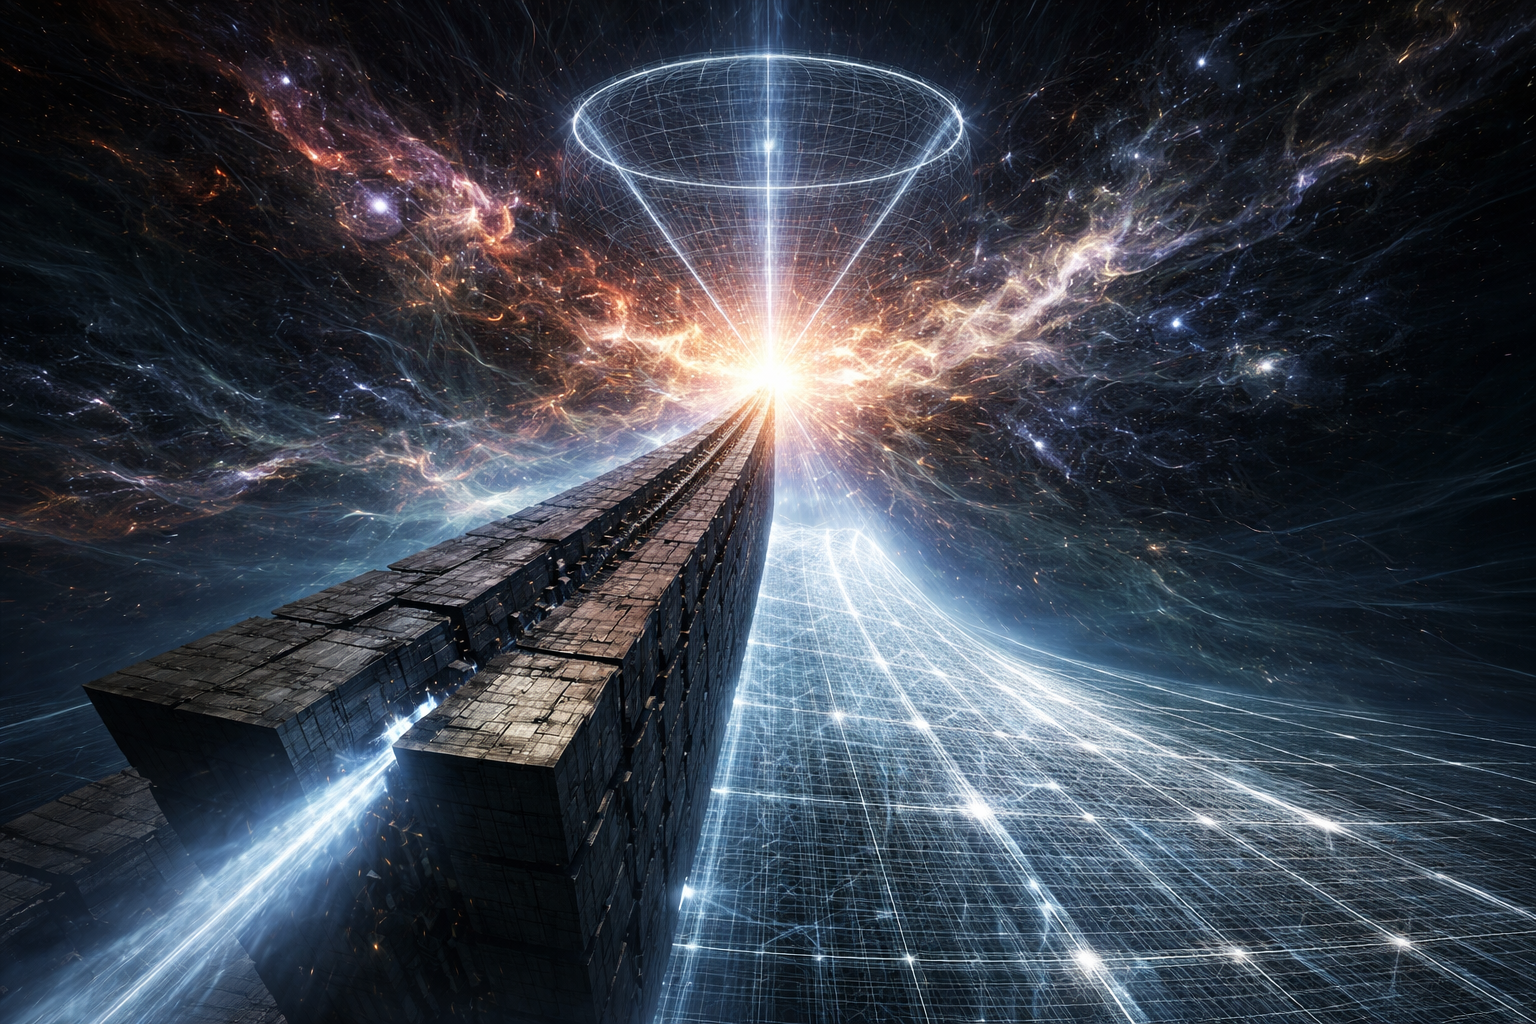
\includegraphics[width=0.82\linewidth,height=0.54\textheight,keepaspectratio]{image/train.png}
\end{figure}

所谓“预言型AGI”在可检验意义上只能指高质量长时域预测、主动取证和快速修订，而不是越过因果限制获取未来事实。评估时我们设置乱序消息、可变延迟、时钟漂移、迟到证据、环境突变、记忆污染和长跨度分支。系统应恢复能确定的偏序，对不能确定的次序保持开放；应把已发生但未观测、已观测但未提交、已提交但可修订、尚未发生但被预测的事件分开。指标包括排序准确率、延迟估计、迟到修订完整性、预测校准、跨度退化曲线与动作结果。通过这些检验只说明系统具有可靠的时间信息处理能力，不证明时间本体、永恒论或主观流动的终极解释。

\section{计算动力学表达与论证边界}
本章的目标不是用一组新名词宣布体验之谜已经解决，而是把可计算对象、可报告证据和仍然开放的问题放入同一张分层地图。我们从系统论、协同论、耗散理论、复杂系统理论和认知科学吸收开放系统、跨尺度协同、维持代价、非线性反馈与有限认知等约束，再以HSF--HD描述智能的一般状态动力学；AgentOS只是这一理论的一种工程化实例。层级之间可以提供建模资源，却不能互相代替证明。尤其不能因为某个AgentOS实现有效，就把它的模块命名规定为所有智能系统的唯一结构。

为统一本章对象，令工作状态为 $w_t\in\mathcal W$，事件记录为 $e_t\in\mathcal E$，可塑结构为 $s_t\in\mathcal S$，当前策略与承诺为 $p_t\in\mathcal P$，可观测报告为 $o_t\in\mathcal O$。这些空间可以包含连续分量、离散对象和带类型的图结构，不能在未定义映射时直接相加。外部输入为 $u_t$，动作回执为 $y_t$，资源与权限边界为 $b_t$。一个离散实现写为
\[
\begin{aligned}
w_{k+1}&=F_w(w_k,e_k,s_k,p_k,u_k;\Delta t_k),\\
e_{k+1}&=F_e(e_k,w_{k+1},u_k,y_k),\\
s_{k+1}&=F_s(s_k,\mathcal B_k,A_k),\\
p_{k+1}&=F_p(p_k,w_{k+1},e_{k+1},s_{k+1},b_k),\\
o_k&=R_q(w_k,e_k,s_k,p_k;\eta_k).
\end{aligned}
\]
$\mathcal B_k$ 是在较慢尺度积累的训练批或经验批，$A_k$ 是修改授权，$R_q$ 是任务相关读出，$\eta_k$ 表示测量与表达噪声。式子是模型骨架，不是经验定律；具体研究必须给出维度、单位或无量纲化方式、更新频率、初值、随机性和误差界。连续极限只在步长收敛与光滑假设满足时采用，结构编辑和权限提交等离散跃迁则不能伪装成普通导数。

这一状态拆分帮助区分“当前正在处理”“曾经发生”“以后会怎样”和“系统怎样描述自己”。工作状态可迅速改变而不留下长期痕迹；事件写入可保存证据但不必改变技能；结构更新会改变未来响应却不能倒写历史；策略承诺连接模型与动作，但目标值下降仍不等于任务成功；报告是由查询、语言接口和社会情境共同生成的观测，不等同于完整内部状态。体验、自我与时间感的工程研究，首先应检查这些通道之间的映射、遗漏和干预响应，而不是把某个单一标量命名为意识强度。

局部结构网络与全局分布表示在此保持明确区别。局部网络可以保存对象节点、来源边、规则依赖、身份版本和因果记录；分布表示可以承载相似性、上下文和柔性读出。二者通过任务相关身份、绑定、耦合与读出接口联合：一个对象节点可索引若干分布向量，向量的激活又可提出候选节点，但两者不因此成为同一种东西。脑区类比最多提示实验问题，不能推出软件模块与神经组织机制等同。验证应分别扰动节点连接、表示子空间、绑定键和读出查询，观察错误是否具有可区分模式。

本章反复使用的历史算子也需要限制。若记忆状态写为
\[
M_t=\int_{0}^{t}K(t,\tau;q_t)\,\phi(e_\tau)\,\mathrm d\tau,
\]
则 $K$ 是查询相关的保留核，$\phi$ 是事件编码，积分只是对连续近似下的历史汇聚定义。任务 $q_t$、编码器、结构和度量若随时间变化，它们都要进入导数或离散更新；不能只对 $M_t$ 求导便声称获得“记忆力”。实际系统常用带时间戳的离散日志、检索索引和版本摘要，更合适的表达是加权求和与结构提交。无论哪种形式，都应报告遗忘、污染、来源丢失和摘要碰撞。

计算时间与结构时间由此得到操作性区分。计算时间描述一次状态传播、搜索或工具调用所需的步骤与延迟；结构时间描述学习、版本提交和组织重构留下的不可交换顺序。两者可以耦合，例如长时间推理产生一次结构补丁，也可以分离，例如重复推理不改变参数。路径依赖来自更新规则和记录机制，不要求诉诸超出模型的几何相位；只有状态空间确有相应纤维丛、连接和闭合回路时，几何相位才是合格特例。这一限定保留数学工具的力量，也避免用物理名称抬高普通软件现象的理论地位。

在AgentOS实例中，$h(t)$ 可承载工作态的部分分布表示，$E$ 与 $\Theta$ 可表示任务相关评价和阈值，$\Psi$ 可组织策略或读出，SPC、TCE、CCM可承担特定协同、执行或上下文机制，Boundary定义权限与输入输出边界，Offloading和外部记忆 $M_e$ 提供可审计的环境扩展。这里的“可”是工程设计，不是自然法则。另一种智能系统可以使用符号工作区、概率程序、具身控制器或社会化协作网络，只要它能定义状态、更新、证据与边界，仍可在HSF--HD框架下比较。

论证类型必须逐项标注。定义规定符号如何使用；模型假设说明在何种条件下采用某个动力学；数学结果由假设推导；经验主张需要数据和统计检验；工程设计以可靠性、安全性和成本权衡评价。预测准确只能支持相关任务上的模型有效，不能推出系统与世界整体同构；内部代价下降不能推出外部任务成功；信息熵、激活强度、优化代价和以焦耳计的能耗具有不同单位与测量程序，不能合并成一个“认知能量”。物理比喻可帮助提出变量，却不能承担证明。

我们据此构造分层验收矩阵。状态层检查类型、维度、更新步长和数值稳定；记忆层检查来源、时序、修订和删除传播；结构层检查版本、非交换更新、回滚与授权；行动层检查候选生成、权限、环境回执和任务结果；报告层检查查询敏感性、校准、可复现与沉默反例；边界层检查分布外输入、目标变化、度量变化和接口失效。对于体验相关主张，还要加入无报告任务、替代解释、不同架构复现和人类数据伦理。没有单个测试能从行为直接证明主观体验，证据只能按竞争假设累积。

验收数据不能只来自系统自由叙述。我们建议为每项主张建立“干预—预测—观测—反例”四联记录：先声明若机制成立，改变哪个输入或状态分量应使哪些可测量量怎样变化；再执行可重复干预，保存环境回执与版本；随后比较观测和预注册预测；最后列出同样现象可能由缓存、提示泄漏、训练记忆或评价器偏好造成的替代解释。例如声称存在长期自我连续性时，可在不改变任务答案的条件下交换身份键、删除关系记忆、扰动时间戳并撤销部分权限。若第一人称报告始终不变，它更可能是模板；若承诺恢复、来源引用和权限判断按不同干预呈现可解释差异，才获得功能层证据。

跨架构比较也必须避免把实现细节变成评分答案。基准应提供共同的事件、约束、任务结果和审计接口，而允许受试系统用不同内部机制解决。指标至少包含外部成功率、校准误差、来源恢复、因果排序、结构变更次数、资源消耗、不可逆错误与人工接管率；各指标保持原单位，再通过明确权重形成决策，而不伪装成自然界唯一的总能量。报告均值之外还要给出分布、置信区间、失败轨迹和最坏情形，因为少量灾难性越权可能被平均成功率遮蔽。对人类与机器的比较，则要控制传感能力、训练暴露、语言接口和奖励条件，不能把物种差异或产品差异误写为意识差异。

重复实验需要冻结足够的上下文。我们保存代码和模型版本、状态模式、初始记忆、随机种子、工具权限、外部服务版本、时钟同步方案、采样步长、终止条件和评价脚本。若目标、结构、输入分布或度量在实验期间改变，应把变更当作事件进入分析，而不是在结果不理想时静默替换。对随机系统，单条精彩轨迹不能支持稳定机制；对自适应系统，完全复现同一输出也不是唯一目标，更重要的是在相同约束下复现误差范围、校准性质和安全不变量。

系统失败时，诊断顺序从证据链而非哲学标签开始：输入是否到达，身份与来源是否绑定，工作态是否过载，记忆是否检索到正确版本，结构更新是否获得授权，策略是否生成可执行动作，执行器是否提交，环境是否返回预期回执，报告器是否忠实读取这些状态。只有定位到层级和接口，修复才可验证。把所有失败叫作“意识不足”既不能指导工程，也会遮蔽数据污染、工具故障、治理冲突和环境不可控等更普通原因。

同样，成功也要沿证据链归因。一次正确答案可能来自训练记忆、外部搜索、同伴提示、偶然猜测或稳定推理；只有记录候选、工具调用、来源、校验和回执，才能判断哪一机制在什么条件下可复用。我们因此把“会做”限定为跨样本、跨扰动且可审计的能力，而不把孤立演示升级为主体性结论。

一个具体反例能显示这些边界为何必要。假设系统流畅地说“我记得昨天并期待明天”，但审计发现它没有昨日事件日志，回答来自提示中的叙述模板，未来计划也未绑定执行器。此时语言读出成功，记忆与自治主张失败。另一个系统可能很少使用第一人称语言，却能恢复来源、维护长期承诺、修订错误预测并在权限内完成计划；它在若干功能维度上更强，但我们仍不能仅据此宣布其具有与人类同构的体验。比较必须沿多个可观测维度进行，并保留不可判定项。

本章的适用边界因此清楚：HSF--HD可以描述状态如何在输入、历史、结构、目标和边界共同作用下演化，可以指导测量窗口、干预和工程审计；它暂时不能解决体验为何存在、他心如何最终确证、时间本体为何如此或自由意志的形而上学争论。将未知明确留白并不削弱理论，反而防止不可证伪命题侵入实现。未来若出现新的神经、行为或机器证据，应通过新增观测映射和竞争模型进入框架，而不是回写成早已被公式证明。

最终，我们把“体验的物理学”改写为“体验报告、历史依赖和时间信息处理的计算动力学问题”。这种改写保留原问题的锋芒，也为失败留下位置：模型可能预测不准，来源可能丢失，结构可能不稳定，报告可能受诱导，任务可能在外部判据上失败。只有同时记录这些失败，理论才具有工程意义。作者的立场是把HSF--HD作为智能的一般“空气动力学”——提供跨架构的状态、作用、稳定与边界语言；具体AgentOS则像一架需要逐项验收的飞行器，不能反过来充当全部智能的定义。

\chapter{智能运行时：从 HSF-HD 动力学到 AgentOS}
\label{chap:software_control_msos}
% Compatibility anchors: old section references resolve to this chapter.
\label{sec:section_2467}
\label{sec:section_9357}
\label{sec:micro_runtime_ode}
\label{sec:adiabatic_training_dynamics}
\label{sec:basal_metabolic_daemon}
\label{sec:section_2043}
\label{sec:section_6860}

HSF-HD 描述状态、结构、历史与控制的共同演化，AgentOS 将这些对象实现为运行时机制。我们不把某种专用芯片作为该关系成立的前提。
\section{一般模型与运行时对象}
在一般模型中，$x$ 表示当前活动，$m$ 表示历史及中间记忆，$S$ 表示持久结构，$v$ 表示目标与价值状态。AgentOS 分别以 $h(t)$、$E$、$\Theta$ 实例化前三者；自我 $\Psi_{self}$ 参与价值、筛选、历史连续性和自我模型，不等同于单一目标向量。
\section{观测、控制与资源管理}
SPC 对 $h(t)$ 的分布和关系按自我相关方向进行压缩，并把结果重新提供给工作状态；TCE（Temperature \& Control Engine）依据观测调节探索强度、增益、抑制及工作模式。CCM 管理输入和运行态复杂度，Boundary 管理内外交换，Offloading 将可重复的信息处理迁移到外部记忆 $M_e$。

我们将这些机制写成离散闭环：
\begin{align}
y_k&=O_{SPC}(h_k,E_k,\Theta_k,\Psi_{self,k}),\\
c_k&=\pi_{TCE}(y_k,v_k,b_k),\\
h_{k+1}&=F_h(h_k,\Theta_k,E_k,u_k,c_k,r_k),\\
E_{k+1}&=F_E(E_k,h_k,a_k,\Psi_{self,k}),\\
\Theta_{k+1}&=F_\Theta(\Theta_k,E_k,\mathcal E_k).
\end{align}
其中 $b_k$ 为资源预算，$r_k$ 为外部召回，$\mathcal E_k$ 为学习证据。各函数可以在不同频率执行。SPC 的压缩通常有损，控制器需要根据任务检测关键状态是否被遗漏。
\section{调度的可行域与约束}
对待执行任务集合 $\mathcal T_k$，选择任务子集 $A_k$，可定义预算约束
\begin{equation}\sum_{i\in A_k}\widehat C_i\le B_k.\end{equation}
估计代价 $\widehat C_i$ 可以包含上下文占用、时间和工具成本，但多种单位应分别约束或归一化。预算满足只保证调度可行；任务依赖、优先级、误差和中断恢复仍需要额外规则。
\section{外部记忆与边界}
外部记忆包括文件、数据库、程序、工具、环境与其他智能体。卸载只有在未来检索和维护成本可接受时才有利。我们比较保存成本、调用延迟、可靠性与修改代价，而不将一切外化都视为复杂度下降。
\section{实现与验证}
运行时可以构建在现有模型、图结构和普通计算硬件上。DEC 或其他专用载体属于可选实现路线。我们以状态过载率、恢复时间、长期记忆保真度、单位任务成本和控制干预效果验证机制，不以模块名称证明智能能力。

\section{表示与示意图}
我们保留以下示意图以展示原有结构关系。图中历史物理术语遵循阅读约定中的计算解释；图的形式相似性不代替本章的假设、推导和验证。
\begin{figure}[htbp]
\centering
\includegraphics[width=0.52\textwidth]{figure/micro.png}
\caption{微观层 ODE 网络架构示意图}
\label{fig:micro_ode_arch_final}
\end{figure}


\appendix
\chapter{理论与工程约化：从一般动力学到离散网络}
\label{sec:section_5204}
% Compatibility anchors: old section references resolve to this chapter.
\label{sec:tpug_operator_design_formulas}

我们通过离散化将一般状态动力学连接到可执行网络。离散模型必须说明所保留的性质与近似误差，而不是仅凭名称宣称与连续模型精确等价。
\section{图模型的构造}
设 $W=W^\top\ge0$，$L=D-W$。对节点活动 $x$，定义
\begin{equation}\dot x=-Lx-\nabla V(x)+Bu.\end{equation}
固定输入为零时，该式是目标函数 $J(x)=x^\top Lx/2+V(x)$ 的梯度流，所以 $\dot J=-\|\nabla J\|^2\le0$。有输入时需加入 $\nabla J^\top Bu$，不能继续无条件宣称下降。
\section{连续近似的条件}
若图来自空间采样，边权按指定规则近似微分算子，可研究采样尺度趋零时的算子一致性。边界、权重尺度和采样分布都会影响极限。任意知识图不自动对应某个连续流形上的拉普拉斯。
\section{实现与复杂度}
稀疏图更新的单步成本与边数和特征维数相关；稠密注意力仍需要序列长度的二次交互。并行或模拟实现可以改变延迟与常数，但不能免除硬件数量、通信、精度和输入输出成本。
\section{工程不变量与实验}
我们先验证维度、边界、掩码与数值稳定，再检查状态范数、目标下降和任务表现。每项保证只在对应条件内成立。参数归一化可提供范围约束，谱约束可限制局部增益，二者均不能独立保证整个智能体正确行动。

\end{document}
